\documentclass[8pt]{extarticle}
\usepackage{makeidx}
\usepackage{tocloft}
\usepackage{setspace}
\renewcommand{\contentsname}{Indice dei contenuti}
\renewcommand{\cftsecleader}{\cftdotfill{\cftdotsep}}
\usepackage{graphicx}
\usepackage{amsmath}
\usepackage{amssymb}
\usepackage{latexsym}
\usepackage{subcaption}
\renewcommand\refname{Referenze}
\usepackage[utf8x]{inputenc}
\usepackage{titlesec}
\usepackage{bm}
\usepackage{mathtools}
\usepackage[document]{ragged2e}
\titleformat{\section}{\huge\normalfont\bf}{\thesection.\hspace{5pt}}{5pt}{\vspace{1cm}}
\titleformat*{\subsection}{\Large\bfseries}
\usepackage[inner=3cm,outer=3cm]{geometry}

\makeindex

\begin{document}
\Large{A.a. 2014-2015}
\vspace{10cm}
\begin{center}
\Huge\textbf{Simulazione di uno spettrometro per il decadimento $K^0_S \rightarrow \pi^+ \pi^-$}
\end{center}

\vspace{2cm}
\begin{flushleft}
\medskip
\textit{Studente:} 
\hspace{10 cm}
\textit{Docente:} \\
\medskip
Federico \textsc{Massa}
\hspace{9 cm}
Sergio \textsc{Giudici}
\end{flushleft}



\newpage

\begin{abstract}	
\justify
Il progetto realizzato consiste nella simulazione di uno spettrometro per la ricostruzione dell'impulso di un fascio puro di $K^0$ di impulso distribuito gaussianamente $100 \pm 5\ GeV/c$ utilizzando il decadimento $K^0_S \rightarrow \pi^+ \pi^-$. Con un apparato sperimentale di $73\ m$ di lunghezza, circa $0.5\ m$ trasversali e uno spettrometro con $p_{kick} = 0.105\ MeV/c$ è stata confrontata la risoluzione ottenuta con un fit cinematico con vari vincoli.  La ricostruzione migliore utilizzata ha portato ad una risoluzione sull'impulso del $K^0$ di $1.0\ GeV/c$.
\end{abstract}
\bigskip

\doublespacing
\tableofcontents
\singlespacing

\newpage

\section{Introduzione} \label{sec:intro}
\justify
Il presente progetto consiste nella simulazione di uno spettrometro per la ricostruzione dell'impulso di un fascio puro di $K^0$ di impulso $100 \pm 5 \ GeV/c$, distribuito gaussianamente.
\medskip

Scopo del progetto è quello di misurare la risoluzione del suddetto spettrometro al variare della tecnica di ricostruzione utilizzata e del numero di rivelatori utilizzati nell'apparato sperimentale. Ai fini della simulazione è stato considerato solamente il decadimento del $K^0_S \rightarrow \pi^+ \pi^-$. 

Il codice utilizzato è stato scritto interamente in C++, con l'ausilio delle librerie ROOT del CERN per la visualizzazione e il salvataggio in memoria dei dati. \\

\section{Apparato sperimentale simulato} \label{sec:apparato}
L'apparato simulato appare come in Fig. \ref{fig:apparato_3d}, \ref{fig:apparato_2d}.


\begin{figure}
	\begin{center}
		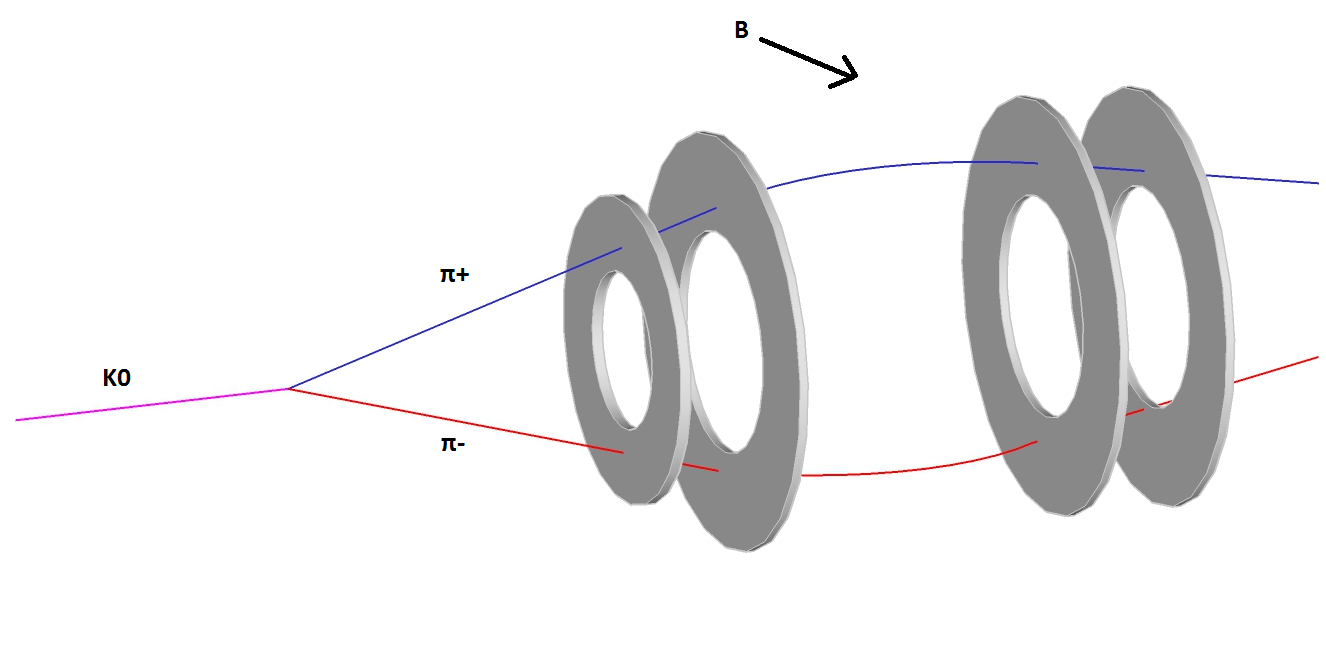
\includegraphics[scale=0.4]{apparato_3d} 
		\caption{Riproduzione 3D dell'apparato sperimentale: con $\vec{B}$ è indicato il vettore del campo magnetico, nella direzione positiva delle $x$.}
		\label{fig:apparato_3d}
	\end{center}
\end{figure}

\begin{figure}
	\begin{center}
		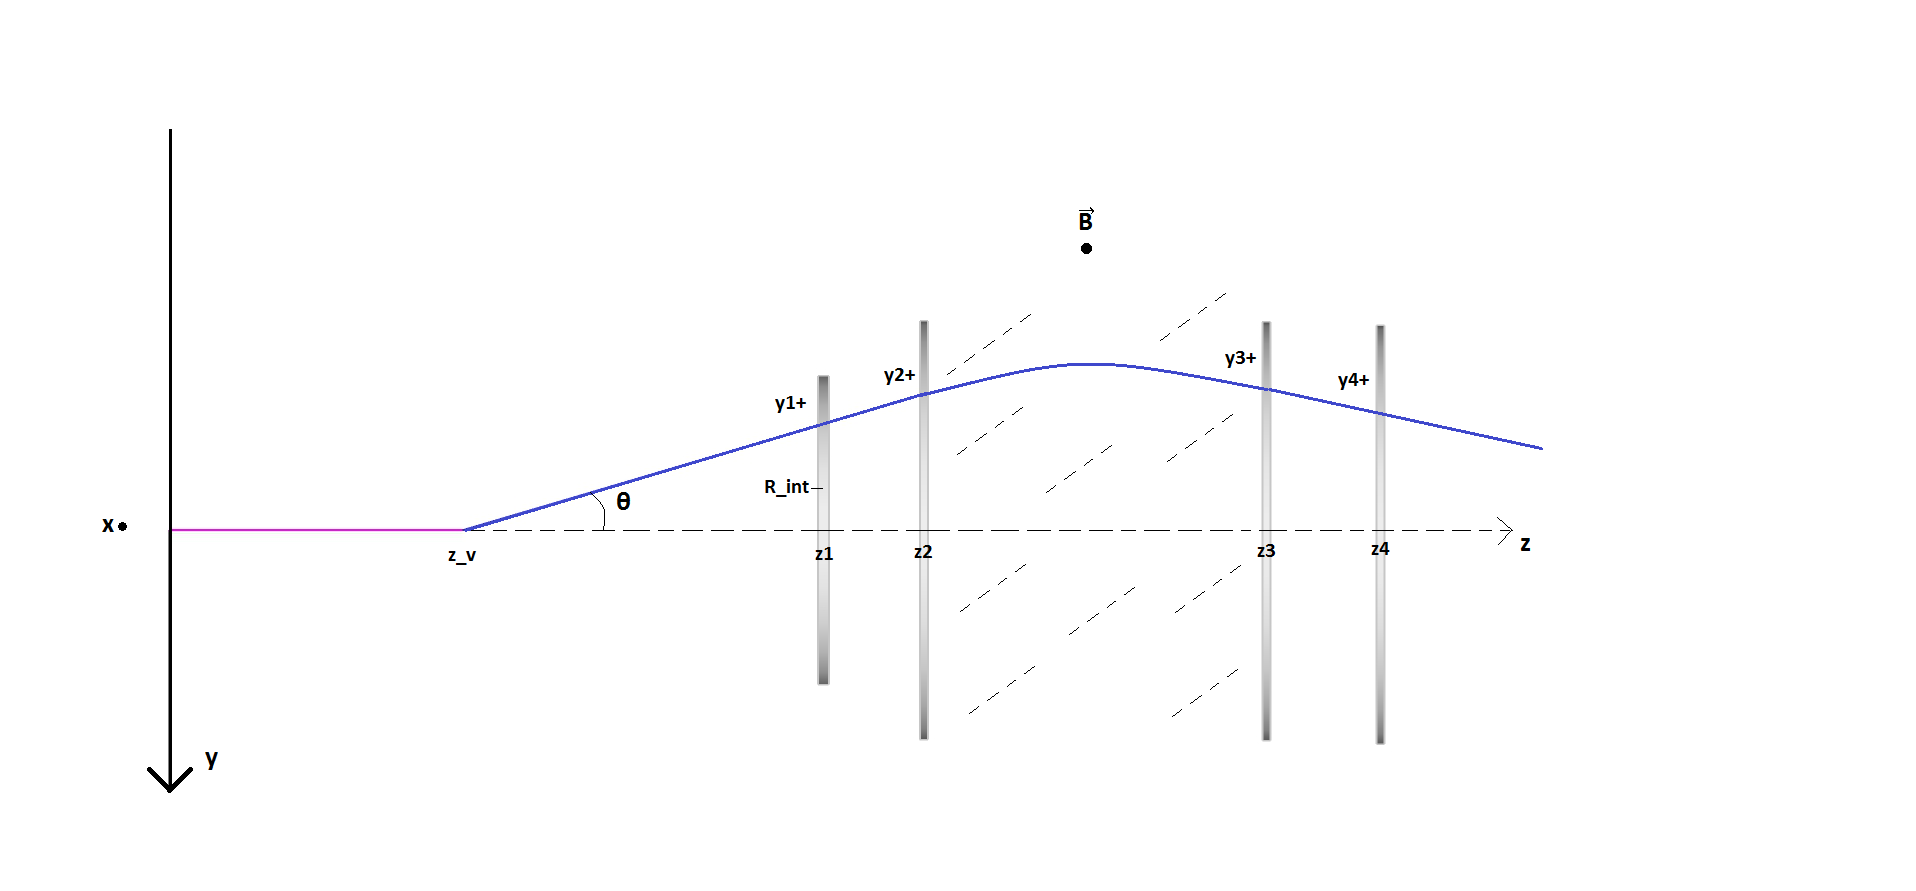
\includegraphics[scale=0.4]{apparato_2d}
		\caption{Sezione dell'apparato sperimentale: in viola lungo l'asse z, la traccia del $K^0$ genitore, in blu una possibile traccia di un $\pi^+$. Il campo magnetico, nella direzione positiva delle $x$, è uscente perpendicolarmente dal piano della figura. Con $z_i$ sono indicate le coordinate $z$ dei quattro piani di rivelatore. Con $R_{int}$, invece, il raggio interno del rivelatore più vicino. Con $y_i^{\pm}$ invece si intende la coordinata y del piano i-esimo corrispondente alla traccia di un $\pi^{\pm}$.}
		\label{fig:apparato_2d}
	\end{center}
\end{figure}

Ogni piano di rivelatore è modellizzato da una corona circolare di raggio interno $R_{int}$ e raggio esterno $R_{ext}$, con risoluzione fissa sugli assi $x$ e $y$ di $1\ mm$\footnote{Come si vedrà in Sez.\ref{sec:detector}, la risposta del rivelatore è assunta gaussiana e la risoluzione indicata è dunque uguale alla deviazione standard di questa distribuzione.}. Sebbene il raggio esterno sia importante a livello pratico nel disegno del rivelatore, ai fini di questa simulazione questo sarà sempre considerabile infinito, poiché scelto in modo tale da contenere l'interezza dei decadimenti. La scelta del raggio interno è invece soggetta a differenti necessità, che saranno discusse più avanti (Sez. \ref{subsec:raggio_interno}). Il campo magnetico è situato in una zona di $\Delta L = 0.35\ m$ al centro tra i piani $2$ e $3$, che distano tra loro $3\ m$ e vale $B = 1\ T$. Il $p_{kick}$ corrispondente vale quindi circa $p_k = qB\Delta L = 105\ MeV/c$. La modellizzazione dell'effetto di un magnete come un kick effettuato nel punto medio tra i rivelatori sarà giustificata in sez.\ref{sec:generation}. In Tab.\ref{tab:apparato} sono riassunte le caratteristiche scelte per l'apparato e la lunghezza media di decadimento, ovvero $\mathbf{<\lambda>} = \frac{<p>}{M_{K}} c \tau$, $\tau = 8.954 \cdot 10^{-11} \ s$. 

\bigskip

\begin{table} [h!]
\centering
\begin{tabular}{||p {1.5 cm}|p {1 cm}||}
\hline \hline
$\mathbf{{<\lambda>}(m)}$ & 5.4 \\ 
\hline
$\mathbf{z_1(m)}$ & 50 \\ 
\hline
$\mathbf{z_2(m)}$ & 60 \\ 
\hline
$\mathbf{z_3(m)}$ & 63 \\ 
\hline
$\mathbf{z_4(m)}$ & 73 \\
\hline
$\mathbf{R_{int, 1}(m)}$ & 0.08 \\
\hline
$\mathbf{R_{ext, 1}(m)}$ & 0.46 \\
\hline
$\mathbf{R_{int, 2}(m)}$ & 0.09 \\
\hline
$\mathbf{R_{ext, 2}(m)}$ & 0.56 \\
\hline
$\mathbf{R_{int, 3}(m)}$ & 0.10 \\
\hline
$\mathbf{R_{ext, 3}(m)}$ & 0.60 \\
\hline
$\mathbf{R_{int, 4}(m)}$ & 0.10 \\
\hline
$\mathbf{R_{ext, 4}(m)}$ & 0.70 \\
\hline
$\mathbf{p_k}(MeV/c)$ & 105 \\
\hline
$\mathbf{B}(T)$ & 1 \\
\hline
$\mathbf{\Delta L}(m)$ & 0.35 \\
\hline
$\mathbf{\sigma_x}(m)$ & 0.001 \\
\hline \hline
\end{tabular} 
\caption{Tabella riassuntiva delle caratteristiche dell'apparato sperimentale.}
\label{tab:apparato}
\end{table}

\section{Struttura del codice} \label{sec:script}
Il codice, scritto in C++, presenta una struttura modulare rappresentata in un diagramma in Fig.\ref{fig:script_structure}.

\begin{figure}
	\begin{center}
		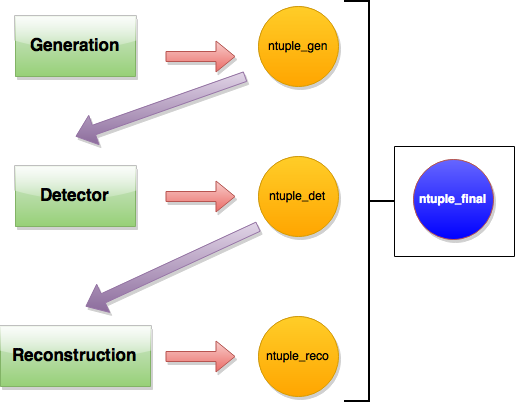
\includegraphics[scale=0.4]{script_structure}
		\caption{Diagramma di flusso del funzionamento del codice. Ogni modulo riceve in input e/o produce in output una \textit{ntupla}.}
		\label{fig:script_structure}
	\end{center}
\end{figure}

Esso si basa sull'uso di una classe di ROOT, \textit{TNtupleD}, alle cui istanze ci riferiremo con il nome \textit{ntuple}, che permette di salvare in un file tutte le caratteristiche desiderate per un evento in forma di variabili in doppia precisione. \\

Il codice consiste di tre moduli: \\
\begin{itemize}
\item \textit{Generation}: grazie all'uso di un generatore di numeri pseudocasuali (\textit{TRandom3}), si serve di una classe chiamata \textit{KGen} per generare le caratteristiche di un singolo evento. Iterando questo procedimento, vengono generati tutti gli eventi e salvati in una ntupla chiamata \textit{ntuple\_gen}.
\item \textit{Detector}: utilizzando come input \textit{ntuple\_gen}, si occupa di trovare i punti di passaggio dei prodotti di decadimento nei rivelatori e di effettuare uno \textit{smeering} gaussiano per simulare la risposta del rivelatore. Si serve della classe \textit{B\_event} per simulare l'effetto del campo magnetico. Gli hit trovati vengono salvati nella ntupla \textit{ntuple\_det}.
\item \textit{Reconstruction}: utilizzando come input \textit{ntuple\_det}, che contiene solo le informazioni fruibili allo sperimentatore, si occupa di effettuare un fit cinematico con vincoli e parametri non misurati per trovare delle misure migliorate, che vengono scritte in \textit{ntuple\_reco}.
\end{itemize}

Le informazioni provenienti dalle tre ntuple vengono infine unite in una sola, chiamata \textit{ntuple\_final}, che permette di studiare la risoluzione dello spettrometro confrontando la misura migliorata dell'impulso con quella generata. Nelle prossime sezioni analizzeremo nel dettaglio i tre moduli. \\

\section{Generazione dell'evento} \label{sec:generation}

Il modulo \textit{Generation} si basa sulla classe \textit{KGen}, che genera i singoli eventi tramite il metodo \textit{Generate} e su un main, che richiama un numero predeterminato di volte questo metodo e ne salva i risultati volta per volta su \textit{ntuple\_gen}. Il main ha anche a disposizione l'opzione per generare eventi con punto di decadimento costante. \medskip
Da questo momento le variabili contrassegnate da $*$ si intendono nel sistema del centro di massa, mentre quelle senza in quello del laboratorio.
Nel decadimento preso in esame la particella madre, il $K^0$, è scalare, per cui non vi può essere alcuna direzione privilegiata nel decadimento nel sistema del centro di massa. Questo comporta che i prodotti di decadimento presentino una distribuzione angolare piatta in $\mathit{\cos{\theta^*}}$ e $\mathit{\phi^*}$, dove il sistema di coordinate scelto è quello polare con polo nel punto di decadimento. $\theta^*$ è dunque calcolato come $cos^{-1}(\cos{\theta^*})_{gen}$ ed è dunque compreso tra $0$ e $\pi$, mentre $\phi$ è generato uniformemente tra $0$ e $2\pi$. Una volta generata la direzione del primo prodotto, il secondo è automaticamente determinato dalla legge di conservazione dell'impulso. Risulta: \\
$$
\theta_2^* = \pi - \theta_1^*
$$
$$
\phi_2^* = \phi_1^* + \pi
$$

dove a $\phi_2^*$ si sottrae $2\pi$ se $\phi_2^* > 2\pi$. 


Essendo un decadimento a due corpi identici in massa, inoltre, l'energia dei prodotti ha un valore ben preciso ed uguale per i due prodotti, così come quello degli impulsi: 
$$
E_1^* = E_2^* = \frac{M_K}{2}
$$
$$
p_i^* = \sqrt{E_i^{2*} - M_\pi^2}
$$

Si procede dunque a generare l'impulso del K secondo una distribuzione gaussiana con media $100\ GeV/c$ e deviazione standard $5\ GeV/c$, e si calcola la sua $\beta$ come
$$
\beta = p_K/E_K \approx 1 - \frac{1}{2} \frac{M_K^2}{p_K^2}
$$

Con questo valore si possono trovare gli impulsi nel sistema del laboratorio con un boost lungo z con $\beta_{boost} = -\beta$. 
Per quanto riguarda gli angoli, sono calcolati tramite: 

$$
\cos{\theta_i} = \frac{p_{zi}}{p_i}
$$
$$
\phi_i = atan2(p_{ix}, p_{iy}) = \phi_i^*
$$

Per quanto riguarda la z di decadimento, viene generata con distribuzione esponenziale e lunghezza di decadimento dipendente dall'energia del $K^0$ generato:
$$
z_v \sim Exp(z_v | \lambda = \beta\gamma c \tau)
$$

Queste funzionalità sono accessibili dal main tramite i metodi pubblici \textit{GetTheta}, \textit{GetP}, ... della classe \textit{KGen}.

In Fig. \ref{fig:gen_pK}, \ref{fig:gen_z}, \ref{fig:gen_theta}, \ref{fig:gen_phi}, \ref{fig:gen_p}, \ref{fig:gen_thetatheta}, \ref{fig:gen_thetap}, \ref{fig:gen_mintheta} sono rappresentate alcune distribuzioni degli eventi generati.

\begin{figure}
	\begin{center}
		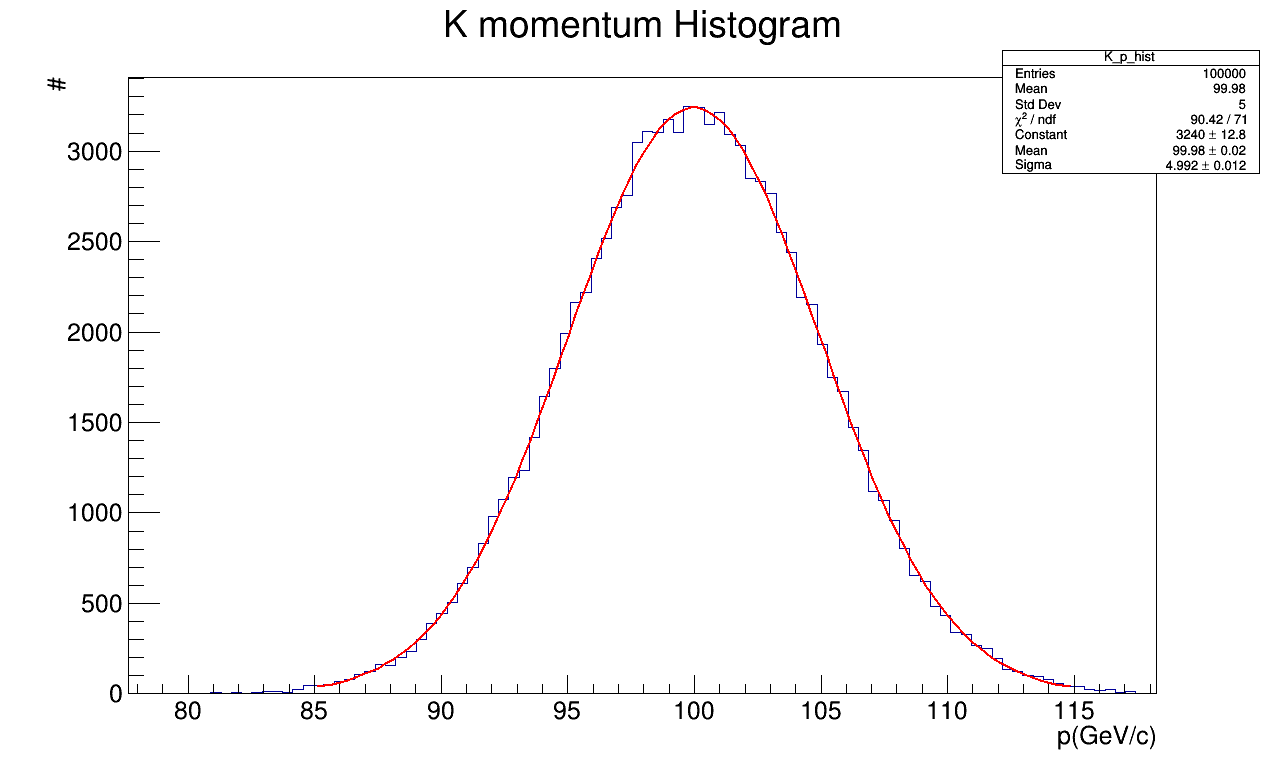
\includegraphics[scale=0.3]{gen_pK} 
		\caption{Distribuzione dell'impulso generato del $K^0$ e fit gaussiano.}
		\label{fig:gen_pK}
	\end{center}
\end{figure}

\begin{figure}
	\begin{center}
		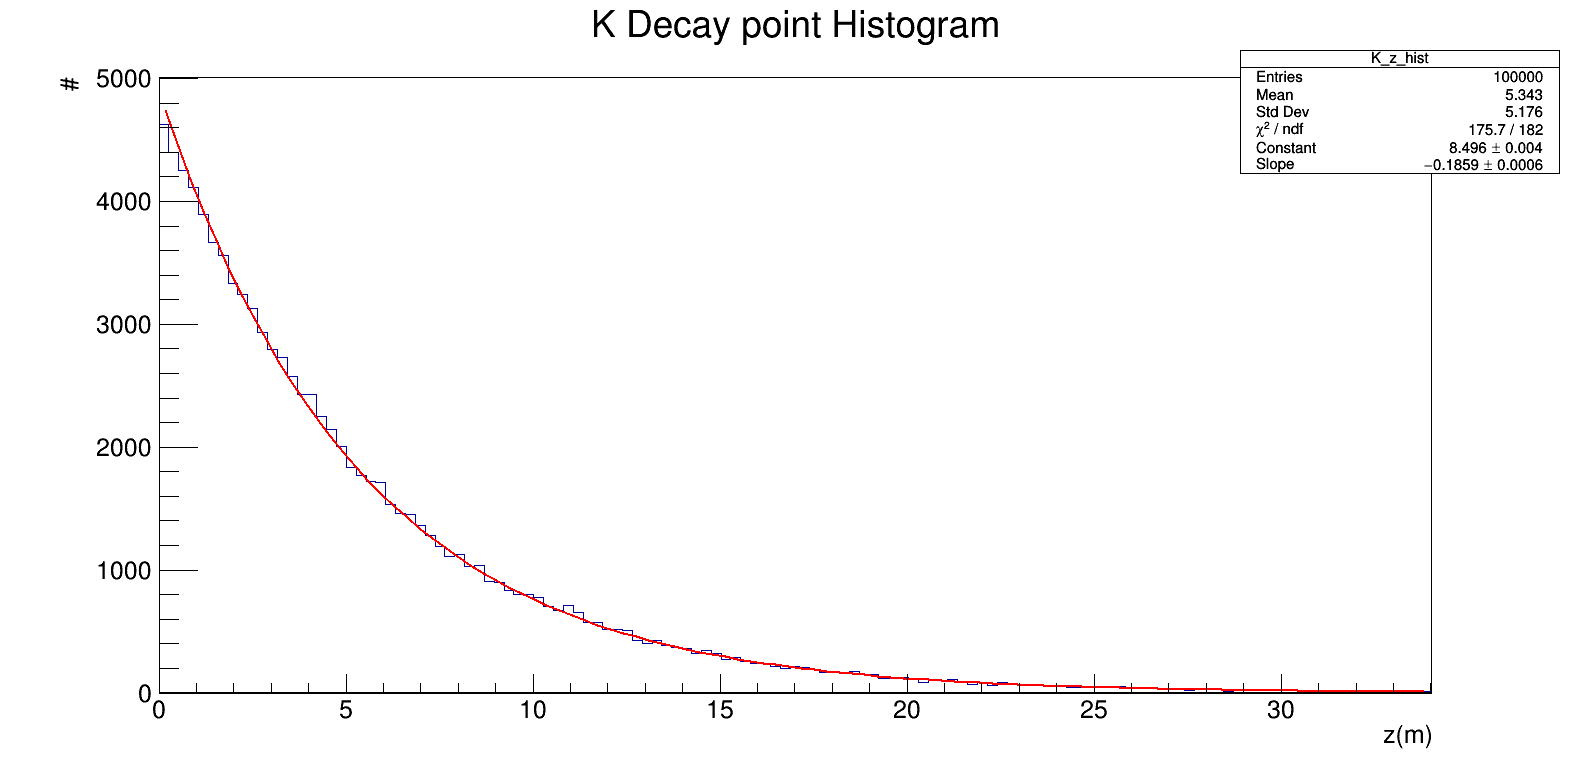
\includegraphics[scale=0.3]{gen_z} 
		\caption{Distribuzione della z di decadimento e fit esponenziale. In realtà la distribuzione vera si discosta da un'esponenziale a causa della distribuzione dell'impulso del $K^0$.}
		\label{fig:gen_z}
	\end{center}
\end{figure}

\begin{figure}
	\begin{center}
		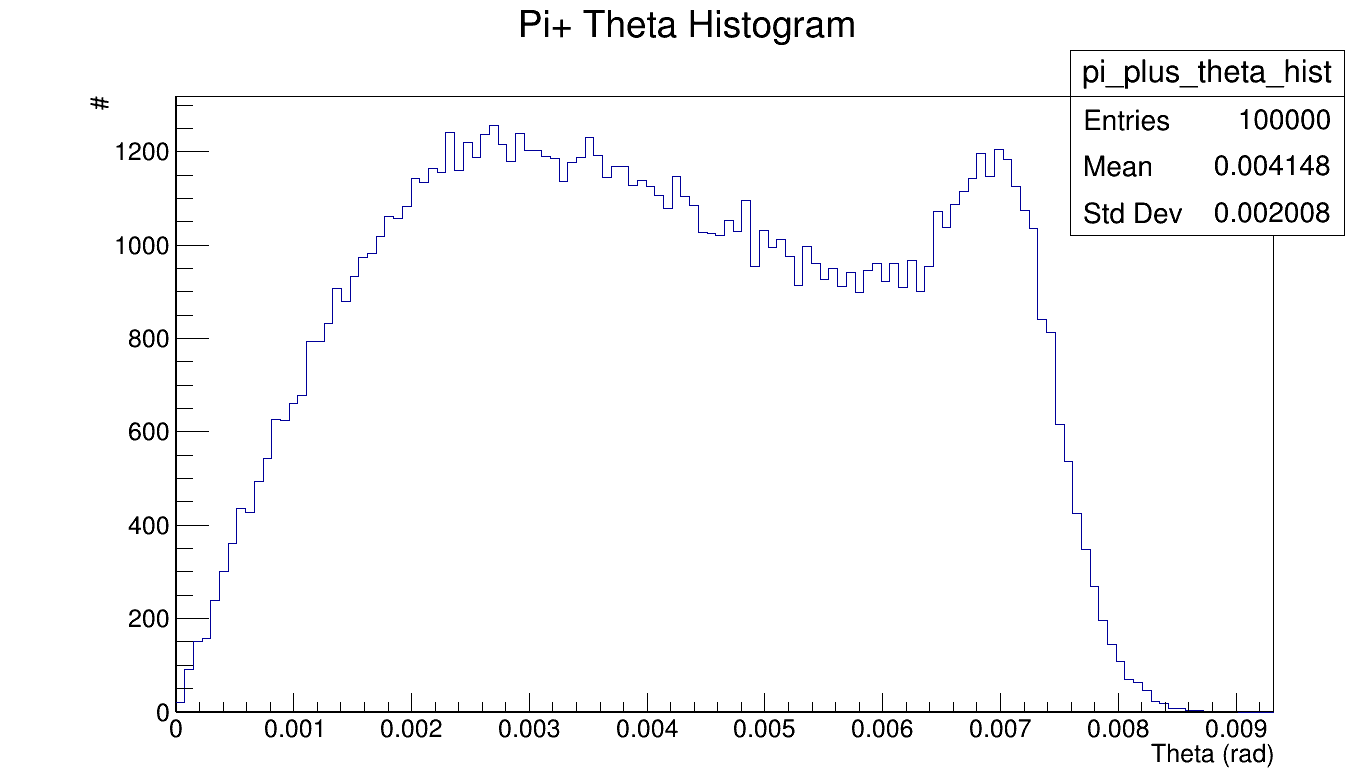
\includegraphics[scale=0.3]{gen_theta} 
		\caption{Distribuzione dell'angolo $\theta$ nel caso del $\pi^+$. La distribuzione è limitata superiormente ad un valore inferiore a $\pi$ a causa del boost. Nel caso del $\pi^-$ la distribuzione è analoga.}
		\label{fig:gen_theta}
	\end{center}
\end{figure}

\begin{figure}
	\begin{center}
		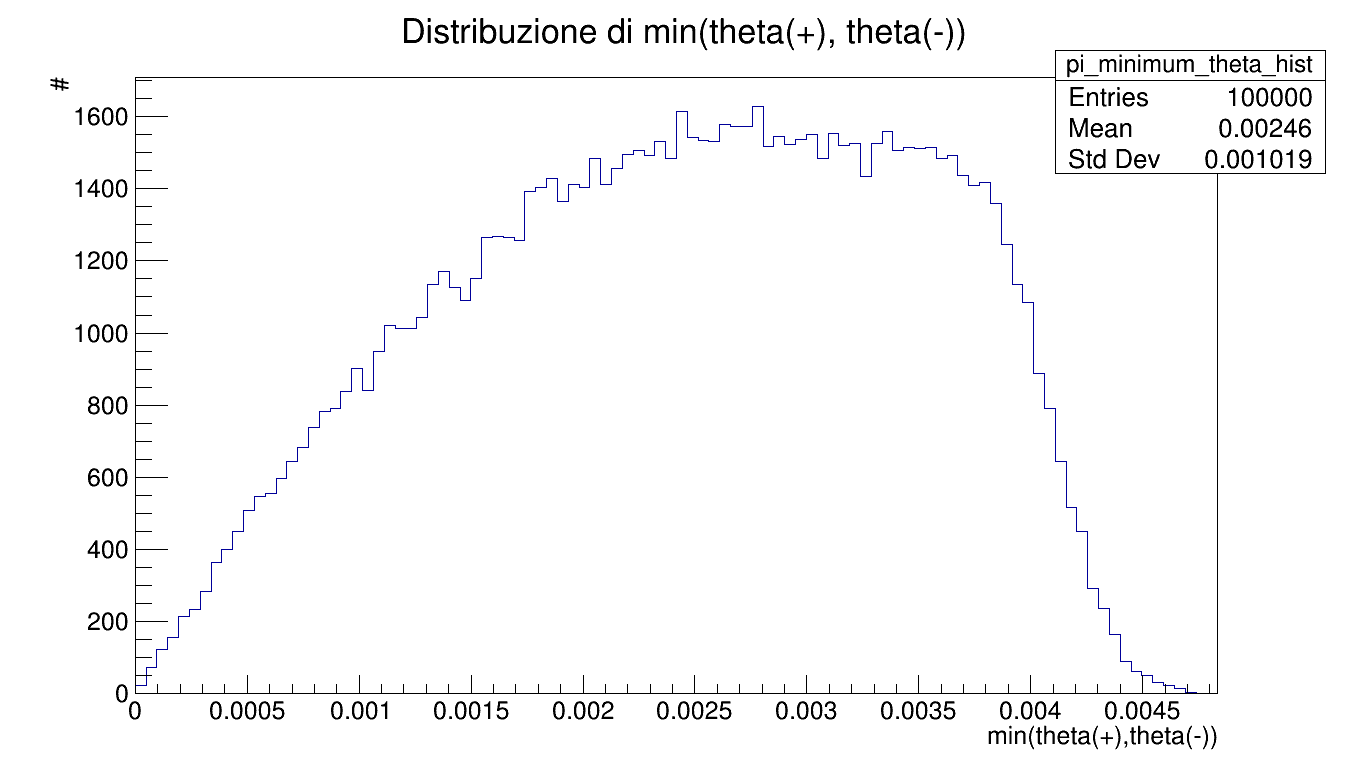
\includegraphics[scale=0.3]{gen_mintheta} 
		\caption{Distribuzione di $min(\theta^+, \theta^-)$. Il massimo di questa distribuzione determina fino a quale z i decadimenti sono visibili(sez.\ref{subsec:raggio_interno}).}
		\label{fig:gen_mintheta}
	\end{center}
\end{figure}

\begin{figure}
	\begin{center}
		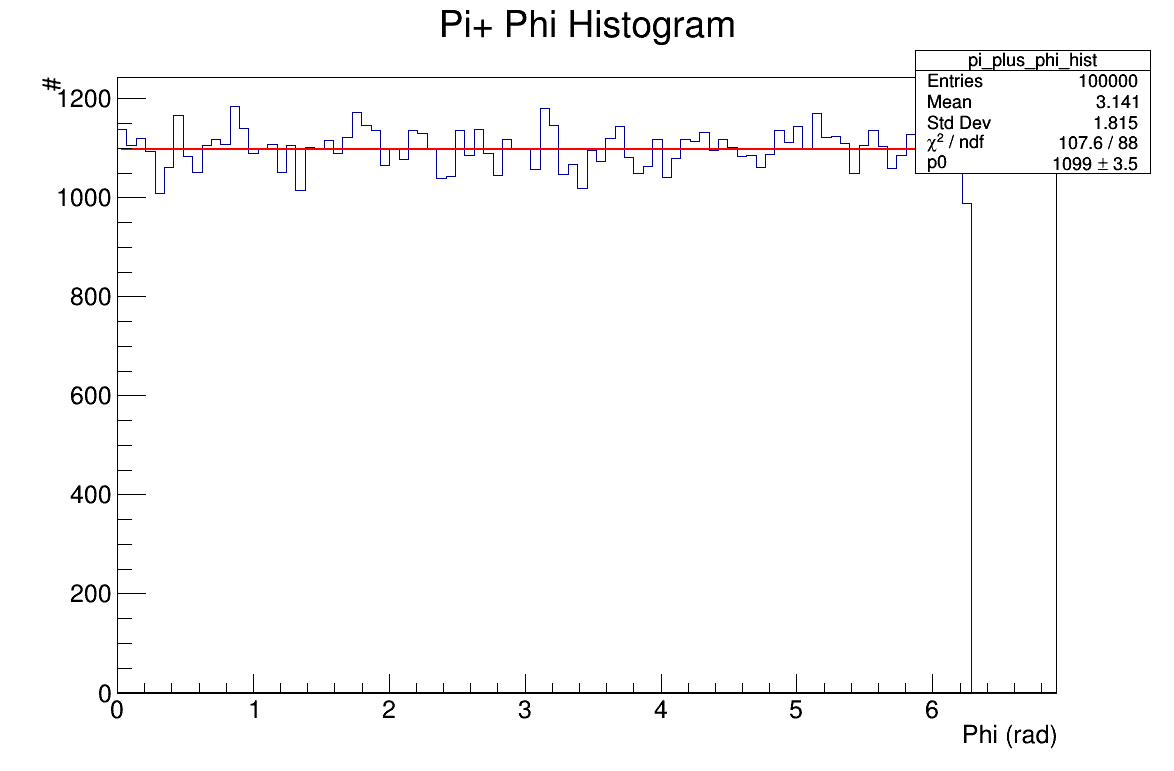
\includegraphics[scale=0.3]{gen_phi} 
		\caption{Distribuzione dell'angolo $\phi$ nel caso del $\pi^+$. Essendo quest'angolo invariato dopo il boost, la distribuzione risulta uniforme tra $0$ e $2\pi$. In figura è mostrato il fit della funzione costante. Nel caso del $\pi^-$ la distribuzione è analoga.}
		\label{fig:gen_phi}
	\end{center}
\end{figure}

\begin{figure}
	\begin{center}
		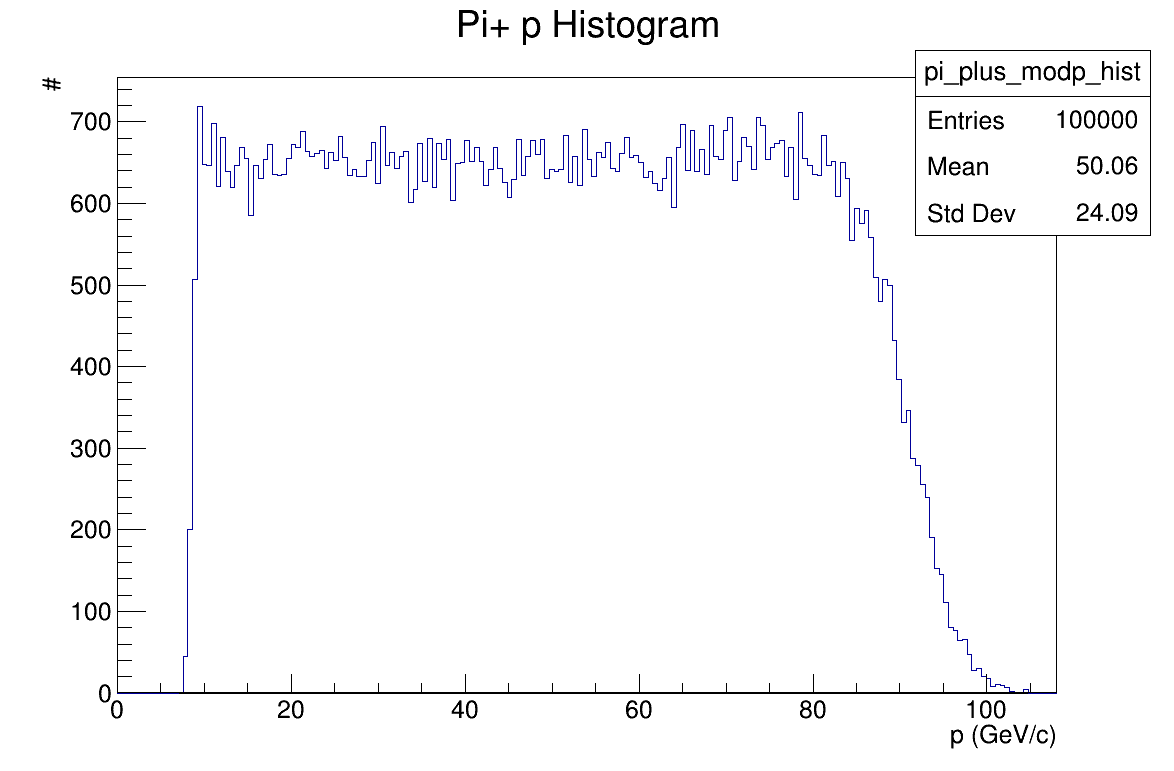
\includegraphics[scale=0.3]{gen_p} 
		\caption{Distribuzione del modulo dell'impulso del $\pi^+$. La distribuzione è limitata inferiormente e superiormente per ragioni cinematiche. Nel caso del $\pi^-$ la distribuzione è analoga.}
		\label{fig:gen_p}
	\end{center}
\end{figure}

\begin{figure}
	\begin{center}
		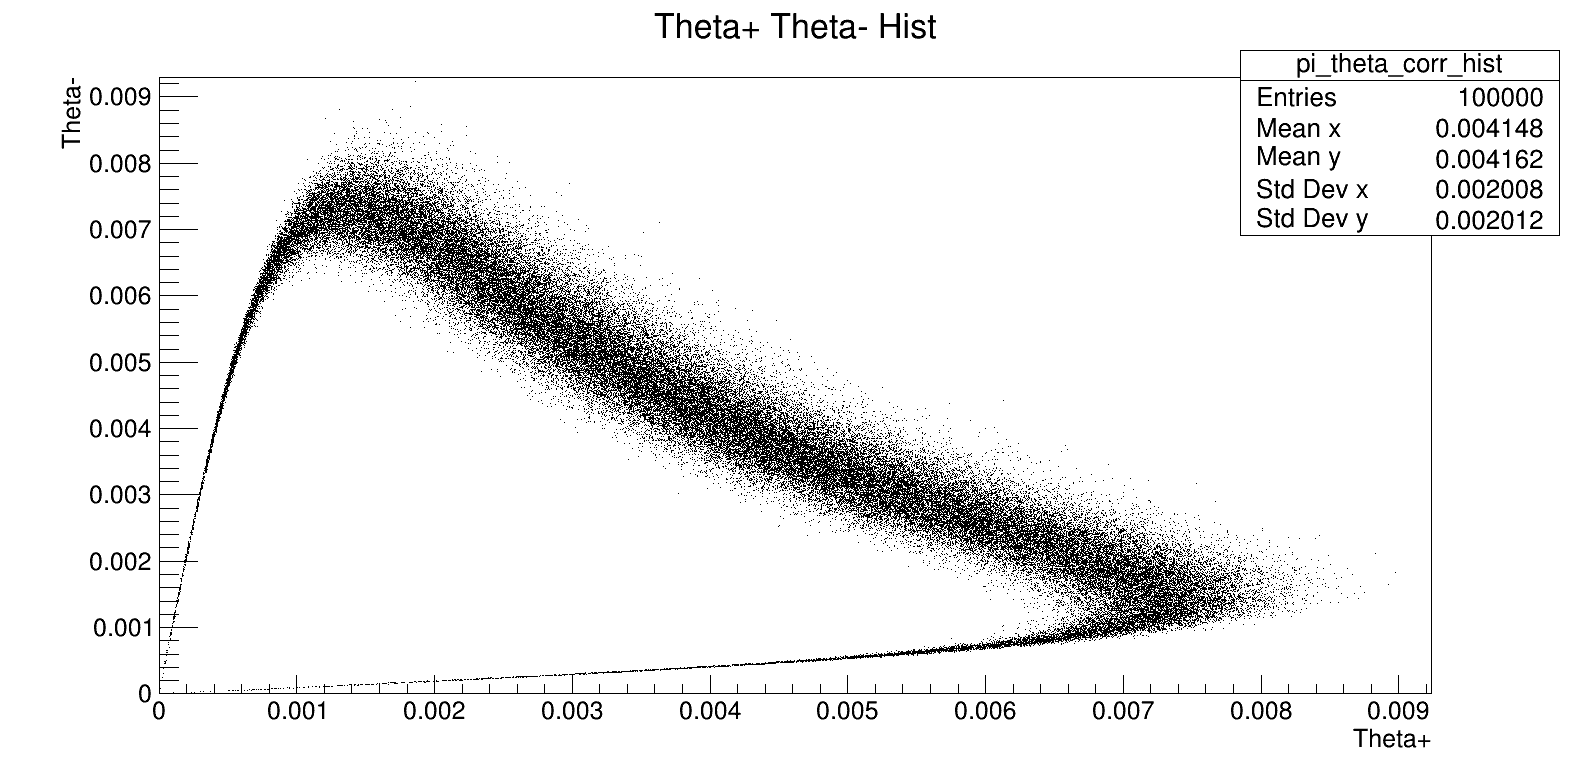
\includegraphics[scale=0.3]{gen_thetatheta} 
		\caption{Correlazione tra gli angoli $\theta$ delle due particelle. Si nota che quando uno è massimo l'altro è piccolo e viceversa.}
		\label{fig:gen_thetatheta}
	\end{center}
\end{figure}

\begin{figure}
	\begin{center}
		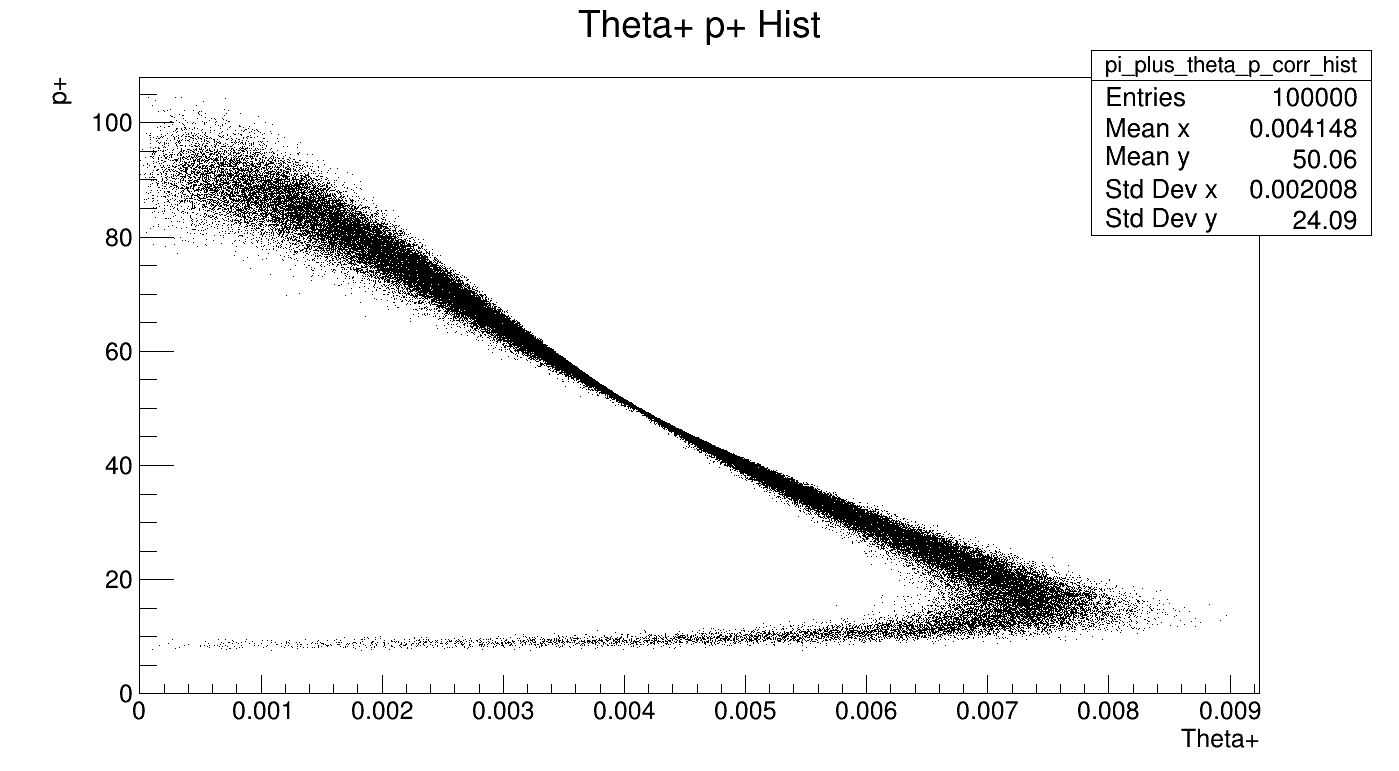
\includegraphics[scale=0.3]{gen_thetap} 
		\caption{Correlazione tra l'angolo $\theta$ del $\pi^+$ e il suo impulso.}
		\label{fig:gen_thetap}
	\end{center}
\end{figure}

Le curve ricalcano il comportamento aspettato e i fit restituiscono un valore di $\chi^2$ accettabile con una fiducia del $1\%$. I parametri ottenuti dai fit sono compatibili con quelli generati.

\section{Simulazione della risposta dei rivelatori} \label{sec:detector}
Il secondo modulo (\textit{Detector}) calcola i punti di passaggio della particella nel rivelatore, escludendo dal salvataggio in memoria quelli che non superano il taglio geometrico imposto dalla struttura del rivelatore. Questo modulo fa uso della classe \textit{B\_event} per simulare l'effetto del campo magnetico e calcolare i punti di passaggio nei piani di rivelatore $3$ e $4$. Ognuno dei quattro rivelatori misura due coordinate per traccia: le misure totali effettuate sono quindi 16.

\subsection{Raggio interno} \label{subsec:raggio_interno}
La scelta del raggio interno si basa su tre aspetti principali:
\begin{itemize}
\item \textit{Larghezza del fascio};
\item \textit{Risoluzione e algoritmi di ricostruzione};
\item \textit{Accettanza}.
\end{itemize}

Per quanto riguarda la \textbf{larghezza del fascio}, essa non è stata presa in considerazione nella simulazione. Ciò nonostante,affinché quest'ultima abbia validità, occorre specificare un raggio interno minimo ragionevole, che collochiamo sugli $8\ cm$. \medskip	

Il secondo aspetto riguarda la \textbf{risoluzione} e gli \textbf{algoritmi di ricostruzione}. Per quanto il fit cinematico utilizzato non faccia uso esclusivo della curvatura della traccia prima e dopo il campo magnetico, nel calcolo dei parametri e nella loro inizializzazione appaiono spesso al denominatore differenze tra le coordinate di due rivelatori. Questo si riflette su un peggioramento del calcolo dei parametri nei casi in cui la differenza delle coordinate sia prossima allo zero, ovvero quando l'angolo $\theta$ delle tracce è piccolo. Prevedere un raggio interno non nullo permette quindi di escludere dall'analisi eventi troppo piatti che comporterebbero un peggioramento complessivo della risoluzione dello spettrometro e/o un eventuale fallimento del fit per tali eventi. \medskip

Il raggio interno non può tuttavia approcciare indefinitamente il massimo teorico (quello per cui solo i decadimenti prodotti nell'origine possono essere rivelati) poiché l'\textbf{accettanza} del sistema tende a zero. \medskip

L'accettanza è definita come la probabilità che un evento venga accettato dal sistema rivelante, dato un avvenuto decadimento. In formule, nel nostro caso: \\
$$
a = P(x_1^{2+} + y_1^{2+} > R_{int}^2 \cap x_1^{2-} + y_1^{2-} > R_{int}^2\ |\ avvenuto\ decadimento)
$$

Questa quantità, nota la configurazione sperimentale, potrebbe essere calcolata teoricamente. Tuttavia, molto raramente questo è possibile e si preferisce misurarla dai dati simulati. Essendo il numero di eventi accettati $r$ distribuiti come una binomiale con numero di prove uguali a $N_{gen}$ (numero di eventi generati) e probabilità di successo $a$, un possibile stimatore per l'accettanza è: 
$$
\hat{a} = \frac{r}{N_{gen}}
$$
$$
Var(\hat{a}) = \frac{a(1-a)}{N_{gen}} \approx \frac{\hat{a}(1-\hat{a})}{N_{gen}}
$$
che risulta essere \textit{unbiased}, di massima verosimiglianza ed efficiente. La sovrastante approssimazione è buona fino a che il numero di eventi accettati è significativamente diverso da zero (o da $N_{gen}$). 

In Fig.\ref{fig:acc_vs_rint} è mostrata la curva di accettanza per il rivelatore, fissate le dimensioni longitudinali a quelle descritte in Sez.\ref{sec:apparato} e al variare del raggio interno.

\begin{figure}
	\begin{center}
		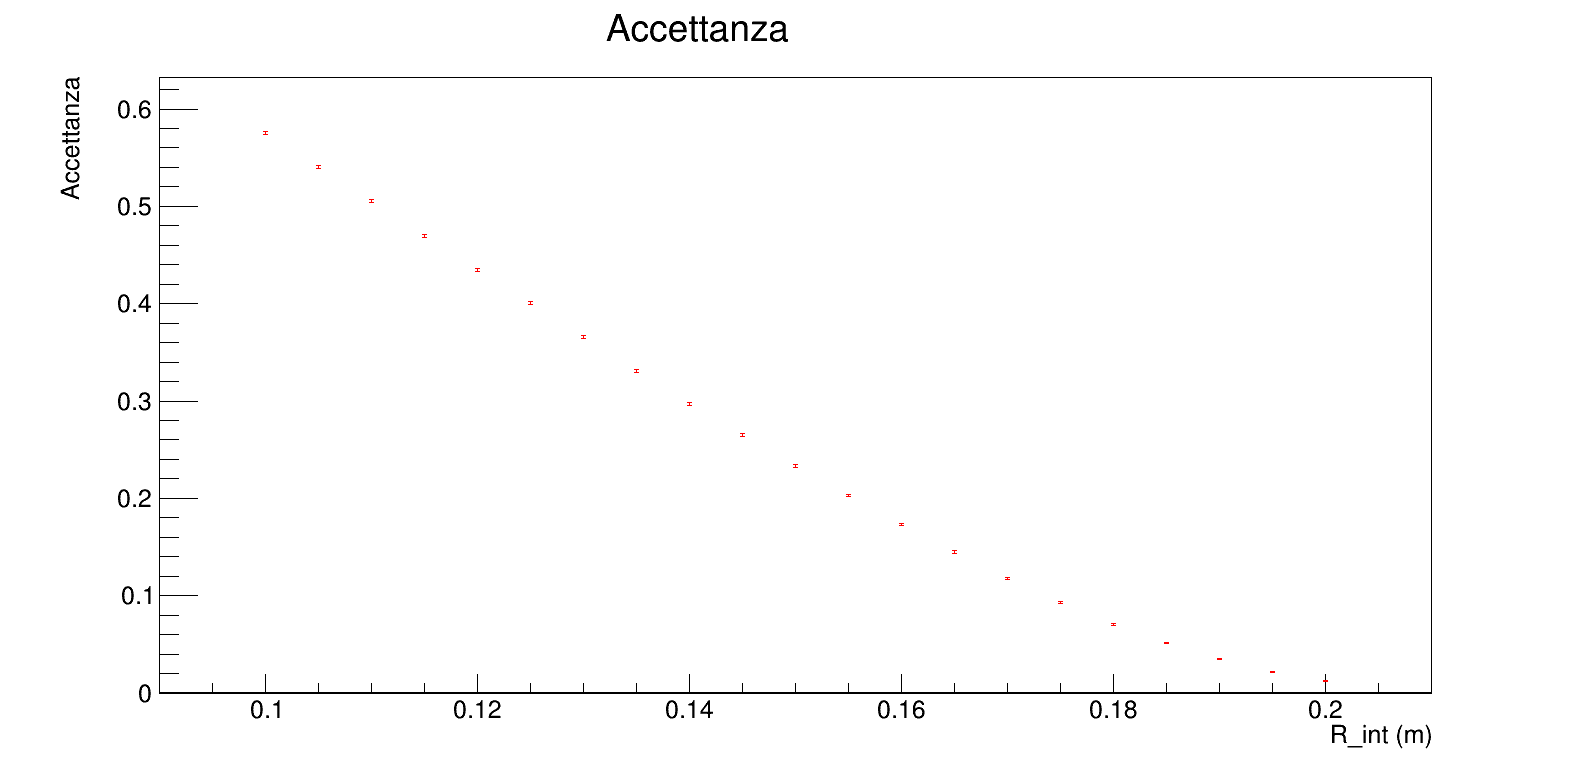
\includegraphics[scale=0.3]{acc_vs_rint} 
		\caption{Accettanza del sistema in funzione del raggio interno del rivelatore $1$.}
		\label{fig:acc_vs_rint}
	\end{center}
\end{figure}

I valori dei raggi mostrati sono stati calcolati, una volta fissato il raggio del primo rivelatore, misurando gli estremi delle distribuzioni delle coordinate degli hit: 
$$
R_{int, i} = min(\sqrt{x_i^{2 \pm} + y_i^{2 \pm}})
$$
$$
R_{ext, i} = max(\sqrt{x_i^{2 \pm} + y_i^{2 \pm}})
$$

Il valore di $R_{int, 1}$, inoltre, determina un valore massimo di z osservabile, che vale: \\
$$
(z_1 - z_{max})\tan{(max(min(\theta^+, \theta^-)))} = R_{int,1} \rightarrow z_{max} \approx 30\ m.
$$

\subsection{Coordinate degli hit: linearità e approssimazione di kick}
Noti gli angoli e il punto di decadimento è possibile calcolare facilmente i punti di arrivo delle tracce sui rivelatori $1$ e $2$. Con riferimento a fig.\ref{fig:apparato_2d}, si ricava:

\begin{equation}
x_{1,2}^{\pm} = (z_{1,2} - z_v) \tan(\theta^{\pm})\cos(\phi^{\pm})
\end{equation}

\begin{equation}
y_{1,2}^{\pm} = (z_{1,2} - z_v) \tan(\theta^{\pm})\sin(\phi^{\pm})
\end{equation}


Per la simulazione dell'effetto del campo magnetico si utilizza un'approssimazione che risulta buona quando $p_k = qB\Delta z << p$ e quando $\cos(\theta) \approx 1$. Nel nostro caso (riferimento a fig.\ref{fig:gen_p})
$$
|p_k| = 105\ MeV/c << p_{min} \approx 15\ GeV/c
$$

In queste condizioni, per una particella incidente a $\theta = 0$, vale
$$
(\vec{p}_{after}-\vec{p}_{before})^2 = (\Delta p)^2 = (F \Delta t)^2 \approx (qB\Delta z)^2
$$
dove $before$ e $after$ si riferiscono al valore assunto prima e dopo il campo magnetico. La precedente relazione, sviluppata usando le approssimazioni porta a
$$
\theta = \frac{p_K}{p}
$$

se $\theta$ non è zero, ma è piccolo, è sufficiente sostituire $\theta \rightarrow \Delta \theta$. 

Usando infine $\Delta \theta \approx \Delta \tan{\theta}$ si ottiene:
$$
\frac{\partial y}{\partial z}|_{after} = \frac{\partial y}{\partial z}|_{before} + sign(q)\frac{|p_k|}{p}
$$
ovvero
\begin{equation}
\frac{y_4^{\pm}-y_3^{\pm}}{z_4-z_3} = \frac{y_2^{\pm}-y_1^{\pm}}{z_2-z_1} + sign(q)\frac{|p_k|}{p}
\label{eq:curvatura}
\end{equation}


mentre le coordinate x rimangono lineari entro queste approssimazioni: 
\begin{equation}
x_{3,4}^{\pm} = (z_{3,4} - z_v) \tan(\theta^{\pm})\cos(\phi^{\pm})
\end{equation}

In queste condizioni l'effetto del campo magnetico è quello di far variare bruscamente la pendenza della traccia con un \textit{kick}, che supponiamo dato nel punto medio tra i rivelatori, dove si colloca il magnete. Imponendo anche che le tracce entrante e uscente si incontrino nel punto medio si ricava:

\begin{equation}
y_3^{\pm} = y_1^{\pm} + (y_2^{\pm}-y_1^{\pm})\frac{z_3-z_1}{z_2-z_1} + \frac{z_3-z_2}{2} sign(q) \frac{|p_k|}{p}
\end{equation}

\subsubsection{Applicazione dello smeering del rivelatore}
Una volta calcolati i punti di passaggio veri della particella, è stato effettuato uno smeering gaussiano di deviazione standard $\sigma_x$ attorno al punto vero (tab.\ref{tab:apparato}, sez.\ref{sec:apparato}).

I risultati sono stati salvati su \textit{ntuple\_det}, che contiene le informazioni fruibili allo sperimentatore.

\section{Ricostruzione dell'evento} \label{sec:reconstruction}

La ricostruzione dell'evento può avvenire su vari livelli di sofisticatezza. Una ricostruzione molto rozza della z di decadimento, per esempio, può essere quella ottenuta invertendo la relazione:
$$
\frac{x_4^{\pm}}{z_4-z_v} = \frac{x_1^{\pm}}{z_1-z_v}
$$

dove sono stati scelti i piani $1$ e $4$ per ridurre l'errore.

Una ricostruzione un po' più sofisticata è rappresentata dalla \textit{Closest Distance of Approach}, ovvero la z corrispondente al punto di minima distanza tra la congiungente degli hit dei rivelatori $1$ e $2$ e l'asse di decadimento. Si ricava in questo caso:
$$
z_{CDA}^{\pm} = z_1 - (z_2-z_1)\frac{x_1^{\pm}(x_2^{\pm}-x_1^{\pm}) + y_1^{\pm}(y_2^{\pm} - y_1^{\pm})}{(x_2^{\pm}-x_1^{\pm})^2-(y_2^{\pm}-y_1^{\pm})^2}
$$

Una ricostruzione migliorata di un fattore $\sqrt{2}$ si può ottenere facilmente semplicemente usando come $z_v$ la media aritmetica dei valori ottenuti per la CDA delle due tracce. \medskip

Per quanto riguarda l'impulso, una prima ricostruzione può essere ottenuta invertendo l'eq.\ref{eq:curvatura} per trovare $p$. In fig.\ref{fig:reco_zCDA},\ref{fig:reco_p_curvatura}, \ref{fig:reco_pk_curvatura} sono mostrate le distribuzioni delle variabili ricostruite meno il loro valor vero. Il valore del $\chi^2$ mostra che la distribuzione scelta per il fit non è compatibile, ma questo non è un problema in quanto non c'è nessun motivo statistico per cui la variabile sia distribuita gaussianamente e il fit serve solo ad estrarre dei parametri sensati. Si noti che la ricostruzione dell'impulso del $K^0$ con la sola curvatura ha portato ad una risoluzione in impulso di circa $9\ GeV/c$, che nel nostro caso non sono sufficienti a descrivere la forma dello spettro che ha una larghezza pari a circa la metà della risoluzione trovata.

\begin{figure}
	\begin{center}
		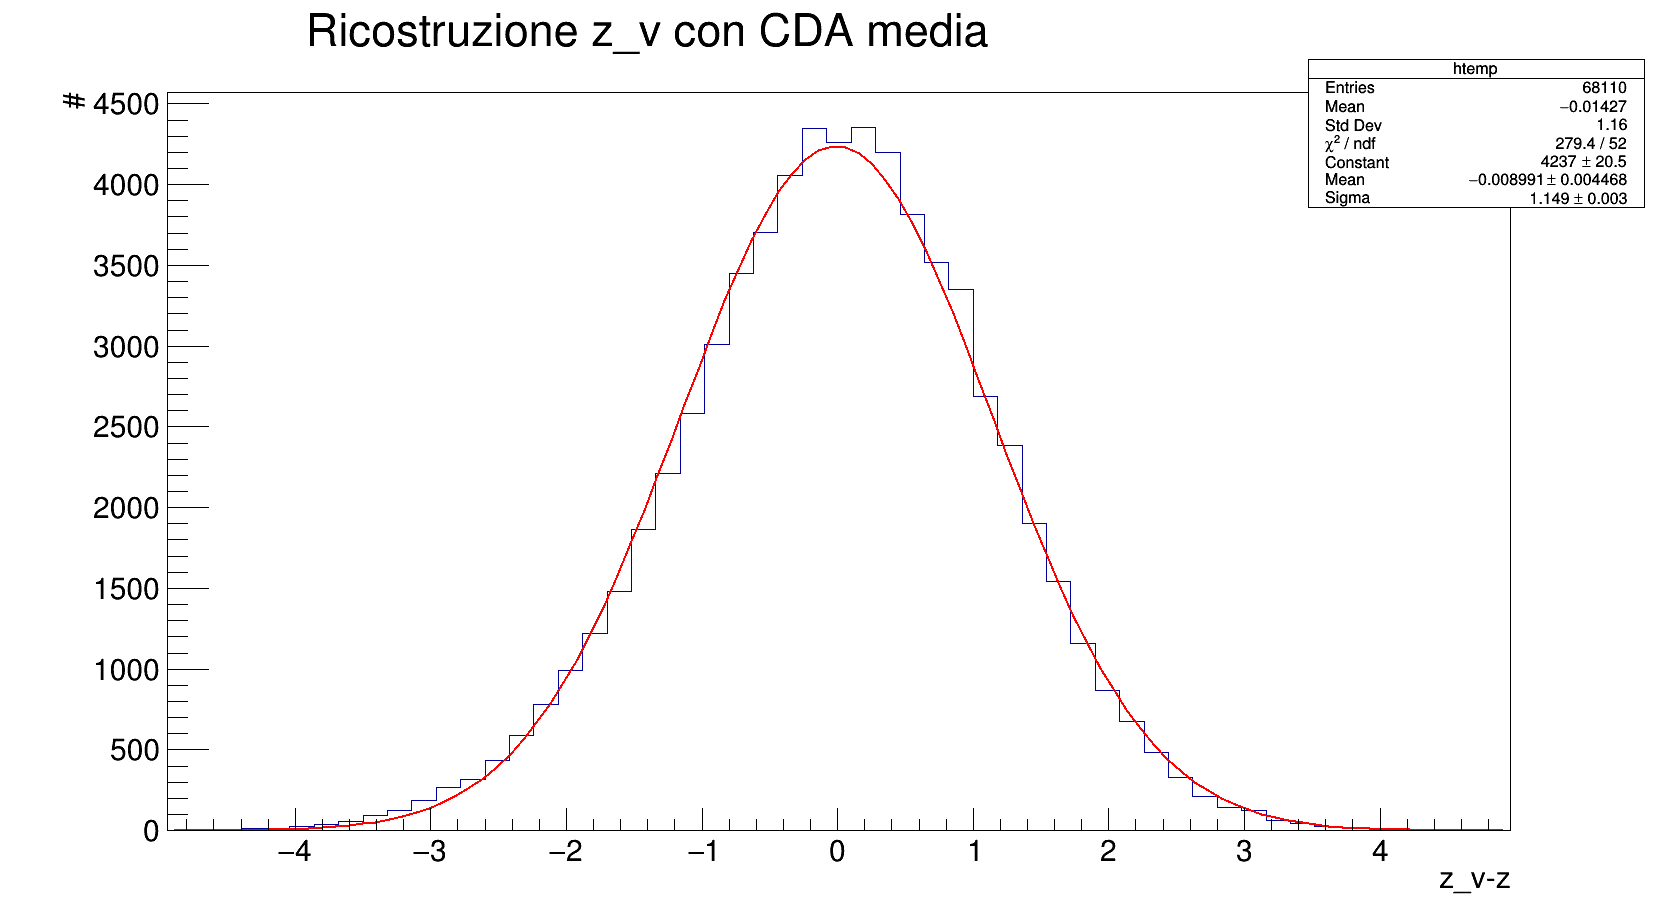
\includegraphics[scale=0.3]{reco_zCDA} 
		\caption{Ricostruzione di $z_v$ con la media delle CDA e fit gaussiano.}
		\label{fig:reco_zCDA}
	\end{center}
\end{figure}

\begin{figure}
	\begin{center}
		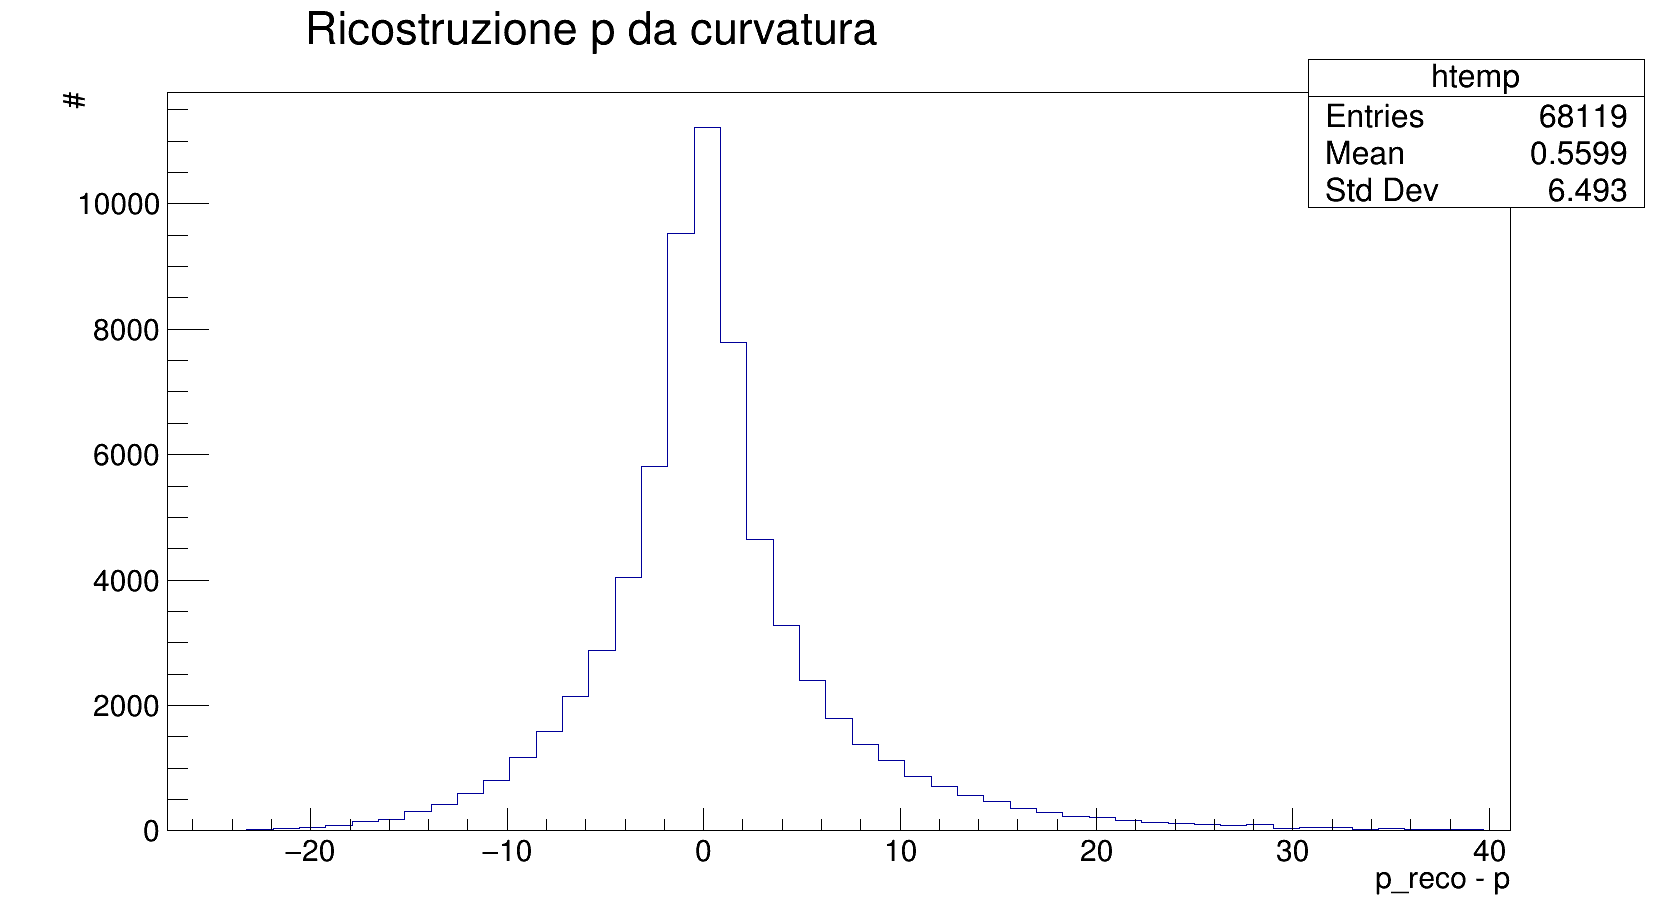
\includegraphics[scale=0.25]{reco_p_curvatura} 
		\caption{Ricostruzione dell'impulso della singola particella con la curvatura.}
		\label{fig:reco_p_curvatura}
	\end{center}
\end{figure}

\begin{figure}
	\begin{center}
		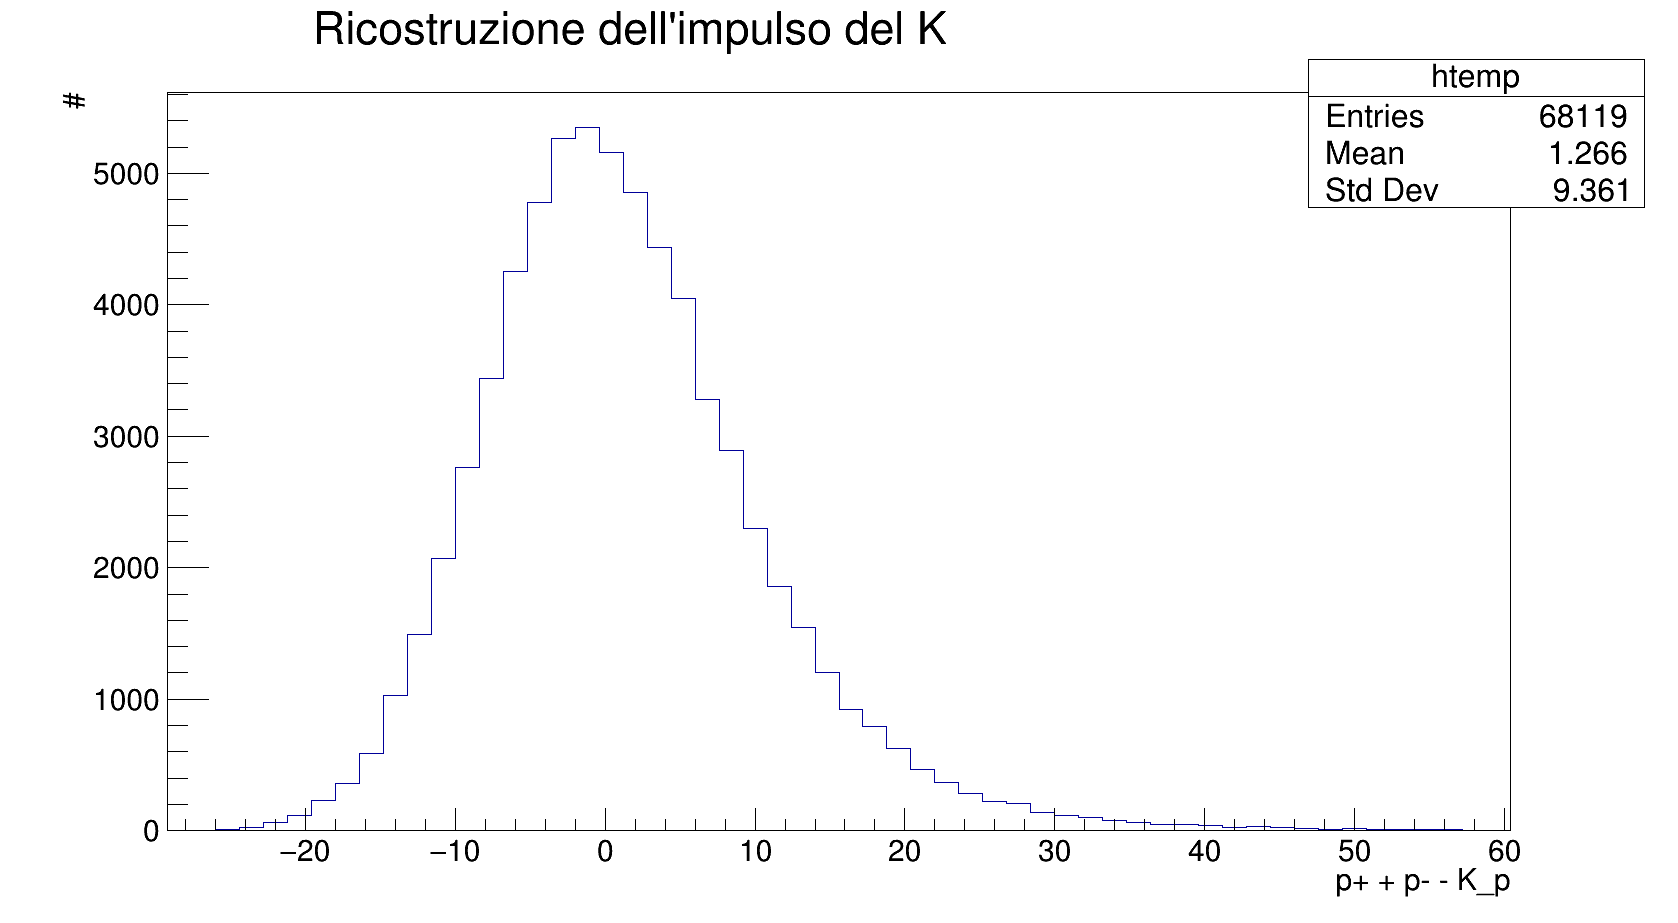
\includegraphics[scale=0.25]{reco_pk_curvatura} 
		\caption{Ricostruzione dell'impulso del K con la curvatura.}
		\label{fig:reco_pk_curvatura}
	\end{center}
\end{figure}

\subsection{La classe IterKinFitP}
Il modo scelto per ricostruire in modo più efficace l'impulso si basa su un metodo iterativo di minimizzazione con N variabili misurate, R parametri non misurati, che rispettano C vincoli scrivibili nella forma $\Phi(x) = 0$. che è stato implementato nella classe \textit{IterKinFitP}. Il metodo si basa sull'uso dei moltiplicatori di Lagrange, nella maniera seguente. Chiamate $x_i$ i valori veri delle N variabili misurate, $\hat{x}_i$ i valori misurati delle variabili\footnote{Nel caso in cui il metodo sia utilizzato iterativamente, $\hat{x}_i$ equivale alle misure solo nella prima iterazione, dopodiché è il generico punto di sviluppo.}, $\lambda_\mu$ i moltiplicatori, , $z_r$ i parametri, $\Phi_\mu$ i vincoli, funzioni delle variabili e dei parametri. Definita una funzione delle variabili e dei moltiplicatori: \\
$$
F = X^2 + \lambda_\mu \Phi_\mu
$$
$$
X^2 = \frac{(x_i - \hat{x}_i)^2}{\sigma_i^2}
$$

Le variabili e i parametri \textit{migliorati} sono trovati minimizzando la funzione $F$ rispetto a $x_i$, $z_r$ e $\lambda_\mu$. Si ottengono infatti
$N+R+C$ equazioni per $N + R+ C$ incognite. Sfortunatamente il punto stazionario della funzione $F$ è tipicamente di sella, il che impedisce l'uso di algoritmi di minimizzazione come ad esempio quello offerto da ROOT nella classe \textit{TMinuit}. Tuttavia, sviluppando al prim'ordine i vincoli attorno ad un punto si può ricavare un sistema lineare risolvibile con un approccio matriciale. Il risultato consiste in due vettori $\Delta_x$ e $\Delta_z$ che andranno aggiunti al punto di sviluppo scelto in precedenza. Nel caso in cui i vincoli siano lineari questo metodo è esatto e il risultato non dipende dal punto di sviluppo scelto, altrimenti dovrà essere iterato fino a che un certo criterio scelto a priori non venga soddisfatto. La scelta del punto iniziale di sviluppo è detta \textit{inizializzazione} e può essere determinante per il successo del metodo nel caso di vincoli non lineari. Nel nostro caso, inoltre, il criterio di convergenza è stato scelto richiedendo che tra un'iterazione e l'altra tutti i parametri e le variabili siano variati, in percentuale, di una quantità inferiore a una certa \textbf{soglia} prefissata. Un metodo che si usa spesso per evitare problemi legati alla non linearità dei vincoli è quello di moltiplicare $\Delta_x$ e $\Delta z$ per un \textbf{coefficiente} minore di 1. Questo potrebbe, per esempio, impedire che il metodo converga su un punto stazionario diverso da quello più vicino all'inizializzazione. \\

La classe \textit{IterKinFitP} implementa questo metodo, richiedendo come inizializzazione il numero di variabili misurate, di parametri e di vincoli, gli errori stimati delle variabili, e le funzioni che restituiscono i vincoli e le loro derivate rispetto alle variabili e ai parametri. Sono stati anche predisposti dei metodi pubblici per modificare ad un valore diverso da quello di default i valori della soglia e del coefficiente di convergenza. Il coefficiente ideale va cercato caso per caso e dipende dall'entità della non linearità e dal tempo di calcolo massimo. \\

Per quanto riguarda la scelta dell'inizializzazione, le variabili vanno inizializzate con le loro misure sperimentali, mentre con i parametri si può normalmente usare una stima ottenuta, ad esempio, dall'inversione di un vincolo, sostituendo alle variabili teoriche quelle misurate. \\

Una volta terminata la minimizzazione, si può calcolare la variabile $X^2$ nelle misure migliorate. Si può dimostrare che nel caso di vincoli lineari questa variabile è distribuita come $\chi^2_{C-R}$. \\
\subsection{Set di vincoli scelti}
Nel caso dello spettrometro, abbiamo scelto vari set di vincoli per confrontare le risoluzioni ottenute e i tempi di calcolo necessari. Un problema a più tracce come quello studiato in questo progetto si può affrontare almeno in due modi:
\begin{itemize}
\item Approccio a singola traccia;
\item Approccio esaustivo.
\end{itemize}

Nell'approccio a singola traccia si esegue il fit su ogni traccia: ha il vantaggio di essere facilmente applicabile al caso generico di un numero arbitrario di tracce, ma, almeno nella sua versione più semplice, non può beneficiare dell'aggiunta di quei vincoli che nascono dalla correlazione tra le tracce (es. stesso vertice), a scapito della risoluzione ottenuta. \\
Nell'approccio esaustivo, anziché eseguire un fit per ogni traccia si esegue un unico fit su tutte le tracce. Questo ha il vantaggio di poter tenere conto di più vincoli e quindi di migliorare la risoluzione sulle variabili e i parametri, ma deve essere scritto caso per caso e comporta una maggiore onerosità computazionale. \medskip

Abbiamo deciso di confrontare l'approccio a singola traccia con quattro diversi set di vincoli in approccio esaustivo. A seguire sono elencati i 15 possibili vincoli con cui si può effettuare il fit cinematico, i primi 12 lineari e gli ultimi 3 non lineari.

\begin{equation}
x_1^{\pm} (z_{2,3,4} - z_v) - x_{2,3,4}^{\pm} (z_1 - z_v) = 0
\end{equation}

\begin{equation}
y_1^{\pm} (z_{2} - z_v) - y_{2}^{\pm} (z_1 - z_v) = 0
\end{equation}

\begin{equation}
y_3^{\pm} - y_1^{\pm} - (y_2^{\pm}-y_1^{\pm})\frac{z_3-z_1}{z_2-z_1} \mp \frac{z_3-z_2}{2} \frac{|p_k|}{p^{\pm}} = 0
\label{eq:curvaturay3}
\end{equation}

\begin{equation}
\frac{y_4^{\pm}-y_3^{\pm}}{z_4-z_3} - \frac{y_2^{\pm}-y_1^{\pm}}{z_2-z_1} \mp \frac{|p_k|}{p^{\pm}} = 0
\end{equation}

\begin{align}
\begin{split}
&(-\frac{1}{p^-}) (x_2^+ - x_1^+) \sqrt{(x_2^- - x_1^-)^2 + (y_2^- - y_1^-)^2 + (z_2 - z_1)^2} + \\
& - (\frac{1}{p^+}) (x_2^- - x_1^-) \sqrt{(x_2^+ - x_1^+)^2 + (y_2^+ - y_1^+)^2 + (z_2 - z_1)^2} = 0 
\end{split}
\end{align}

\begin{align}
\begin{split}
&(-\frac{1}{p^-}) (y_2^+ - y_1^+) \sqrt{(x_2^- - x_1^-)^2 + (y_2^- - y_1^-)^2 + (z_2 - z_1)^2} + \\
& - (\frac{1}{p^+}) (y_2^- - y_1^-) \sqrt{(x_2^+ - x_1^+)^2 + (y_2^+ - y_1^+)^2 + (z_2 - z_1)^2} = 0 
\end{split}
\end{align}

\begin{align}
\begin{split}
&m_\pi^2 + \sqrt{p^{2+} + m_\pi^2}\sqrt{p^{2-} + m_\pi^2} + p^{2+} \frac{(x_2^+ - x_1^+)^2 + (y_2^+ - y_1^+)^2}{(x_2^+ - x_1^+)^2 + (y_2^+ - y_1^+)^2 + (z_2 - z_1)^2} + \\
& -p^+ p^- \frac{(z_2-z_1)^2}{\sqrt{(x_2^+ - x_1^+)^2 + (y_2^+ - y_1^+)^2 + (z_2 - z_1)^2}\sqrt{(x_2^- - x_1^-)^2 + (y_2^- - y_1^-)^2 + (z_2 - z_1)^2}} + \\
& -m_K^2/2 = 0
\end{split}
\end{align}

Le prime due equazioni rappresentano 4 vincoli per ogni traccia e non sono altro che l'imposizione che le due tracce siano originate dallo stesso punto dell'asse z. Le seguenti due equazioni sono legate all'effetto del campo magnetico: la terza è il vincolo che il kick avvenga nel punto medio tra i rivelatori $2$ e $3$, mentre la quarta è il già visto vincolo di curvatura. \\
Delle seguenti equazioni, le prime due vincolano la componente trasversa dell'impulso totale ad essere zero ($\vec{p}^T = 0$), mentre l'ultima è il vincolo che la massa invariante dei due $\pi$ sia la massa del $K^0$.

Per quanto riguarda i parametri, sono 4 nel caso dell'approccio a singola traccia ($z_v^+$, $z_v^-$, $1/p^+$, $-1/p^-$)\footnote{Il segno meno per l'ultimo parametro è stato scelto in modo da eliminare il $\mp$ dei vincoli di curvatura}, e tre nel caso di approccio esaustivo ($z_v, 1/p^+, -1/p^-$). L'inizializzazione scelta è stata la CDA per quanto riguarda la $z_v$, e l'inversione del vincolo di curvatura per quanto riguarda gli impulsi.

In tab.\ref{tab:set_vincoli} sono specificati i set di vincoli scelti con cui è stata effettuata la ricostruzione.

\begin{table} [h!]
\centering
\begin{tabular}{||p {2.0 cm}|p {4.5 cm}||}
\hline
\textbf{ID set} & \textbf{Tipo} \\
\hline \hline
1 & S + LIN + CURV \\
\hline
2 & E + LIN + CURV \\
\hline
3 & E + LIN + CURV + PT \\
\hline
4 & E + LIN + CURV + MK \\
\hline
5 & E + LIN + CURV + PT + MK \\
\hline \hline
\end{tabular} 
\caption{Lista dei set di vincoli scelti per confrontare l'efficacia di ricostruzione. S = approccio singola traccia; E = approccio esaustivo; LIN = vincoli di linearità della traccia; CURV = vincoli di curvatura; PT = vincoli di annullamento del vettore di impulso trasverso; MK = vincolo di massa invariante.}
\label{tab:set_vincoli}
\end{table}

\subsection{Risultati}
In tutti i casi il numero di eventi generati scelto è stato $10^5$. Per tutti i fit cinematici sono state impostate le soglie uguali a $10^{-5}$ e i coefficienti di convergenza a $0.5$, a parte nel caso del set numero 5, in cui molti eventi superavano il numero massimo di iterazioni e si è dunque preferito usare una soglia $10^{-6}$ e un coefficiente di convergenza $0.2$.

Alcuni dei grafici dei risultati sono riportati in appendice, sez.\ref{subsec:grafici}. In diversi casi, unitamente ai grafici, è anche presente un fit. Con eccezione dei grafici del $\chi^2$ si tratta di un fit gaussiano, che non ha nessun fondamento statistico se non quello di confrontare la curva ottenuta con una curva nota e rendere più evidenti eventuali asimmetrie. Tra i risultati sono riportati gli istogrammi della risoluzione della $x_1^+$, a titolo di esempio, che mostra per tutti i set di vincoli un miglioramento della misura rispetto a quella del rivelatore e una deformazione della curva gaussiana in una più piccata. Per quanto riguarda la ricostruzione del vertice, la distribuzione appare leggermente asimmetrica verso sinistra, ovvero succede più spesso che $z_{reco} < z$ che il viceversa. Questo è dovuto al fatto che un errore nella determinazione delle coordinate produce un errore asimmetrico sulla z, privilegiando le z piccole a quelle grandi. Per quanto riguarda il $\chi^2$, si noti che nei set di vincoli 1 e 2, dove si utilizzano solo vincoli lineari, il fit è compatibile con la distribuzione attesa, mentre si osserva una deviazione significativa dalla distribuzione aspettata quando si introducono vincoli non lineari. Questo è in linea con quanto atteso. La risoluzione dell'impulso, risultato principale della simulazione, è progressivamente migliore quanti più vincoli si sfruttano, come aspettato. Dal confronto tra le risoluzioni ottenute nei set di vincoli 3, 4, 5 si nota che risulta particolarmente importante il vincolo di massa invariante. Nei grafici è anche riportato il grafico della massa invariante per il set di vincoli 2, in cui non si utilizzano vincoli per l'impulso. Per ricostruire adeguatamente lo spettro del $K^0$, che ha una larghezza di $5\ GeV/c$, occorre dunque scegliere un algoritmo di ricostruzione che abbia una risoluzione significativamente inferiore. Con un apparato sperimentale come quello simulato si è in grado di trovare una stima della larghezza dello spettro con un errore del $1\%$ utilizzando il set di vincoli numero 5.

\'E stata anche studiata la dipendenza della risoluzione dello spettrometro dal raggio interno del primo rivelatore: non sono state riscontrate dipendenze apprezzabili. La scelta del raggio interno è quindi stata quella riportata in tab.\ref{tab:apparato}, ovvero quella minima per una ragionevole larghezza di fascio, affinché l'accettanza del sistema sia massima. In tab.\ref{tab:risultati} sono riportate le risoluzioni per i vari set di vincoli e il tempo di calcolo necessario per la ricostruzione di un evento. Quest'ultimo è ovviamente dipendente dalla macchina su cui si esegue il calcolo, ma i rapporti tra i tempi sono indicativi dell'onerosità computazionale richiesta.

\begin{table} [h!]
\centering
\begin{tabular}{||p {1.3 cm}|p {2.5 cm} | p {1.7 cm}||}
\hline
\textbf{ID set} & \textbf{Risoluzione(GeV/c)} & \textbf{Tempo(s)/ev} \\
\hline \hline
1 & 6.9 & 0.0003 \\
\hline
2 & 5.9 & 0.0005 \\
\hline
3 & 4.8 & 0.0006 \\
\hline
4 & 2.3 & 0.017 \\
\hline
5 & 1.0 & 0.04 \\
\hline
3 riv. & 1.9 & 0.015 \\
\hline \hline
\end{tabular} 
\caption{Tabella riassuntiva dei risultati della ricostruzione per i vari set di vincoli. Per il calcolo dei tempi, la soglia di convergenza del fit cinematico è stata impostata a $10^{-5}$ e il coefficiente di convergenza a $0.5$.}
\label{tab:risultati}
\end{table}



\subsection{Problema combinatorio}
Un problema che si incontra sempre sperimentalmente quando si vuole ricostruire un evento a più tracce è quello dovuto all'individuazione degli hit facenti parte della stessa traccia. Nel caso analizzato in questa simulazione questo problema non è particolarmente ostico perché ci sono solo due tracce . Il problema è stato risolto utilizzando il fit cinematico iterativo su tutte le possibili combinazioni (8, perché delle $2^4$ totali la metà sono ripetute) e cercando quella con il $\chi^2$ inferiore. Usando il set di vincoli numero 2 per quest'analisi è stato ottenuto un rate di successi del 100\% su 5000 eventi generati. \'E stato quindi possibile calcolare un limite superiore per il fondo di questi eventi:
$$
B/S < 6\cdot 10^{-4}, 95\% CL
$$

\subsection{Misura della risoluzione con tre rivelatori}
Per completezza è stato anche analizzato il caso in cui il quarto rivelatore non sia inserito. In questo caso si è scelto di procedere utilizzando tutte le informazioni possibili, e quindi un fit cinematico di tipo esaustivo con tutti i vincoli. Per quanto riguarda l'inizializzazione, si è utilizzata la CDA per la $z_v$, mentre per l'impulso, non potendo più usare il secondo vincolo di curvatura, si è utilizzato il primo (eq.\ref{eq:curvaturay3}). In questo caso l'inizializzazione dell'impulso risulta avere segno errato circa il 4\% delle volte, ma questo problema si può parzialmente risolvere tagliando dall'analisi tutti gli eventi in cui almeno uno dei momenti ricostruiti sia negativo. \'E stato invece riscontrato che nell'1\% dei casi il fit non converge. Rispetto al caso di 4 rivelatori, quindi, sono stati effettuati alcuni tagli sugli eventi. Si è verificato che tagliando gli eventi con $\chi^2 > 50$ o con almeno un impulso negativo si perde il 5$\%$ degli eventi ma si ottiene una buona risoluzione sull'impulso del $K^0$ pari a $2\ GeV/c$, che è comunque circa il doppio rispetto alla migliore ottenuta con 4 rivelatori.


\section{Conclusioni} \label{sec:conclusioni}
La simulazione effettuata è da considerarsi fondamentalmente uno studio sulle tecniche di ricostruzione. Il processo fisico è infatti estremamente semplificato rispetto a quello della realtà sperimentale, soprattutto perché non sono stati considerati fondi nè causati da altri decadimenti, né da impurità del fascio. L'uso dei fit cinematici ha permesso di migliorare di un fattore circa 10 la risoluzione ottenuta dal calcolo diretto della curvatura. La risoluzione migliore ottenuta è infatti di circa $1.0\ GeV/c$, rispetto a quella della ricostruzione diretta di $9.3\ GeV/c$. 

\newpage

\section{Appendice}
\subsection{Grafici dei risultati} \label{subsec:grafici}

\begin{figure} [h!]
	\begin{center}
		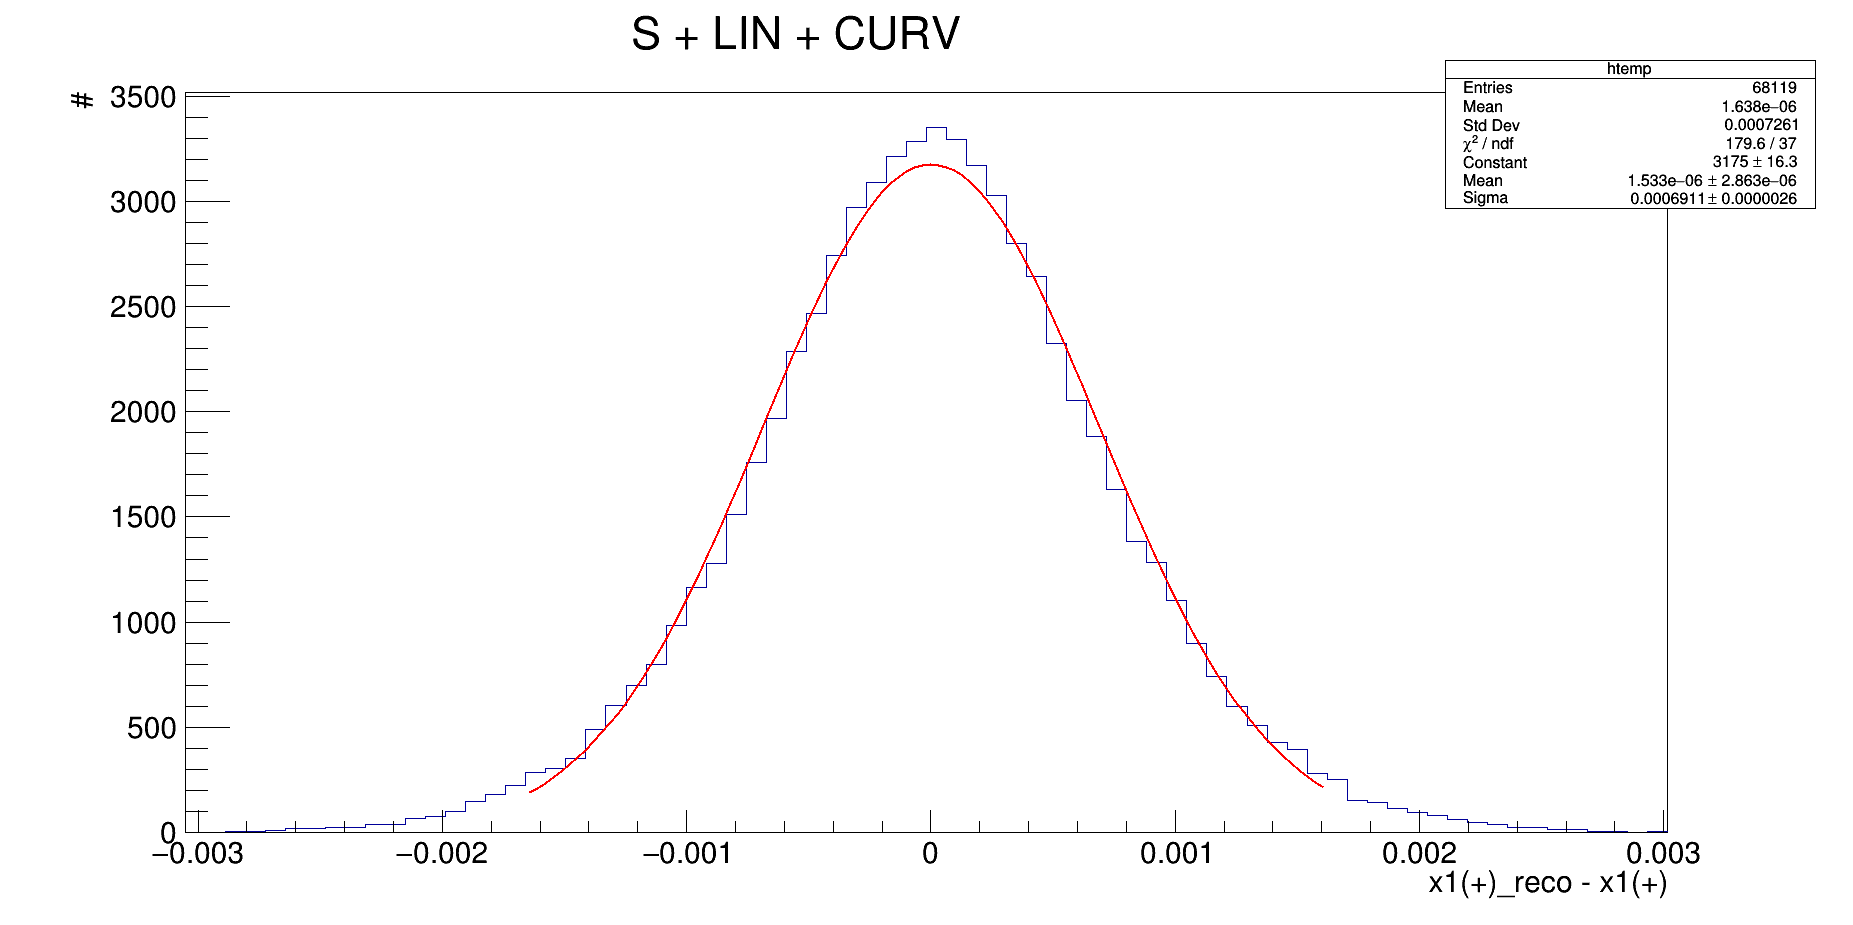
\includegraphics[scale=0.25]{set_1_x} 
		\caption{Risoluzione di $x_1^+$ con il set di vincoli numero 1. La risoluzione è migliorata rispetto a quella del rivelatore (0.001).}
		\label{fig:set_1_x}
	\end{center}
\end{figure}

\begin{figure} [h!]
	\begin{center}
		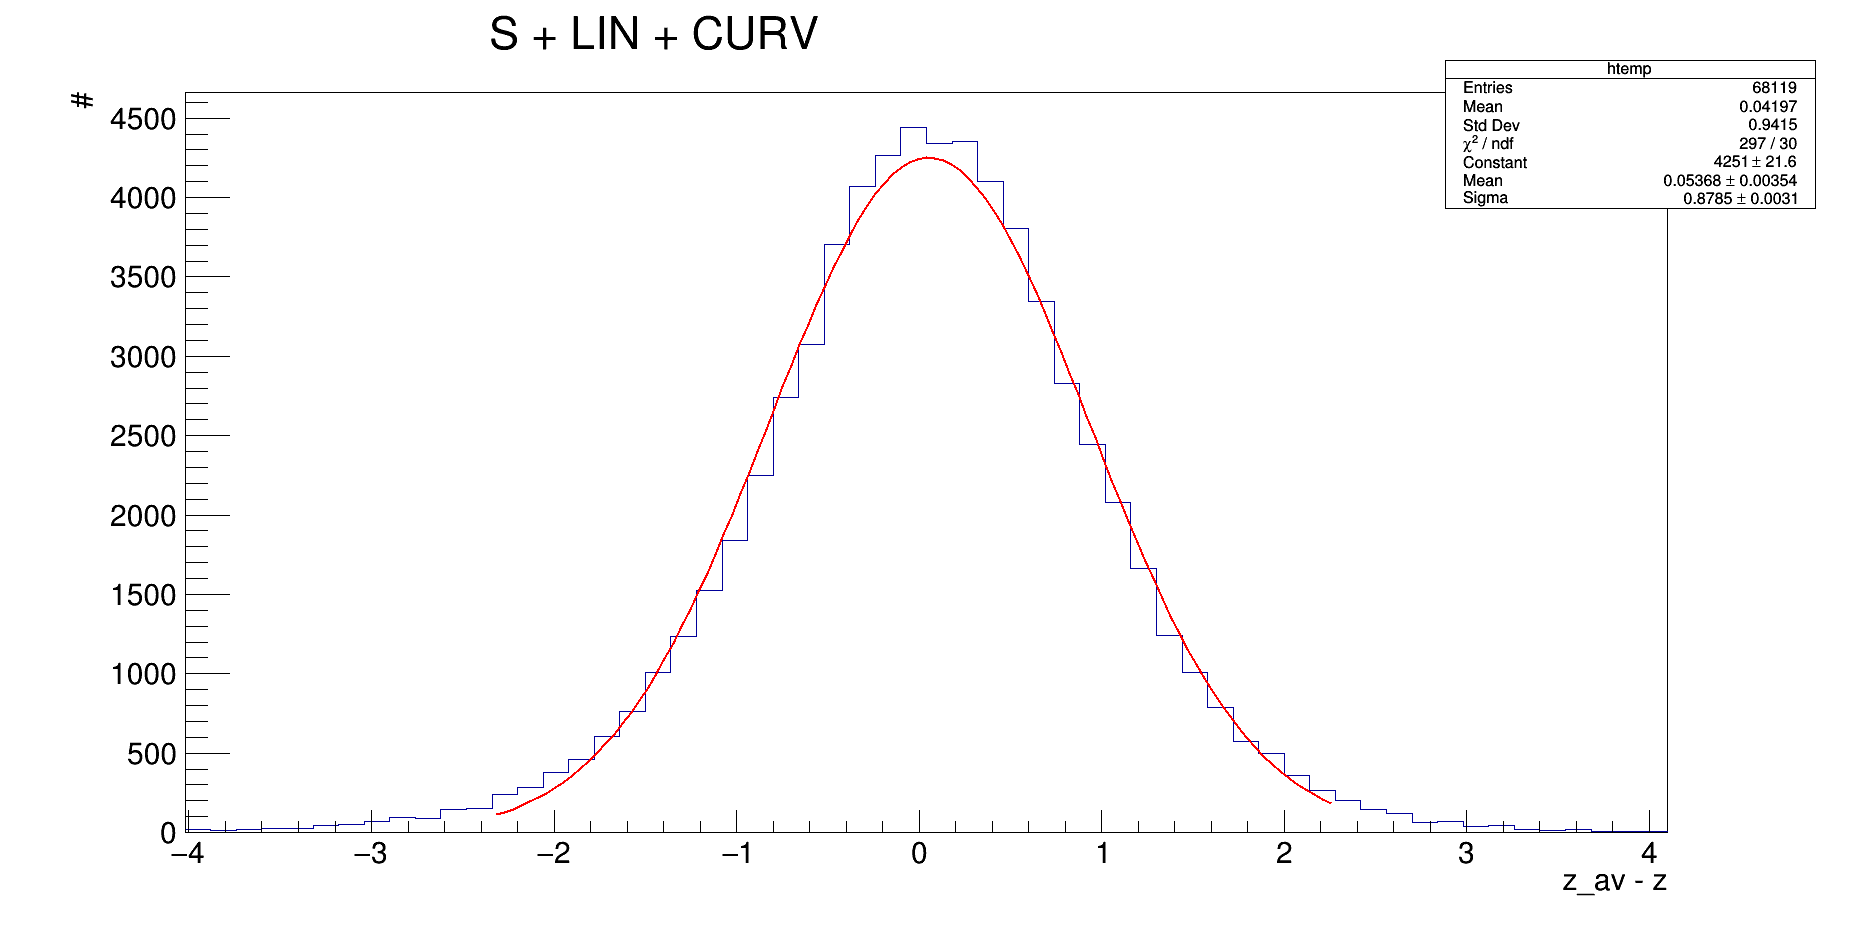
\includegraphics[scale=0.25]{set_1_z} 
		\caption{Risoluzione di $z_v^+$ con il set di vincoli numero 1. Per migliorare la risoluzione si è usata la variabile $0.5(z^+_{reco}+z^-_{reco})$.}
		\label{fig:set_1_z}
	\end{center}
\end{figure}

\begin{figure} [h!]
	\begin{center}
		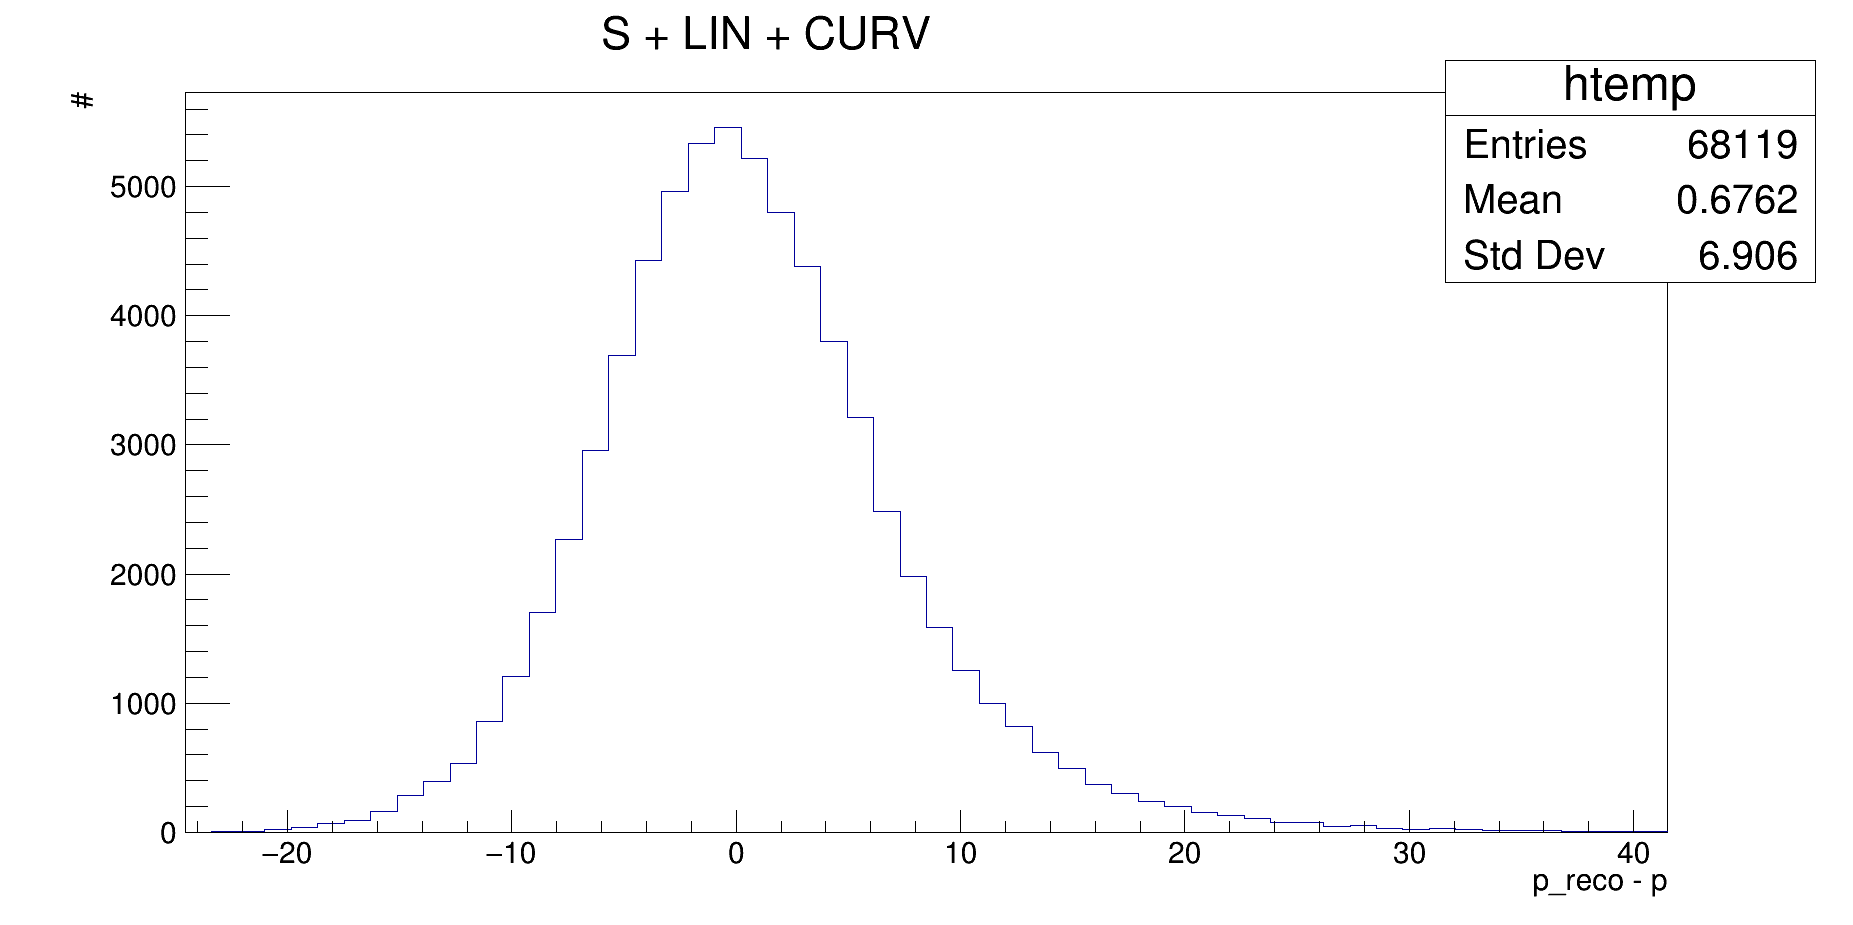
\includegraphics[scale=0.25]{set_1_p} 
		\caption{Risoluzione dell'impulso del $K^0$ con il set di vincoli numero 1. L'impulso è calcolato come $p^+ + p^-$, la parte angolare apporta un contributo trascurabile, a questa risoluzione.}
		\label{fig:set_1_p}
	\end{center}
\end{figure}

\begin{figure} [h!]
	\begin{center}
		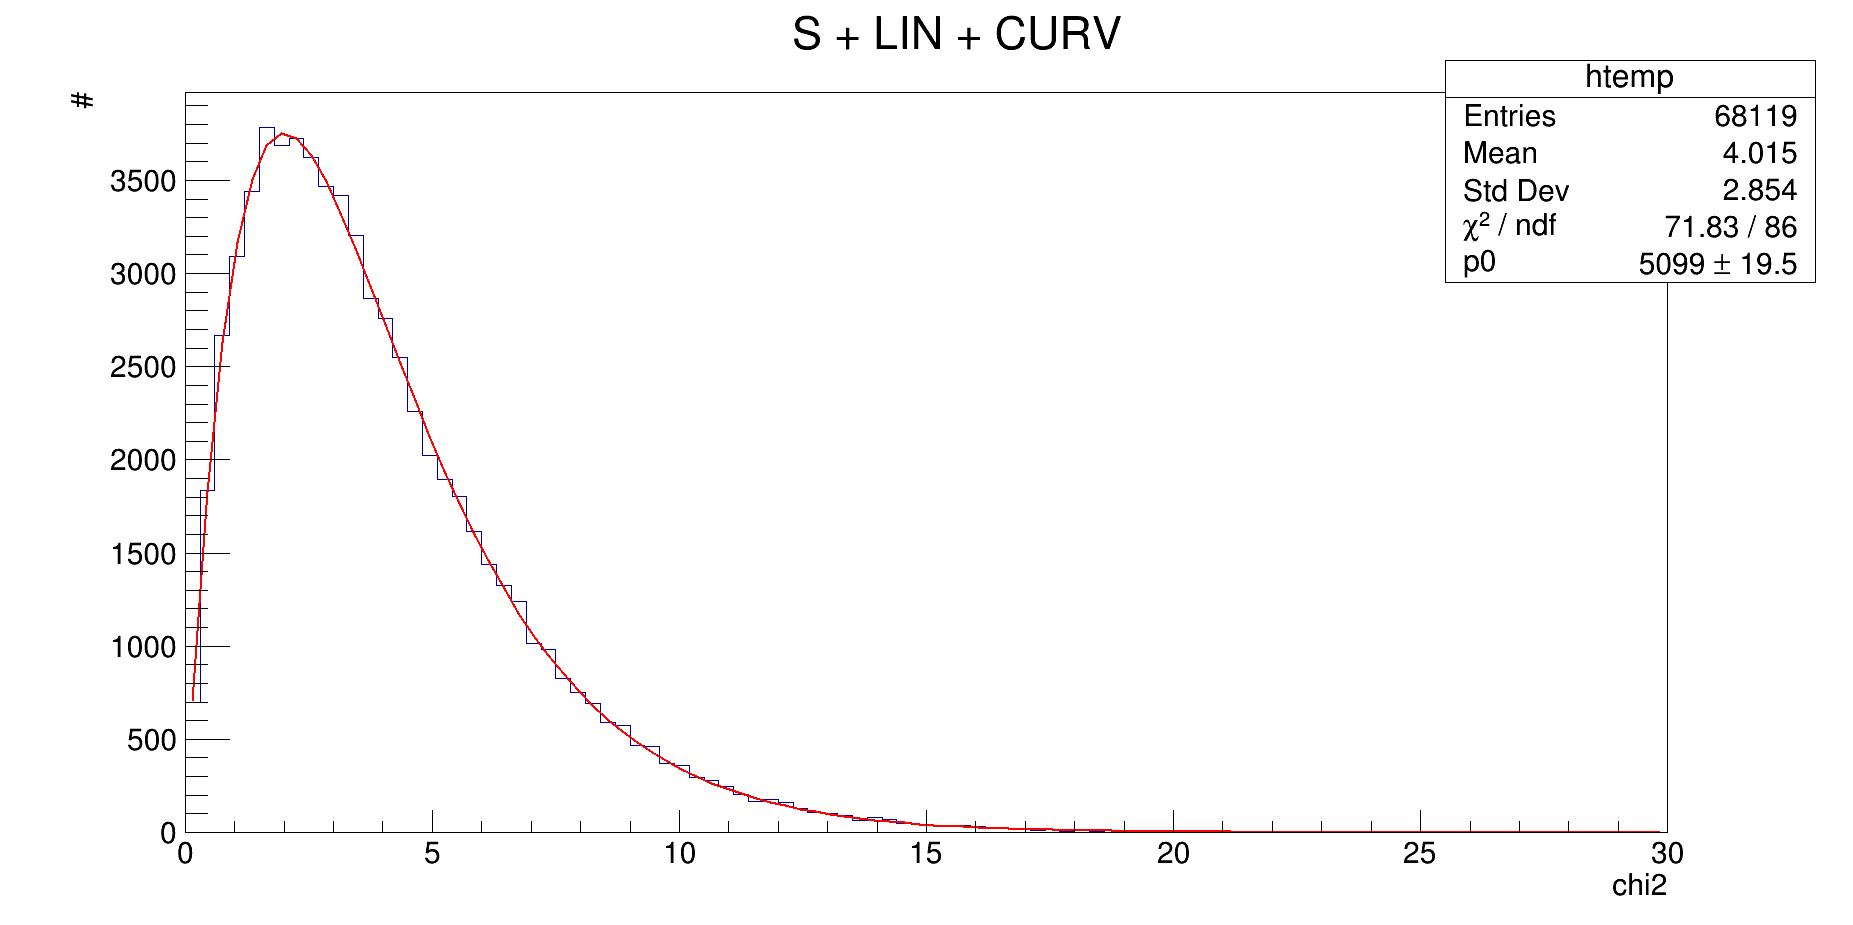
\includegraphics[scale=0.25]{set_1_chi2} 
		\caption{Distribuzione della funzione $X^{2,+}$ e fit con una distribuzione $\chi^2_4$}
		\label{fig:set_1_chi2}
	\end{center}
\end{figure}

\begin{figure} [h!]
	\begin{center}
		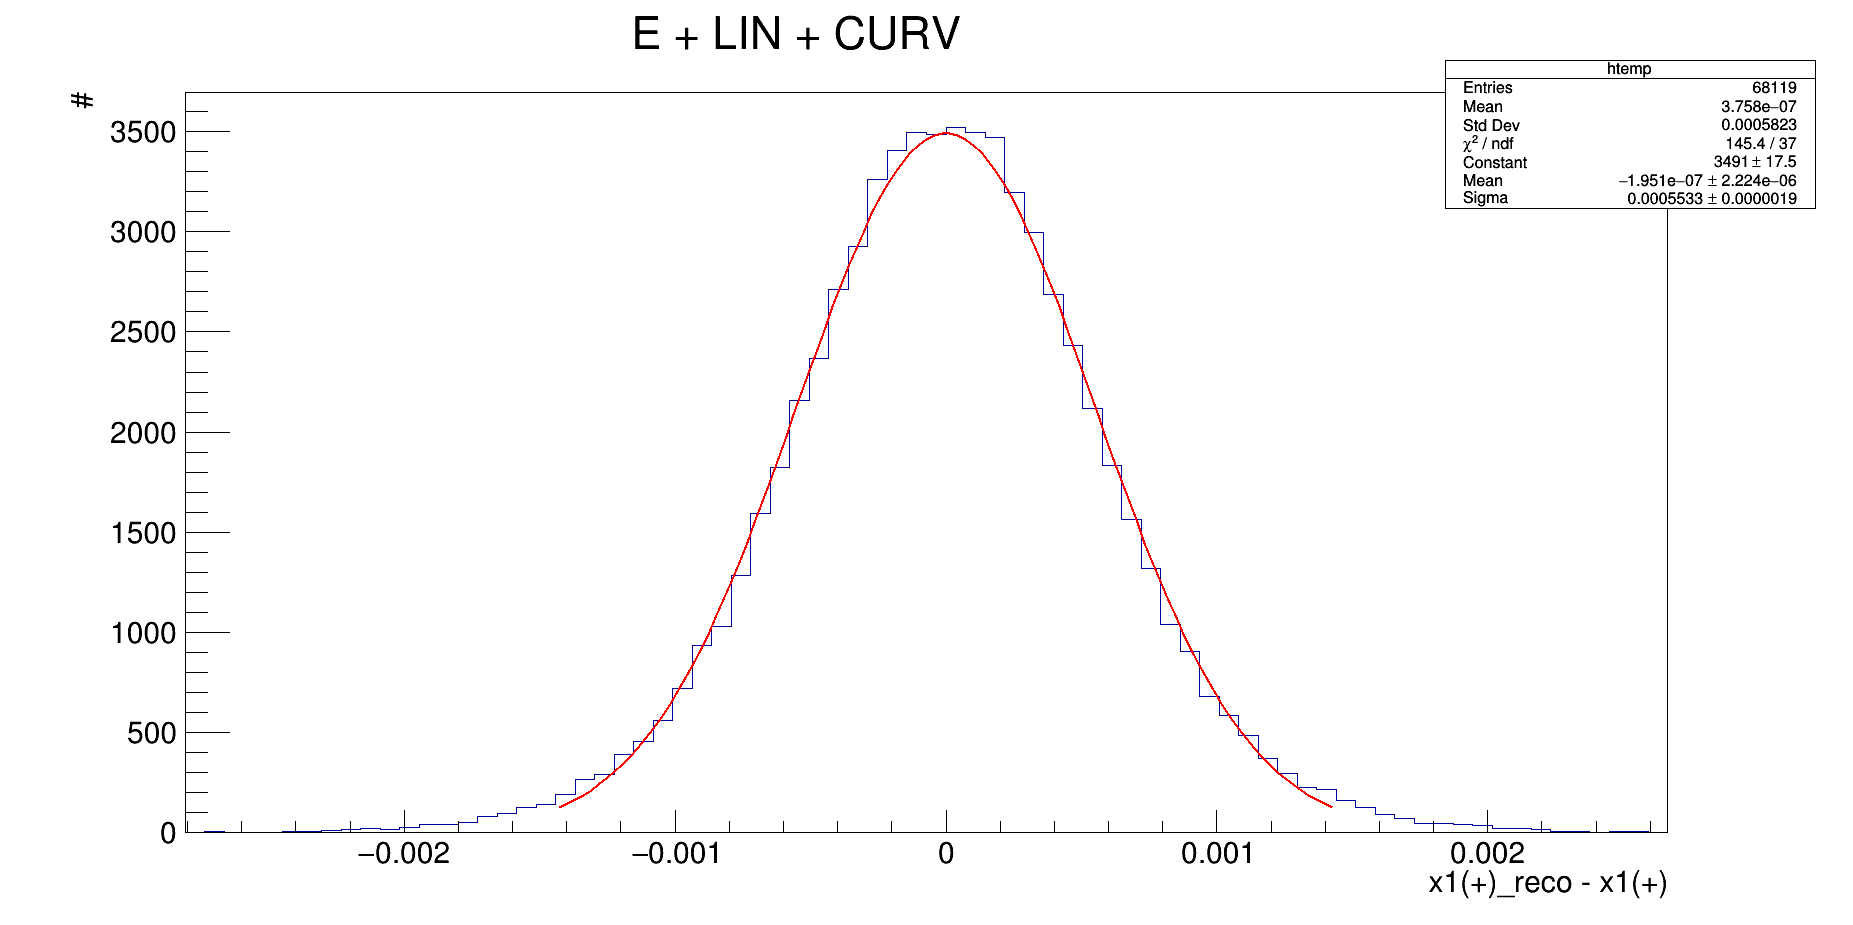
\includegraphics[scale=0.25]{set_2_x} 
		\caption{Risoluzione di $x_1^+$ con il set di vincoli numero 2. La risoluzione è migliorata rispetto a quella del rivelatore (0.001).}
		\label{fig:set_2_x}
	\end{center}
\end{figure}

\begin{figure}[h!]
	\begin{center}
		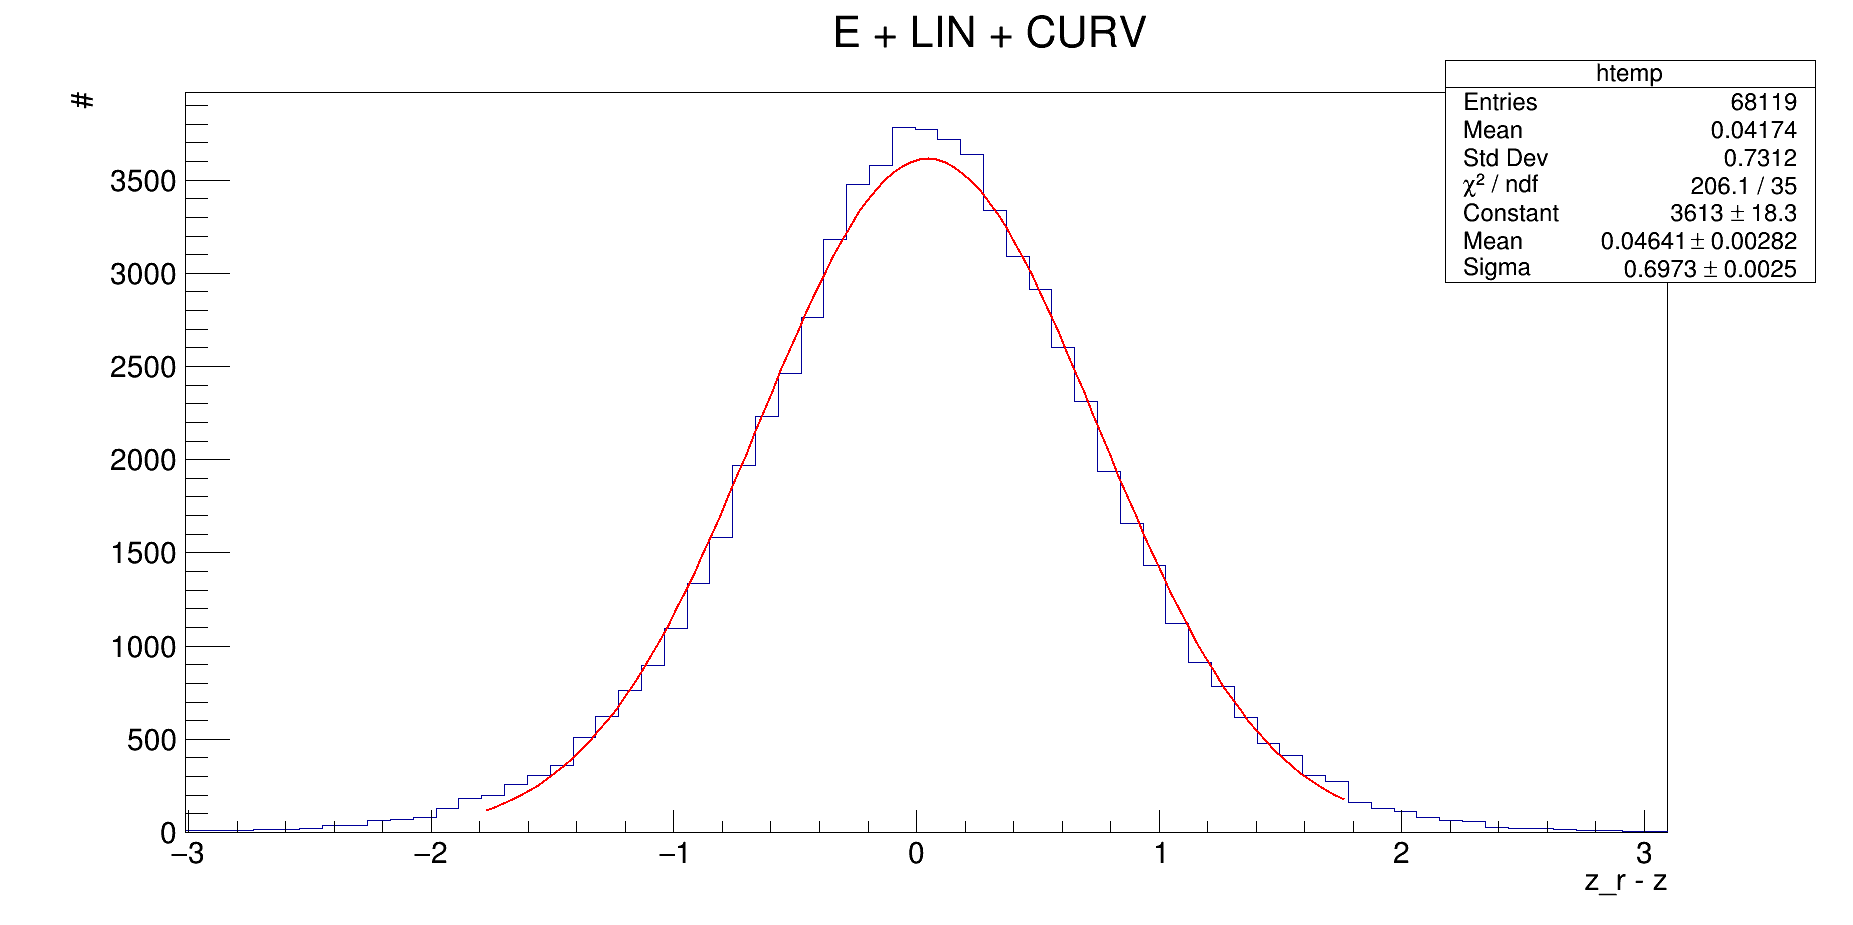
\includegraphics[scale=0.25]{set_2_z} 
		\caption{Risoluzione di $z_v$ con il set di vincoli numero 2.}
		\label{fig:set_2_z}
	\end{center}
\end{figure}

\begin{figure}[h!]
	\begin{center}
		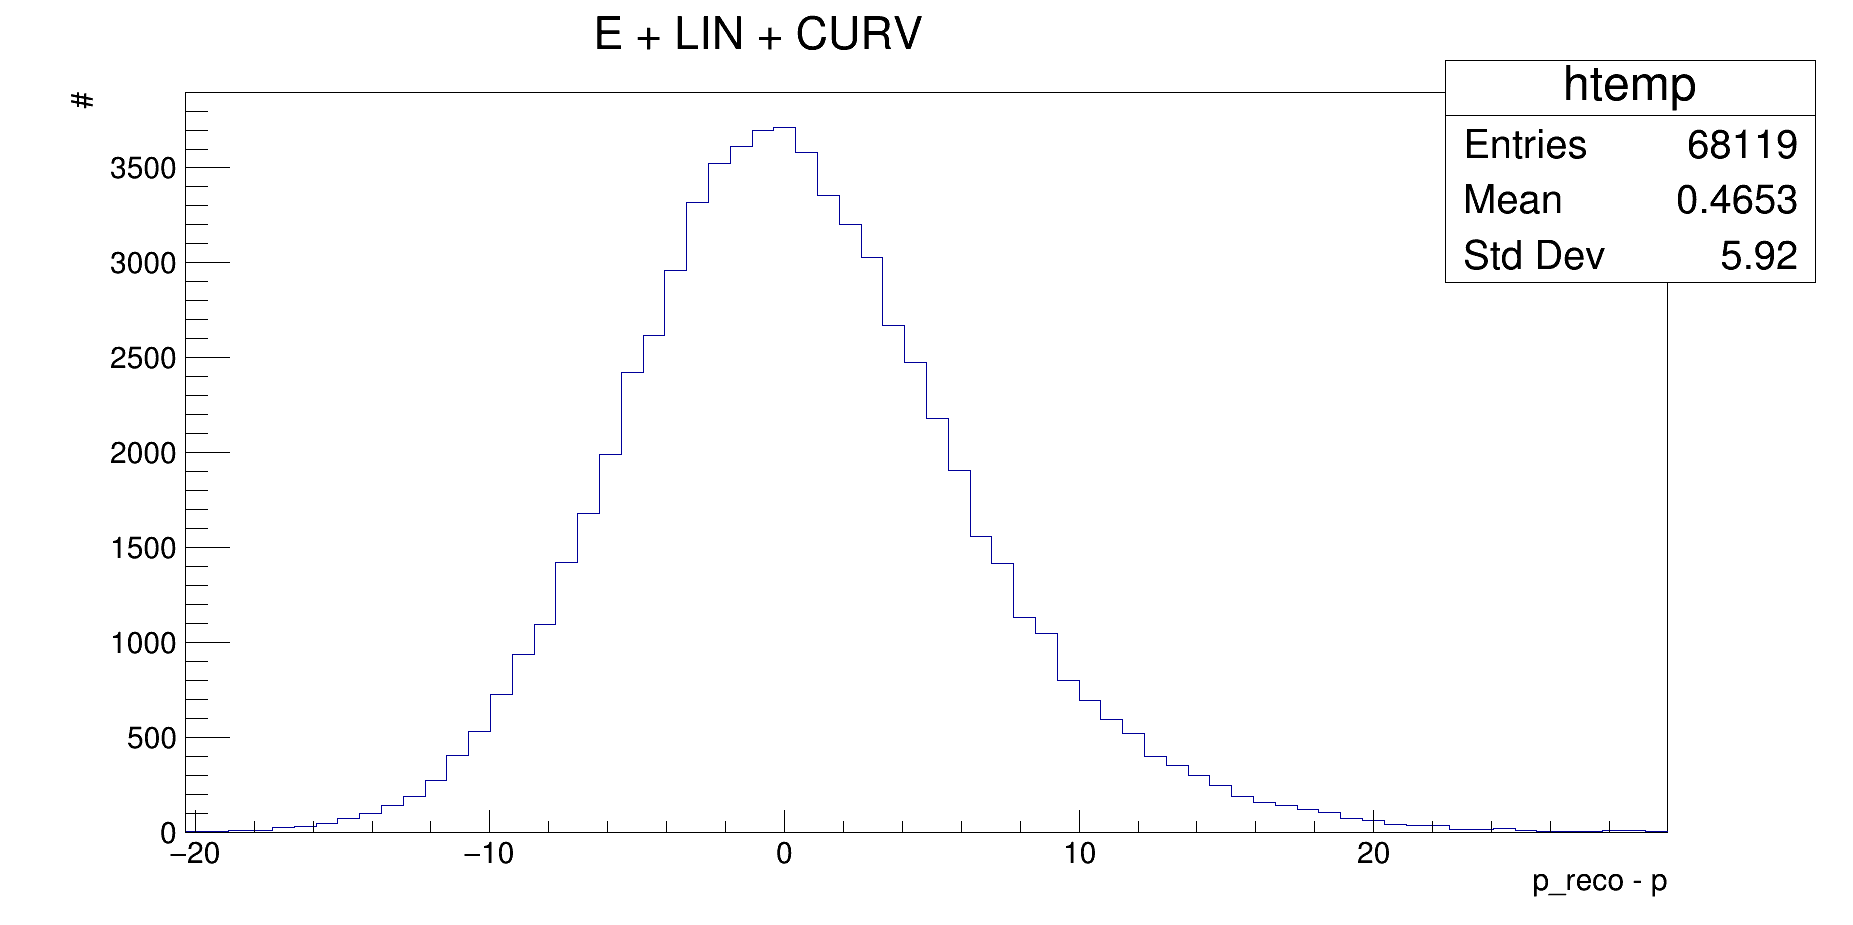
\includegraphics[scale=0.25]{set_2_p} 
		\caption{Risoluzione dell'impulso del $K^0$ con il set di vincoli numero 2. L'impulso è calcolato come $p^+ + p^-$, la parte angolare apporta un contributo trascurabile, a questa risoluzione.}
		\label{fig:set_2_p}
	\end{center}
\end{figure}

\begin{figure}[h!]
	\begin{center}
		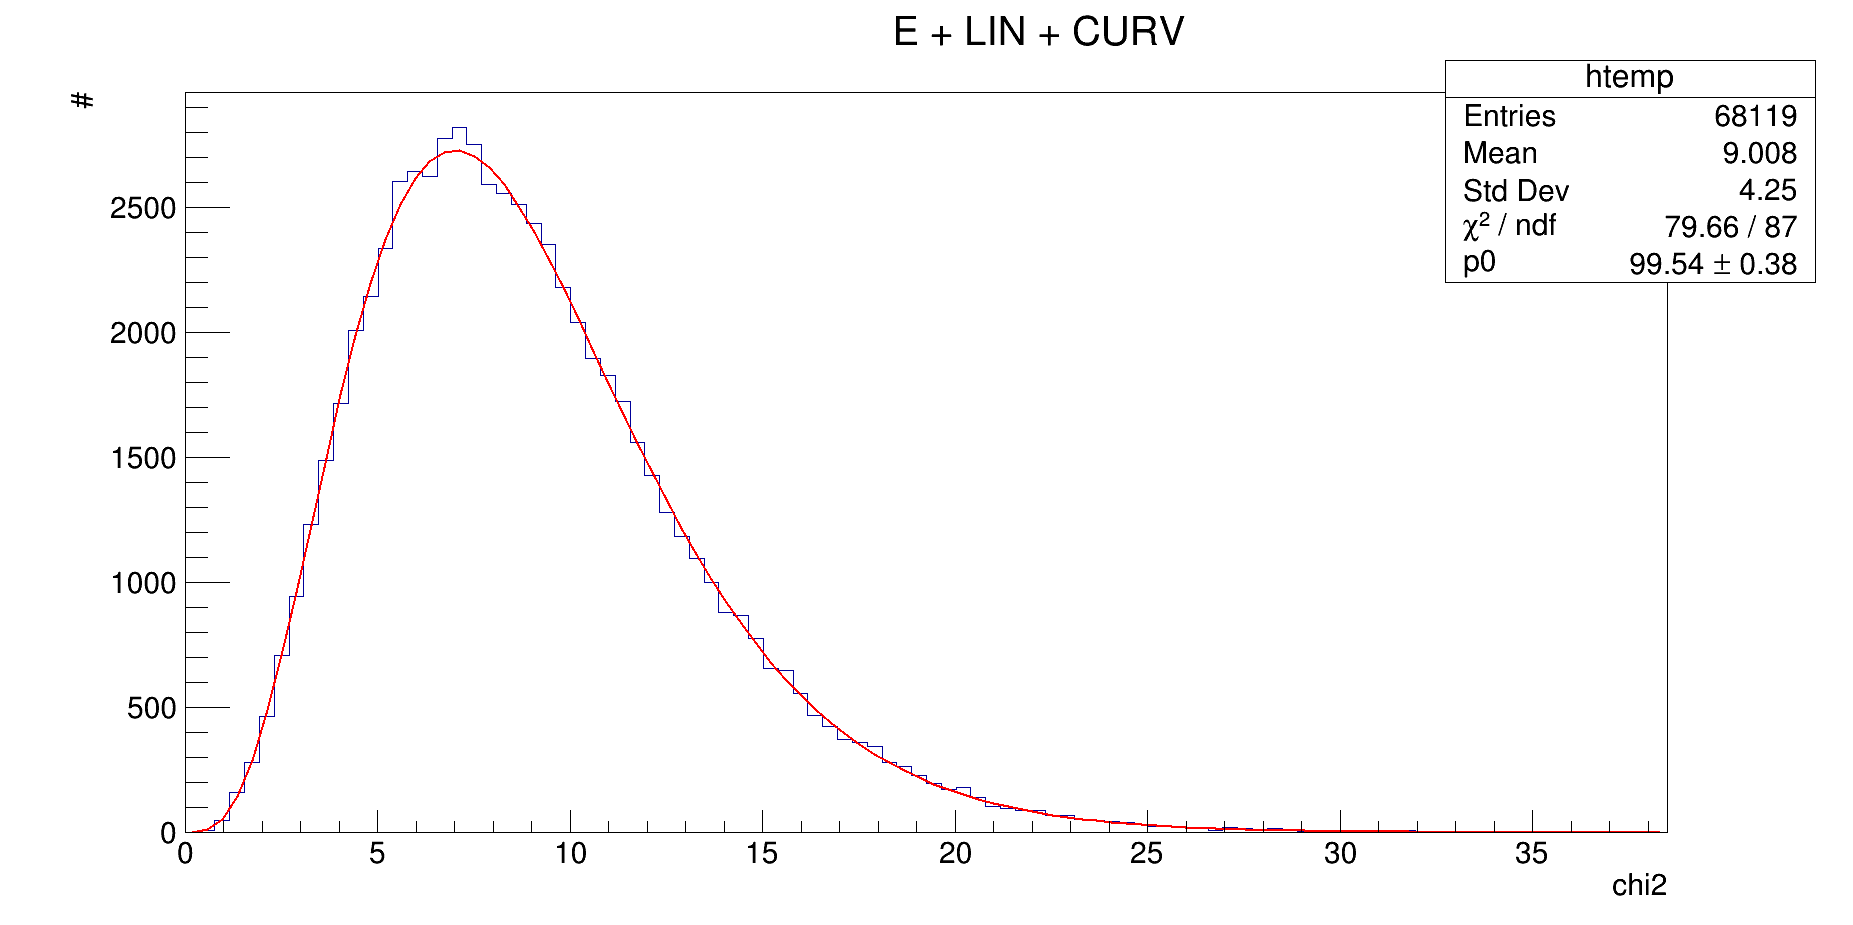
\includegraphics[scale=0.25]{set_2_chi2} 
		\caption{Distribuzione della funzione $X^2$ per il set di vincoli numero 2 e fit con una distribuzione $\chi^2_9$}
		\label{fig:set_2_chi2}
	\end{center}
\end{figure}

\begin{figure}[h!]
	\begin{center}
		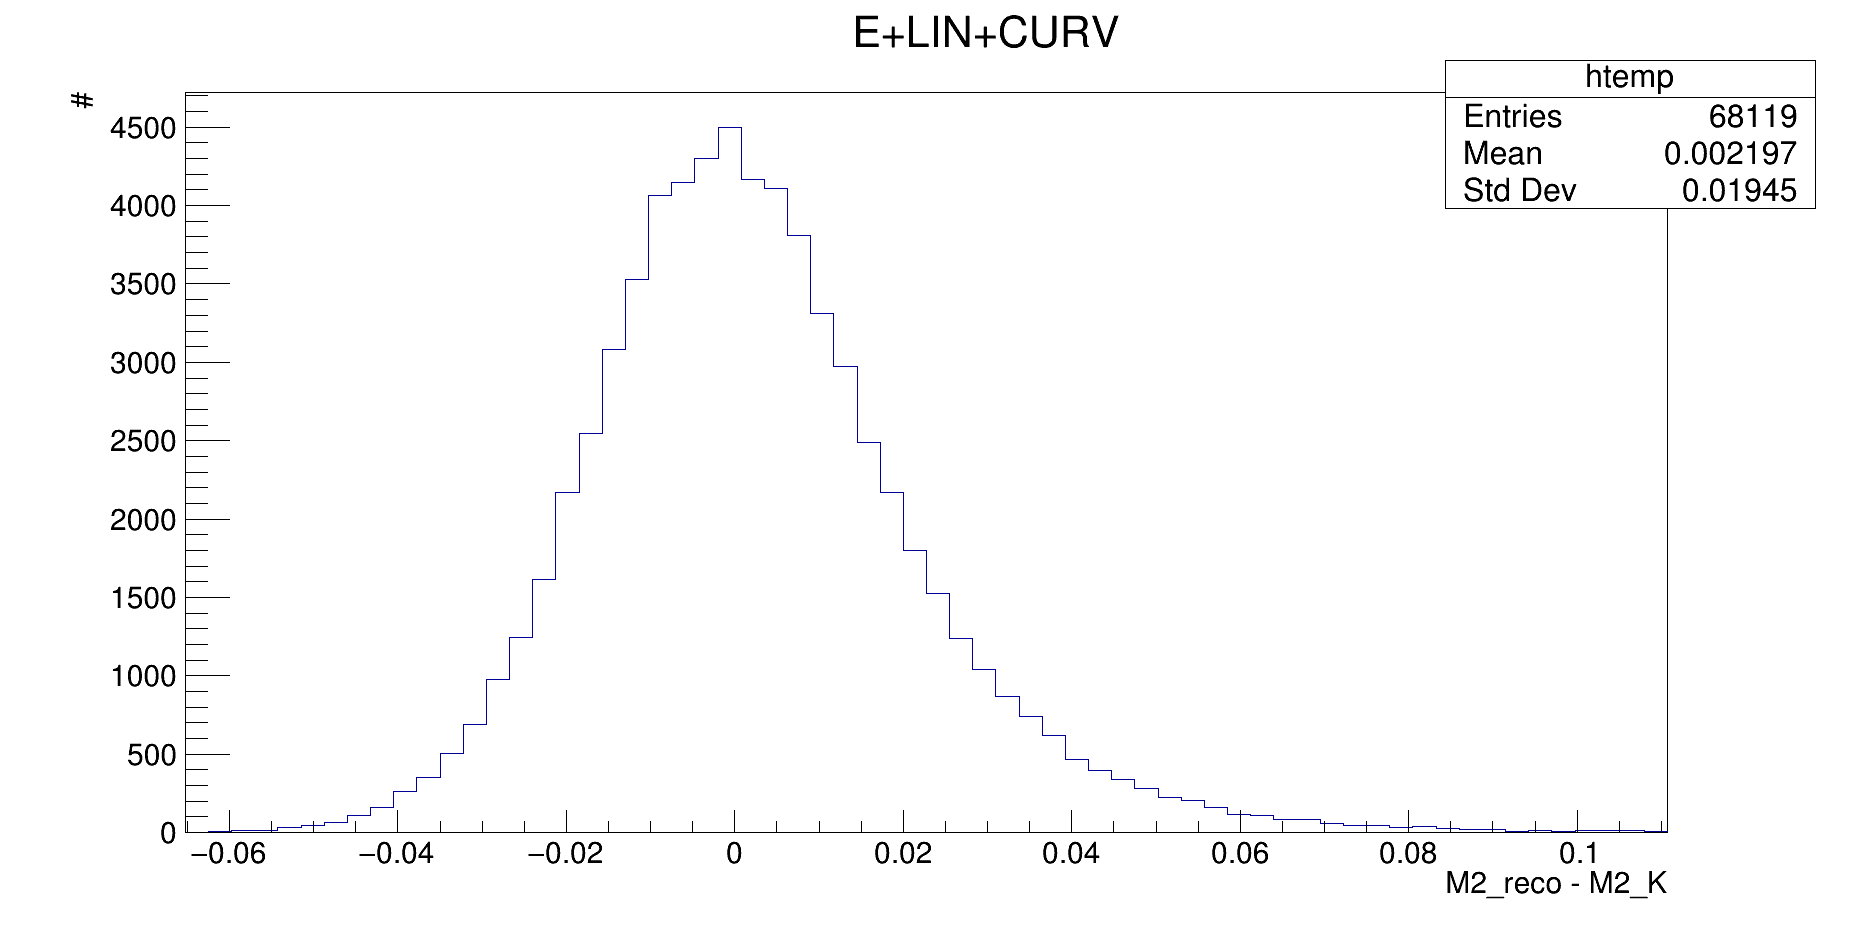
\includegraphics[scale=0.25]{set_2_inv} 
		\caption{Distribuzione della risoluzione di massa invariante per il set di vincoli numero 2.}
		\label{fig:set_2_inv}
	\end{center}
\end{figure}


\begin{figure}[h!]
	\begin{center}
		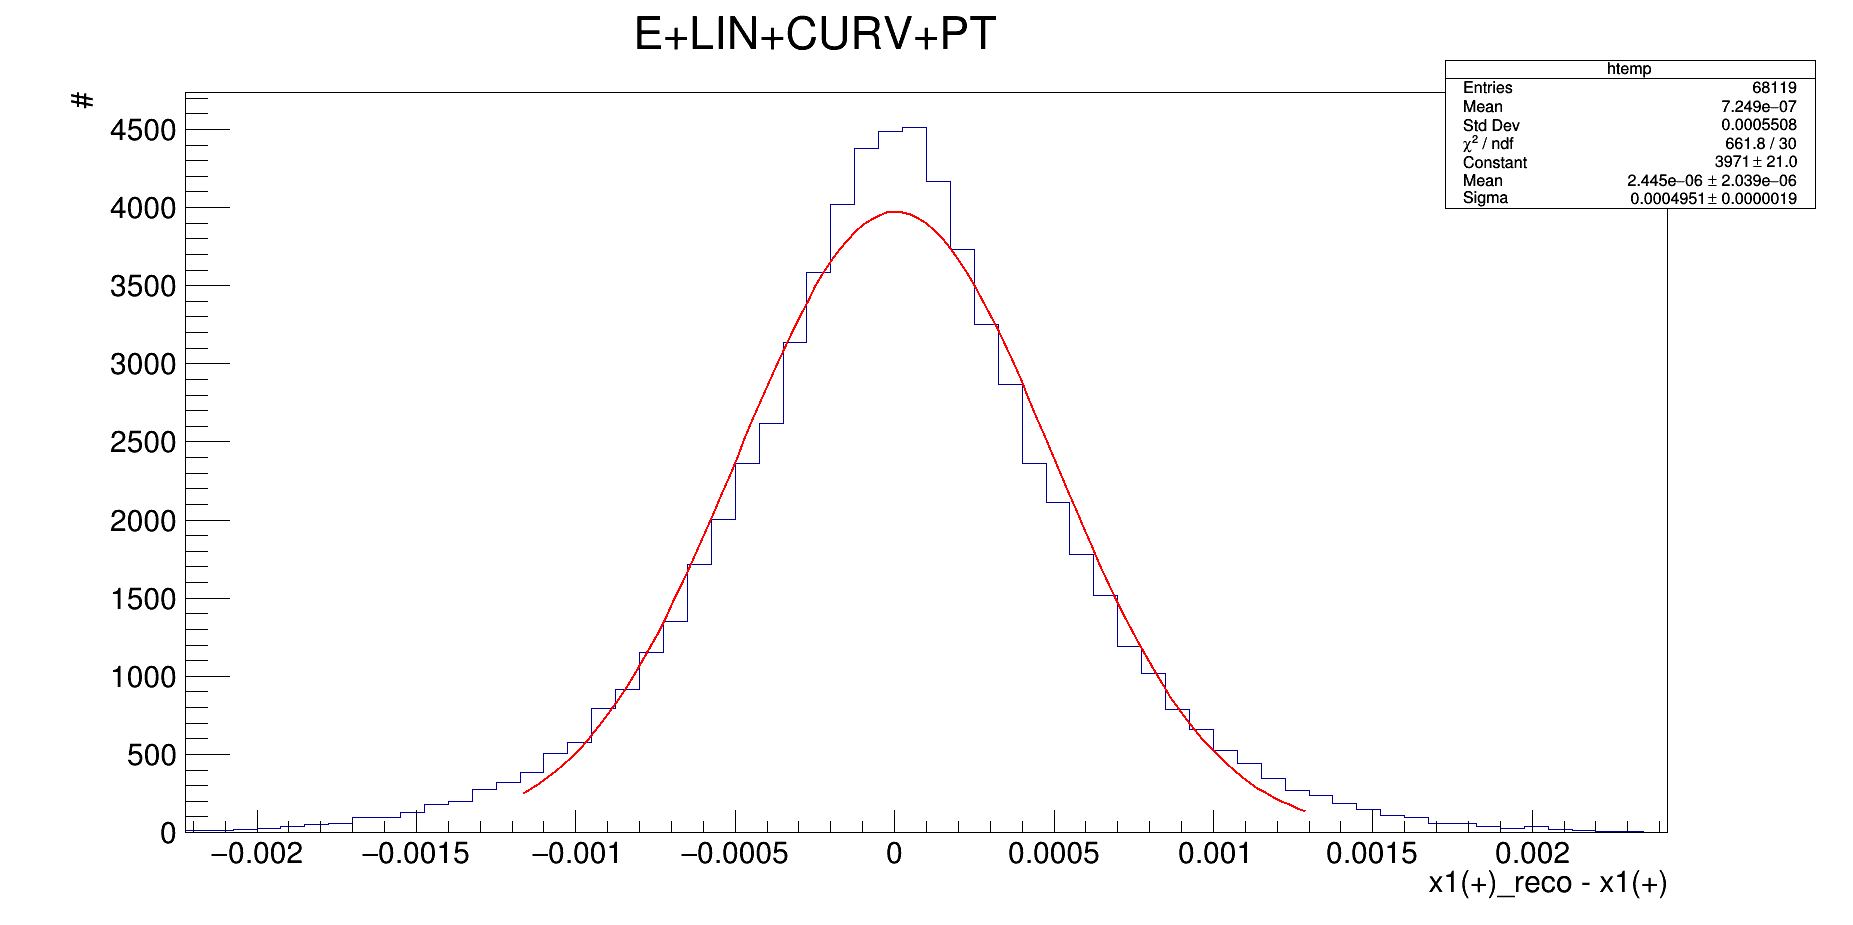
\includegraphics[scale=0.25]{set_3_x} 
		\caption{Risoluzione di $x_1^+$ con il set di vincoli numero 3. La risoluzione è migliorata rispetto a quella del rivelatore (0.001).}
		\label{fig:set_3_x}
	\end{center}
\end{figure}

\begin{figure}[h!]
	\begin{center}
		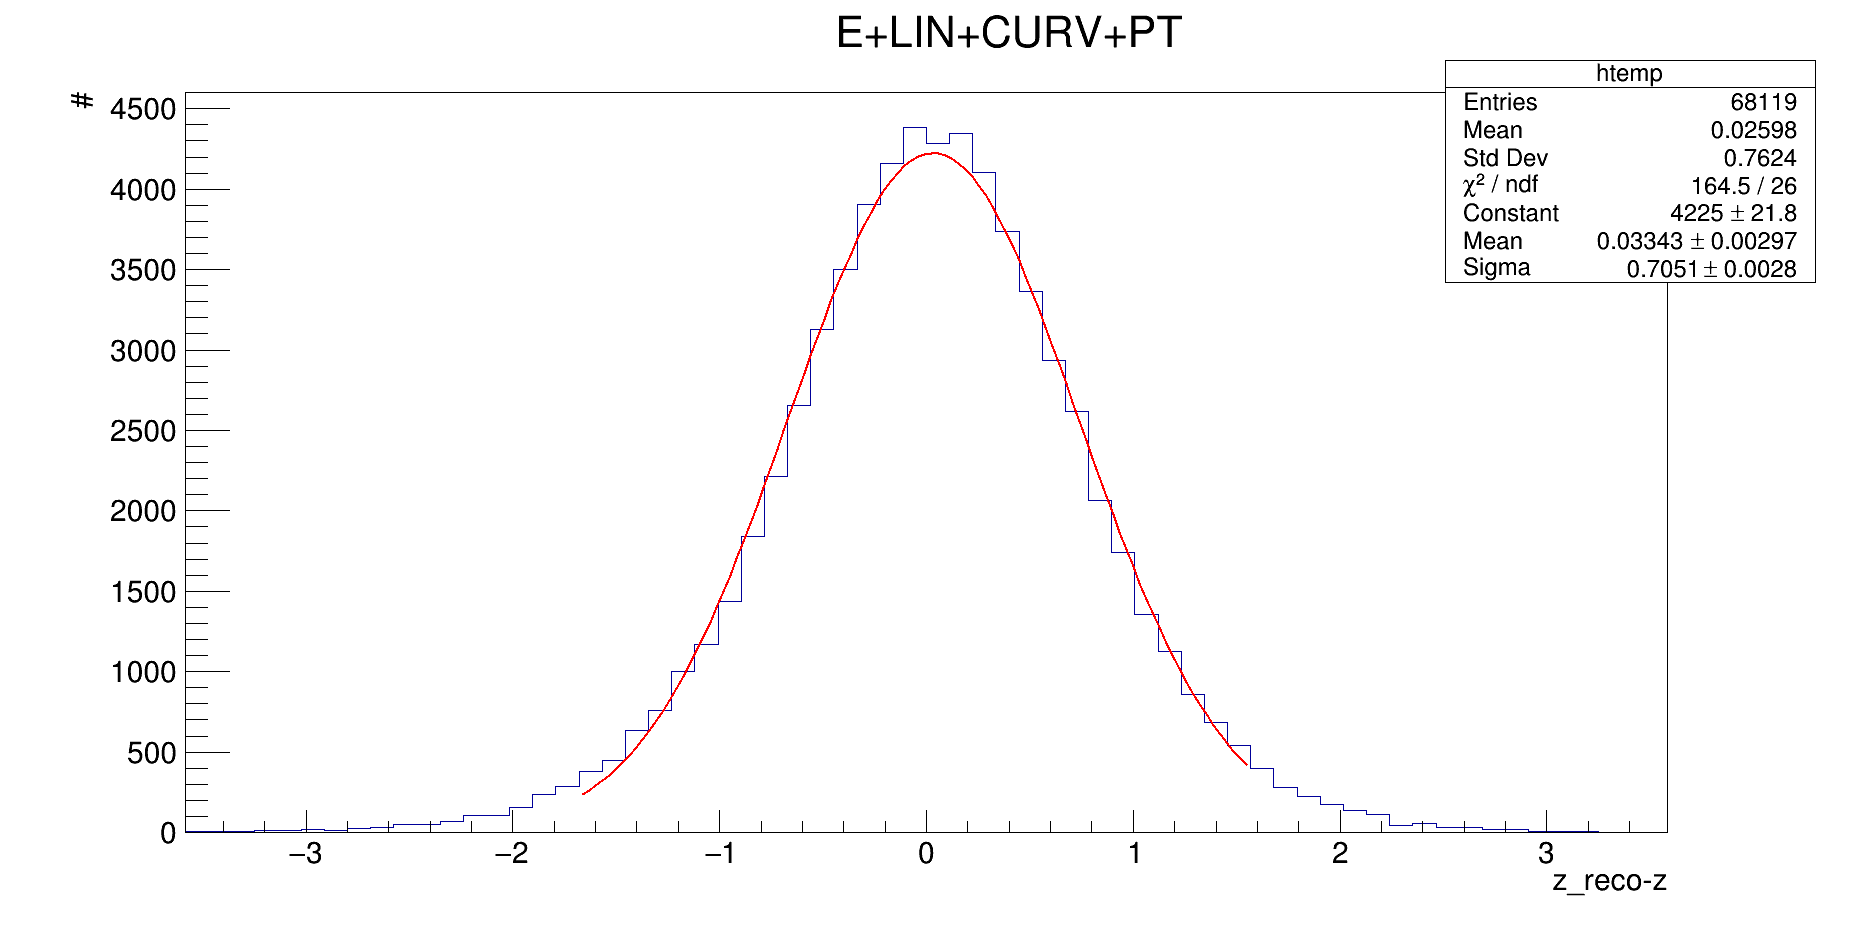
\includegraphics[scale=0.25]{set_3_z} 
		\caption{Risoluzione di $z_v$ con il set di vincoli numero 3.}
		\label{fig:set_3_z}
	\end{center}
\end{figure}

\begin{figure}[h!]
	\begin{center}
		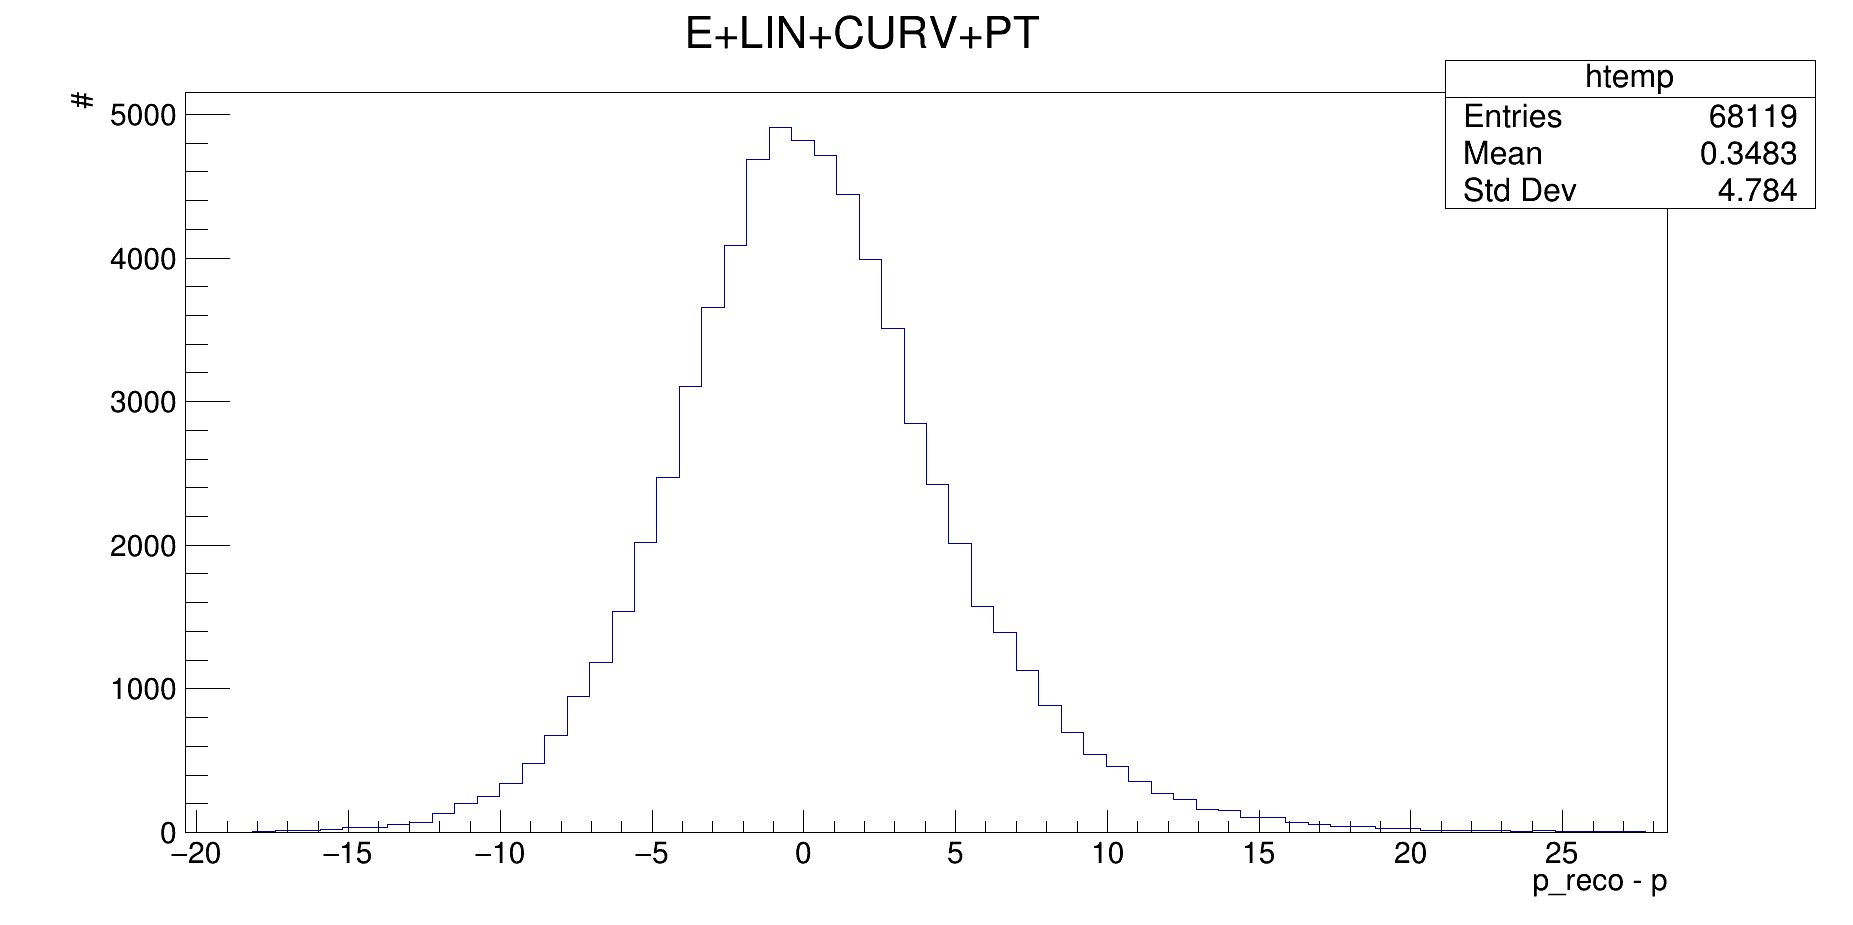
\includegraphics[scale=0.25]{set_3_p} 
		\caption{Risoluzione dell'impulso del $K^0$ con il set di vincoli numero 3. L'impulso è calcolato come $p^+ + p^-$, la parte angolare apporta un contributo trascurabile, a questa risoluzione.}
		\label{fig:set_3_p}
	\end{center}
\end{figure}

\begin{figure}[h!]
	\begin{center}
		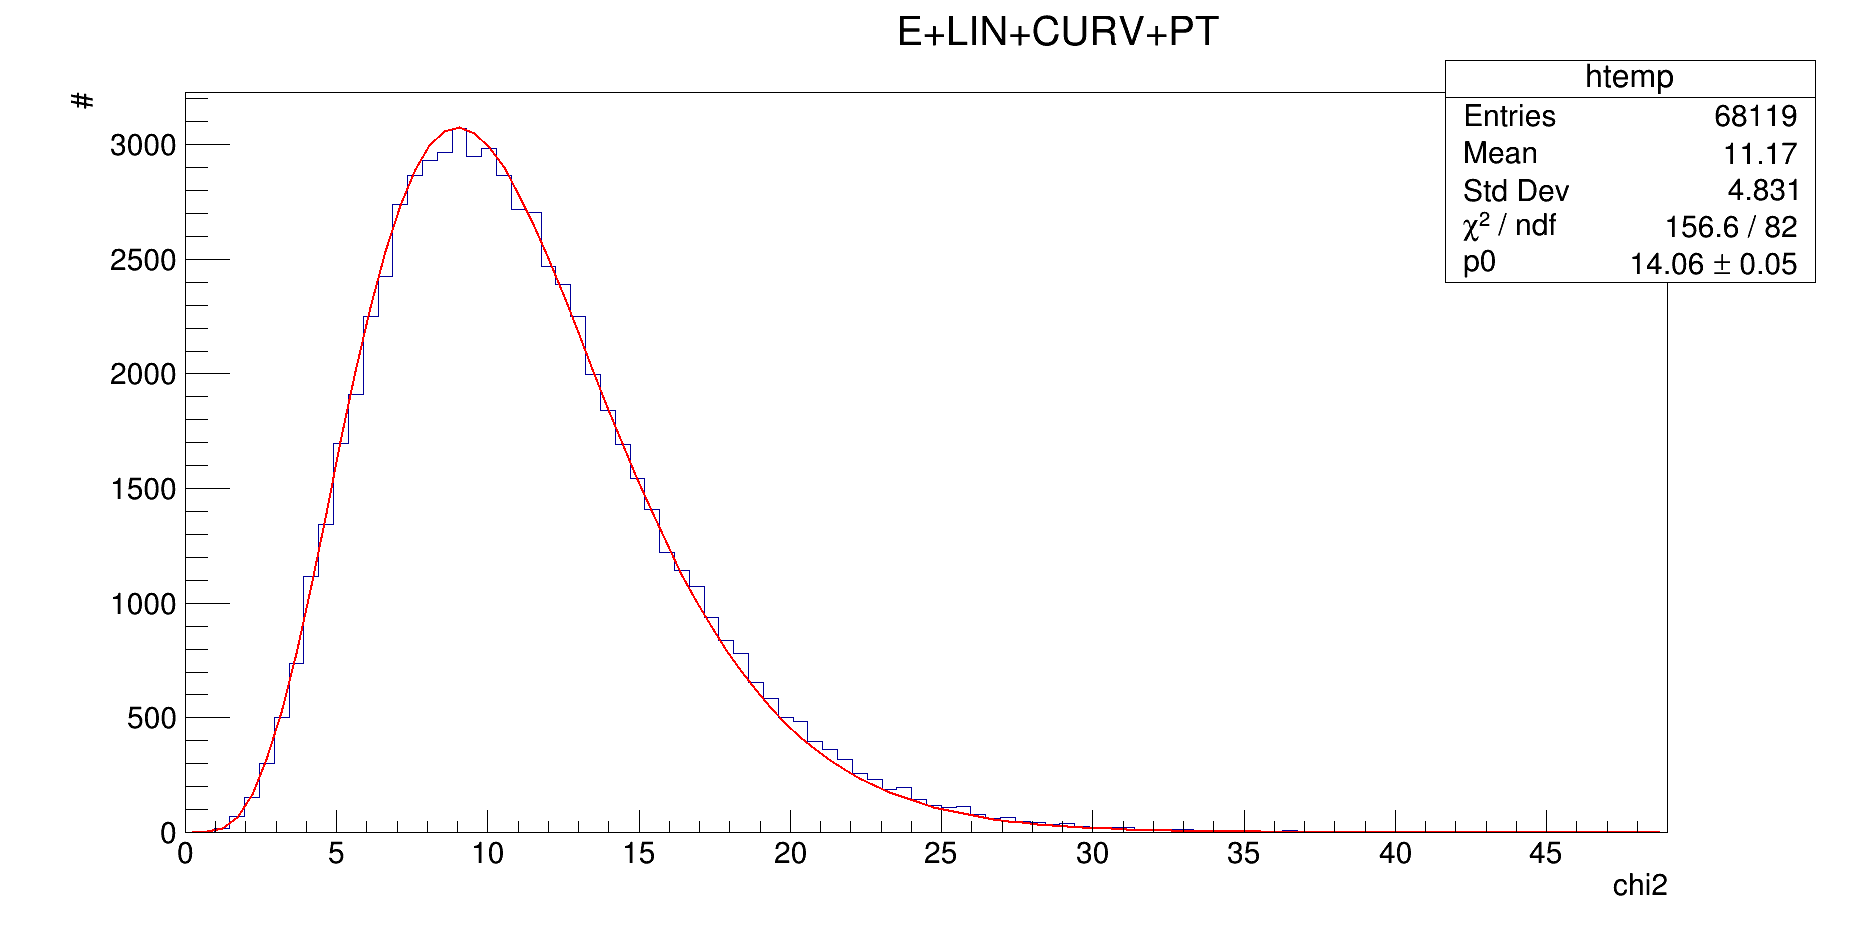
\includegraphics[scale=0.25]{set_3_chi2} 
		\caption{Distribuzione della funzione $X^2$ per il set di vincoli numero 3 e fit con una distribuzione $\chi^2_{11}$}
		\label{fig:set_3_chi2}
	\end{center}
\end{figure}

\begin{figure}[h!]
	\begin{center}
		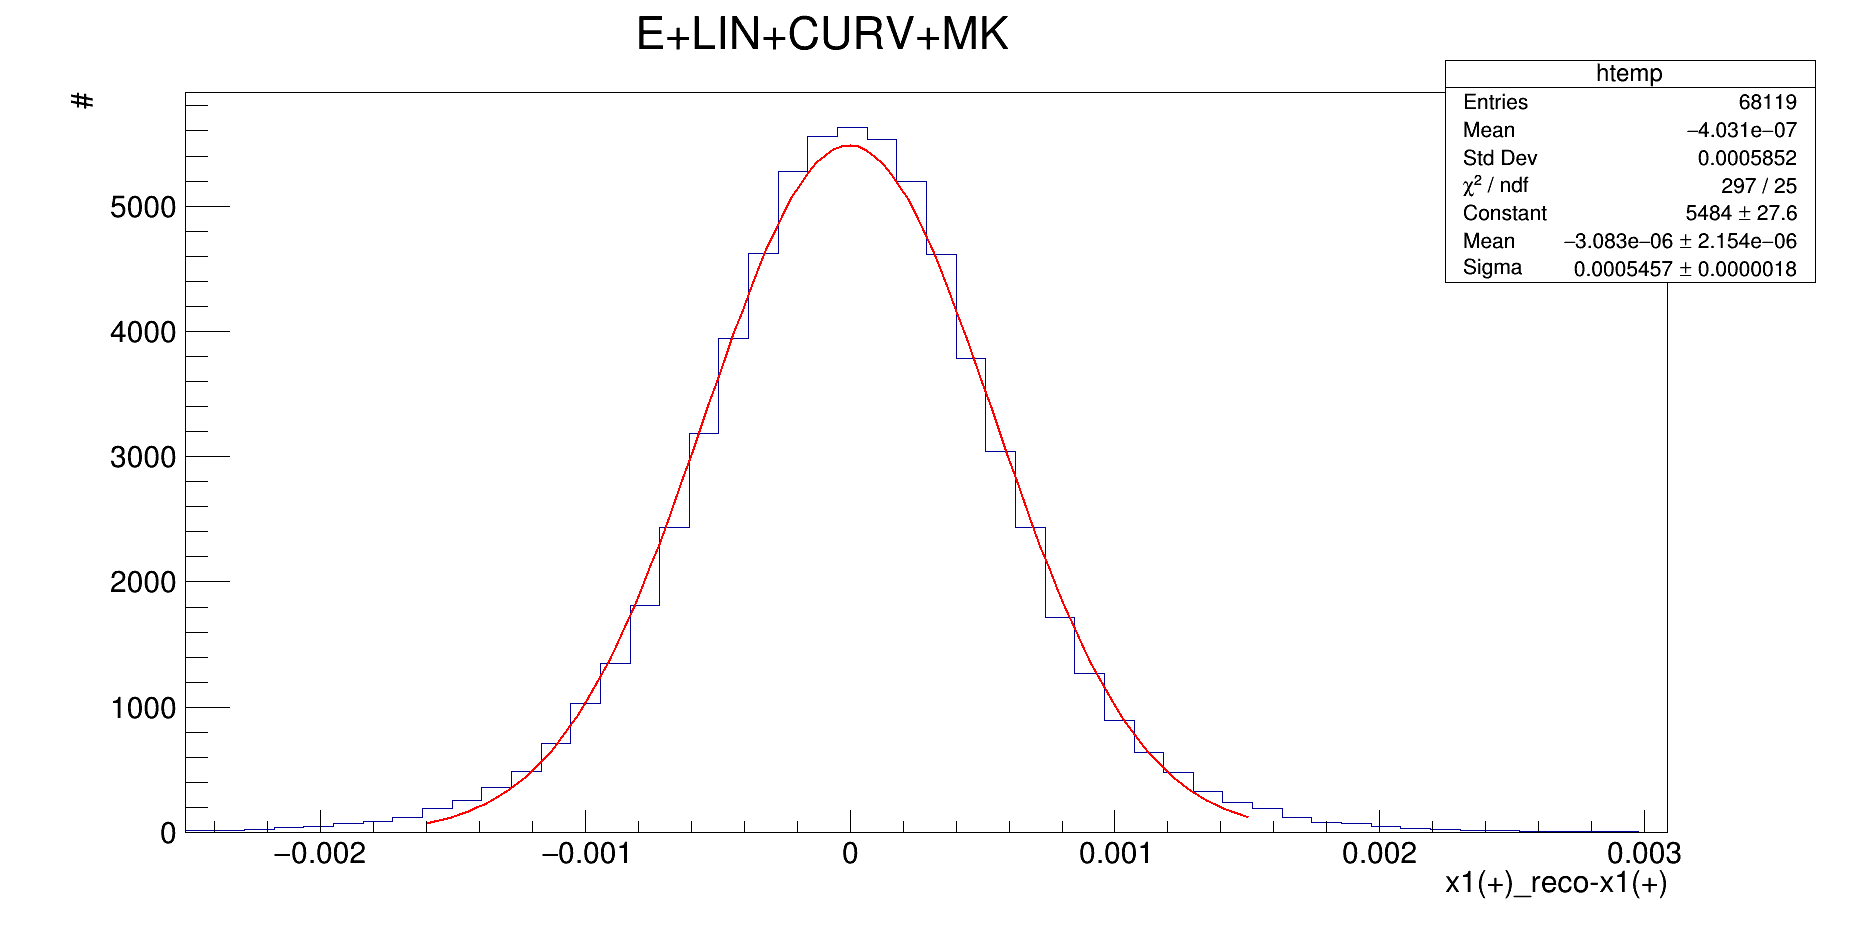
\includegraphics[scale=0.25]{set_4_x} 
		\caption{Risoluzione di $x_1^+$ con il set di vincoli numero 4. La risoluzione è migliorata rispetto a quella del rivelatore (0.001).}
		\label{fig:set_4_x}
	\end{center}
\end{figure}

\begin{figure}[h!]
	\begin{center}
		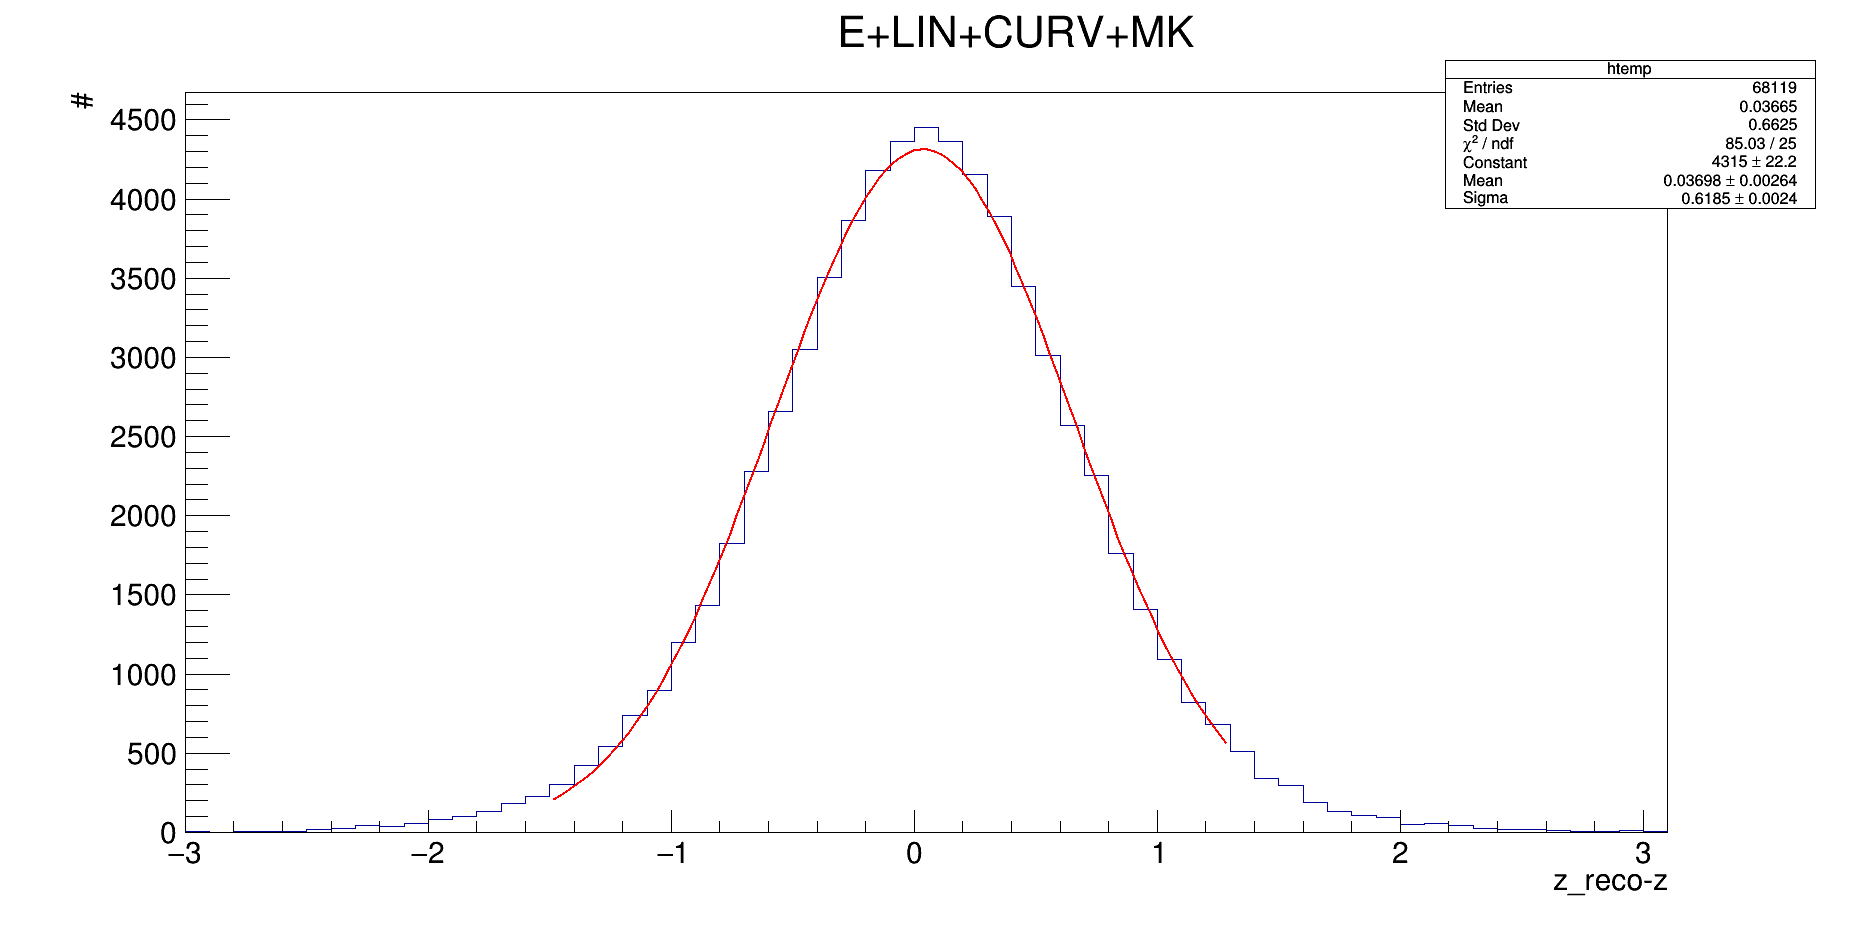
\includegraphics[scale=0.25]{set_4_z} 
		\caption{Risoluzione di $z_v$ con il set di vincoli numero 4.}
		\label{fig:set_4_z}
	\end{center}
\end{figure}

\begin{figure}[h!]
	\begin{center}
		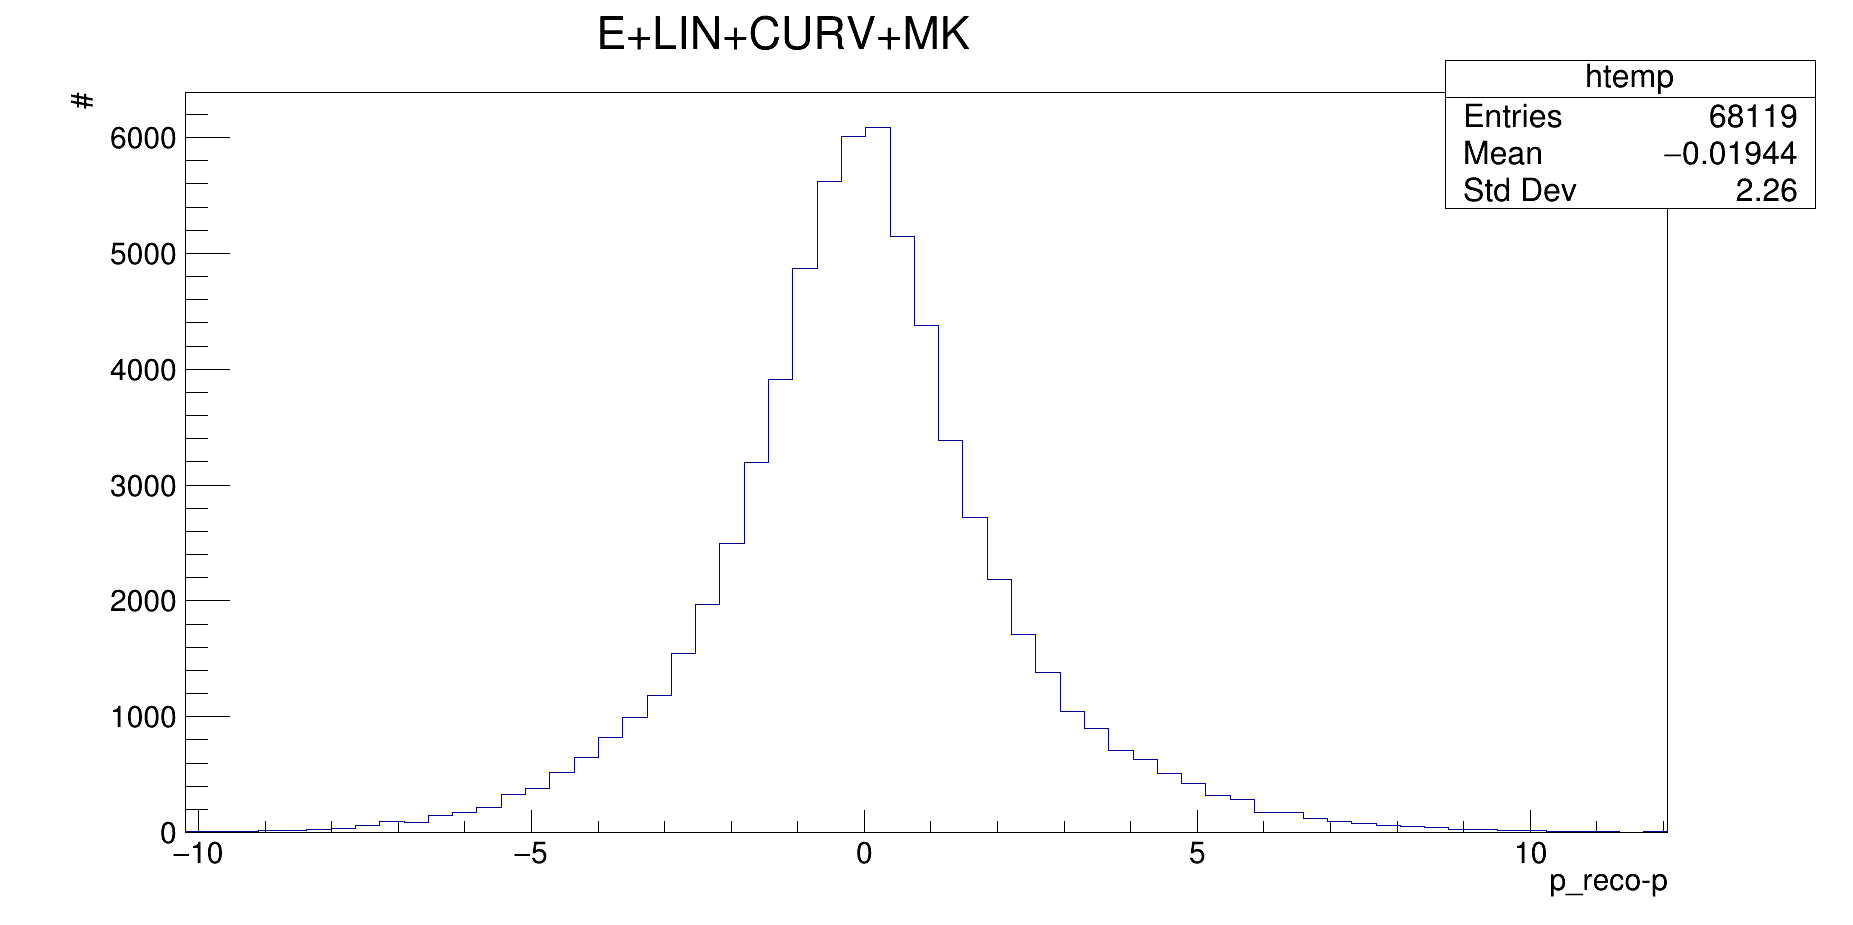
\includegraphics[scale=0.25]{set_4_p} 
		\caption{Risoluzione dell'impulso del $K^0$ con il set di vincoli numero 4. L'impulso è calcolato come $p^+ + p^-$, la parte angolare apporta un contributo trascurabile, a questa risoluzione.}
		\label{fig:set_4_p}
	\end{center}
\end{figure}

\begin{figure}[h!]
	\begin{center}
		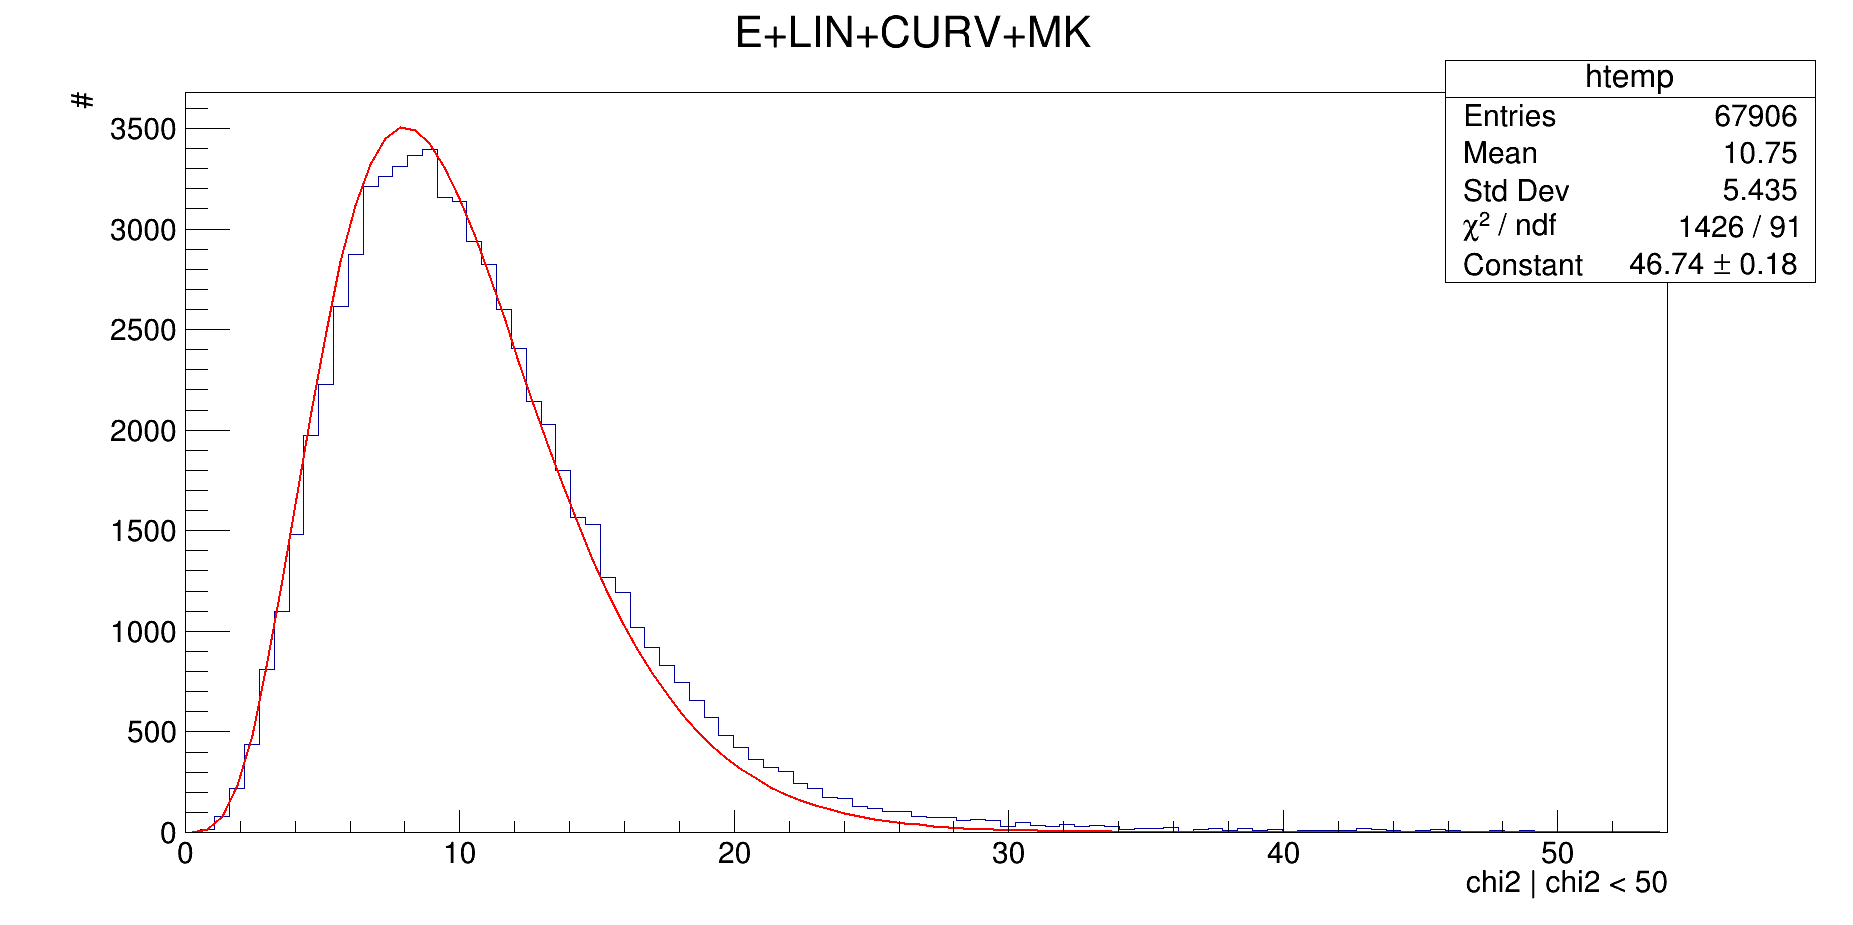
\includegraphics[scale=0.25]{set_4_chi2} 
		\caption{Distribuzione della funzione $X^2$ per il set di vincoli numero 4 e fit con una distribuzione $\chi^2_{10}$}
		\label{fig:set_4_chi2}
	\end{center}
\end{figure}

\begin{figure}[h!]
	\begin{center}
		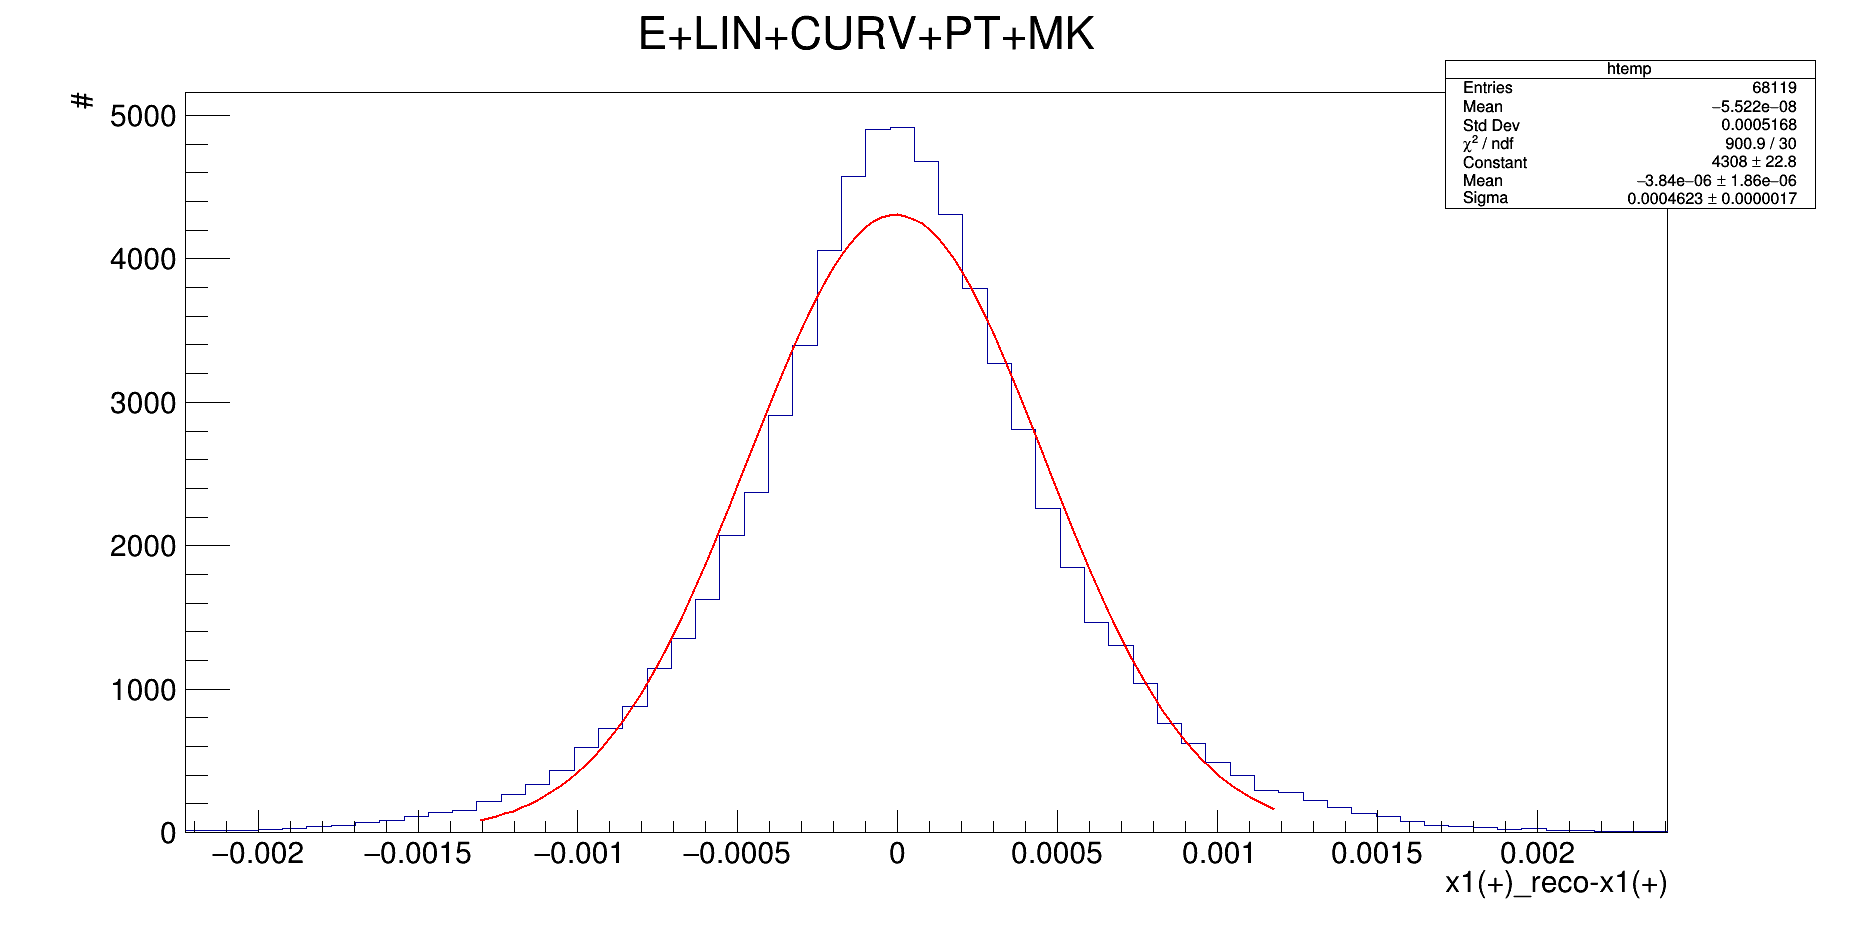
\includegraphics[scale=0.25]{set_5_x} 
		\caption{Risoluzione di $x_1^+$ con il set di vincoli numero 5. La risoluzione è migliorata rispetto a quella del rivelatore (0.001).}
		\label{fig:set_5_x}
	\end{center}
\end{figure}

\clearpage

\begin{figure}[h!]
	\begin{center}
		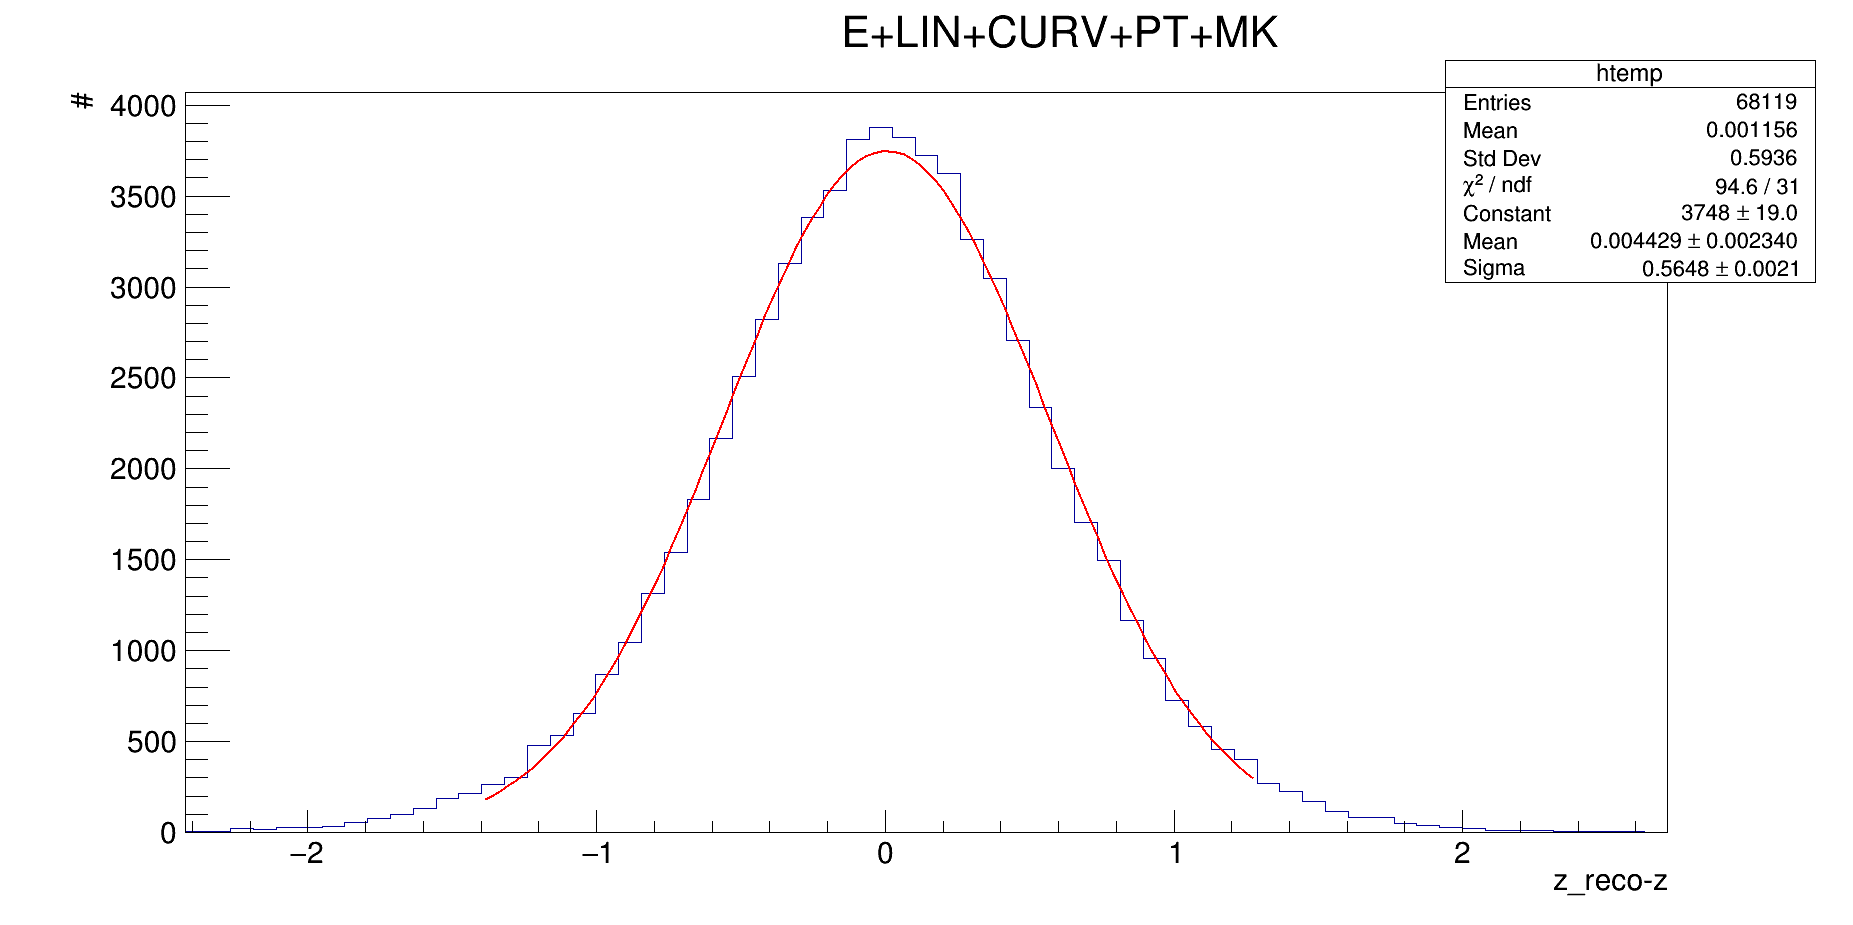
\includegraphics[scale=0.25]{set_5_z} 
		\caption{Risoluzione di $z_v$ con il set di vincoli numero 5.}
		\label{fig:set_5_z}
	\end{center}
\end{figure}

\begin{figure}[h!]
	\begin{center}
		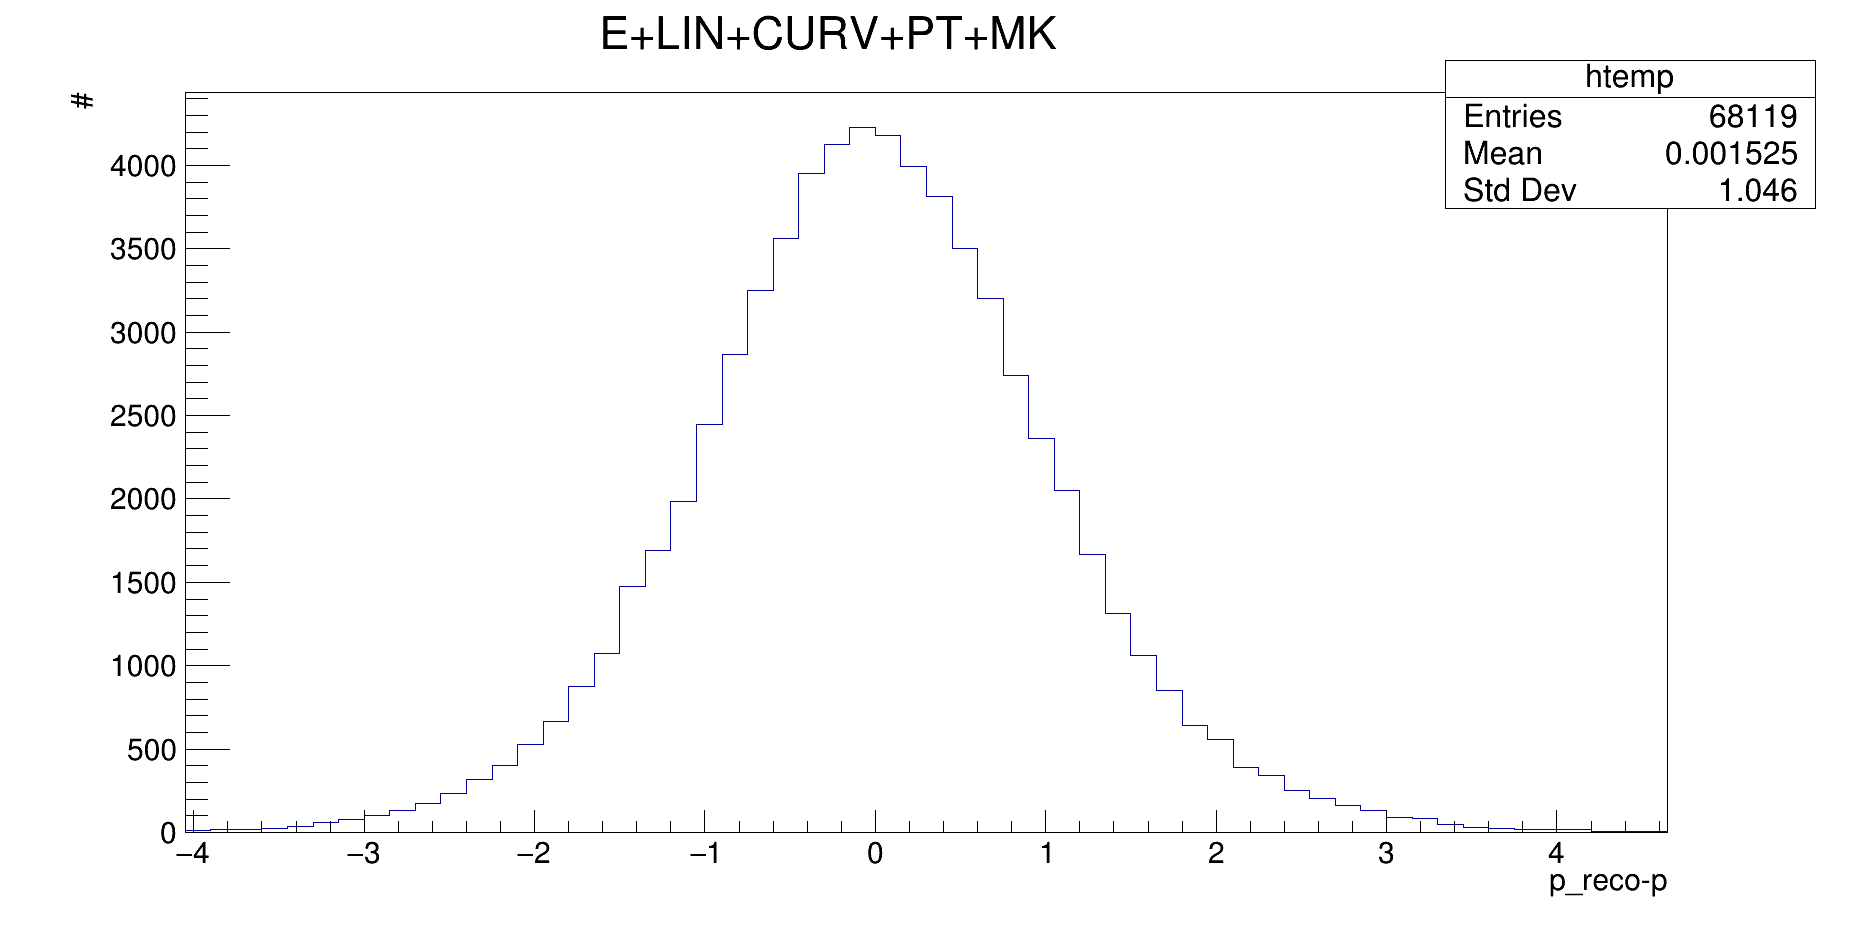
\includegraphics[scale=0.25]{set_5_p} 
		\caption{Risoluzione dell'impulso del $K^0$ con il set di vincoli numero 5. L'impulso è calcolato come $p^+ + p^-$, la parte angolare apporta un contributo trascurabile, a questa risoluzione.}
		\label{fig:set_5_p}
	\end{center}
\end{figure}

\begin{figure}[h!]
	\begin{center}
		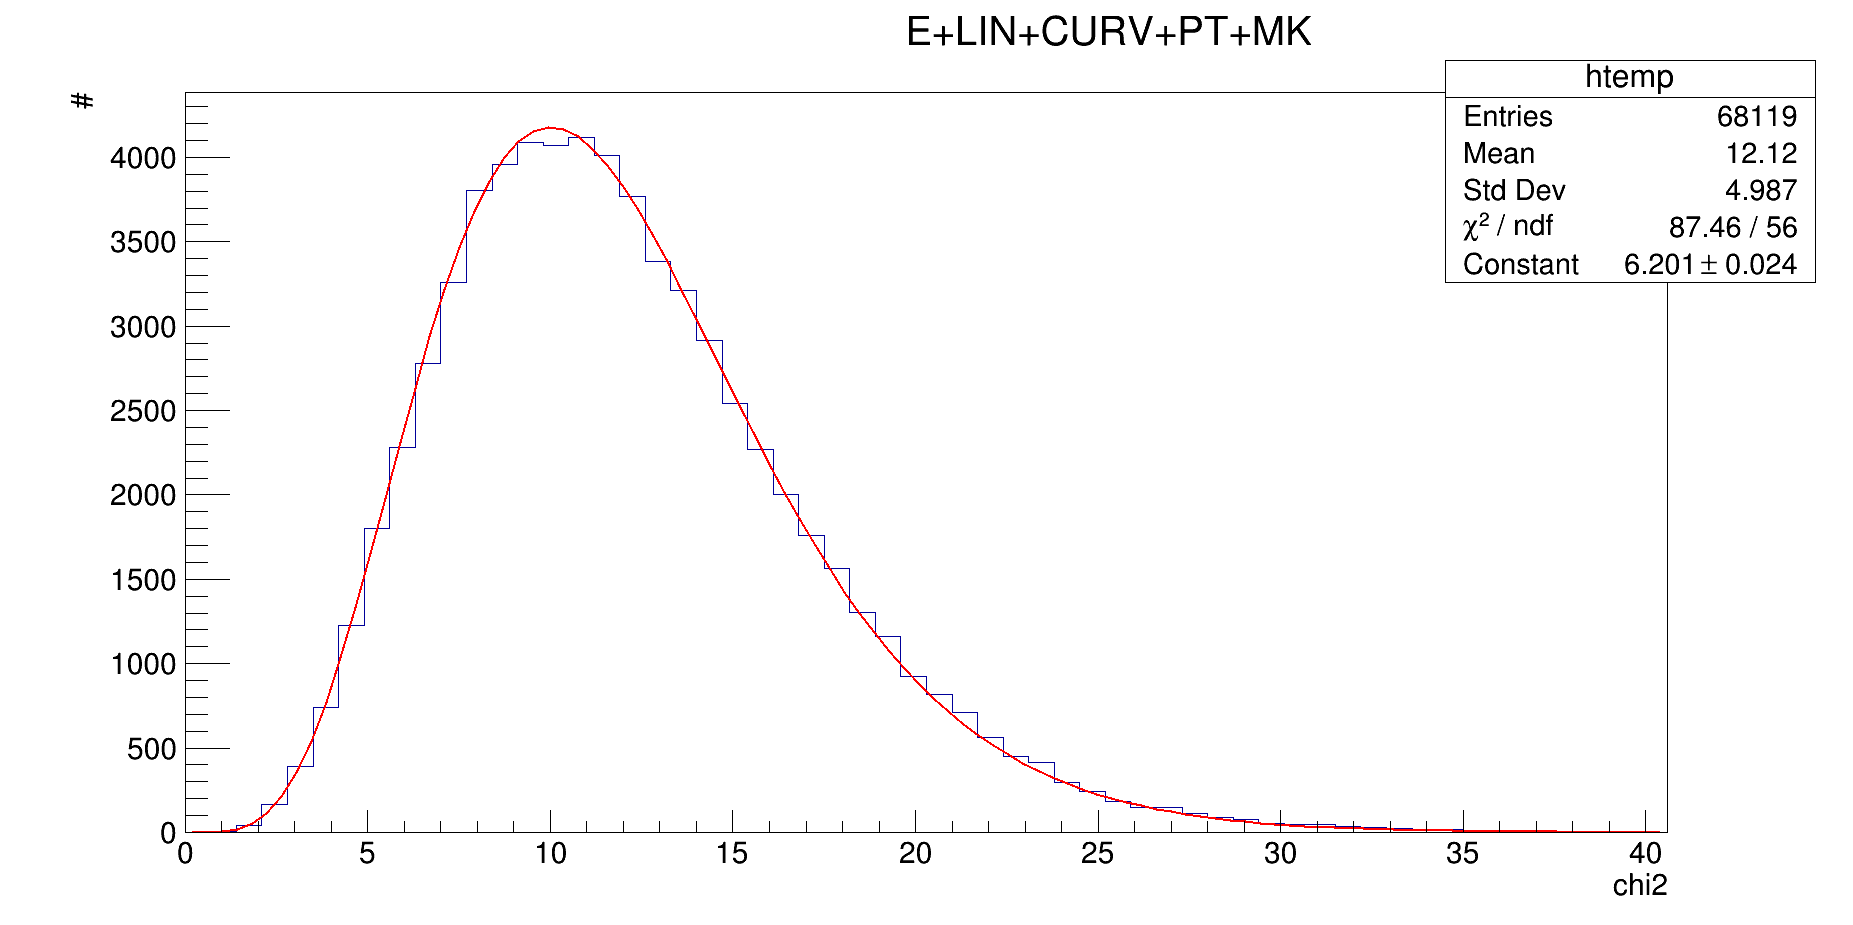
\includegraphics[scale=0.25]{set_5_chi2} 
		\caption{Distribuzione della funzione $X^2$ per il set di vincoli numero 5 e fit con una distribuzione $\chi^2_{12}$}
		\label{fig:set_5_chi2}
	\end{center}
\end{figure}

\begin{figure}[h!]
	\begin{center}
		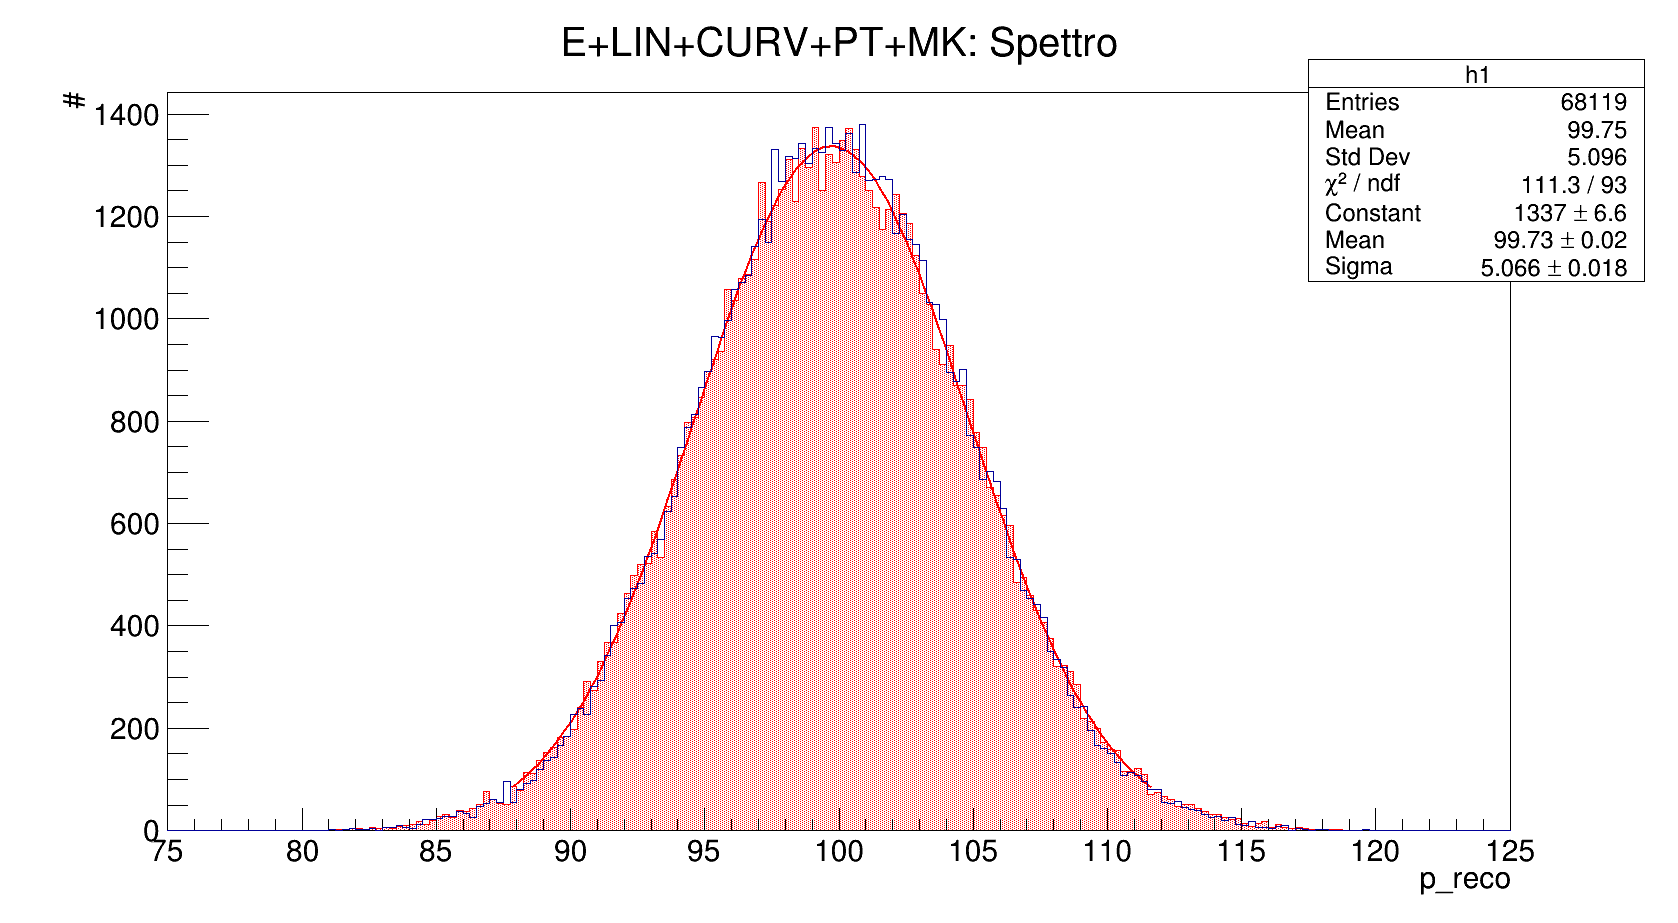
\includegraphics[scale=0.25]{set_5_spettro} 
		\caption{Ricostruzione dello spettro di impulso del $K^0$ per il set di vincoli numero 5. In rosso lo spettro ricostruito, in blu quello generato.}
		\label{fig:set_5_spettro}
	\end{center}
\end{figure}

\begin{figure}[h!]
	\begin{center}
		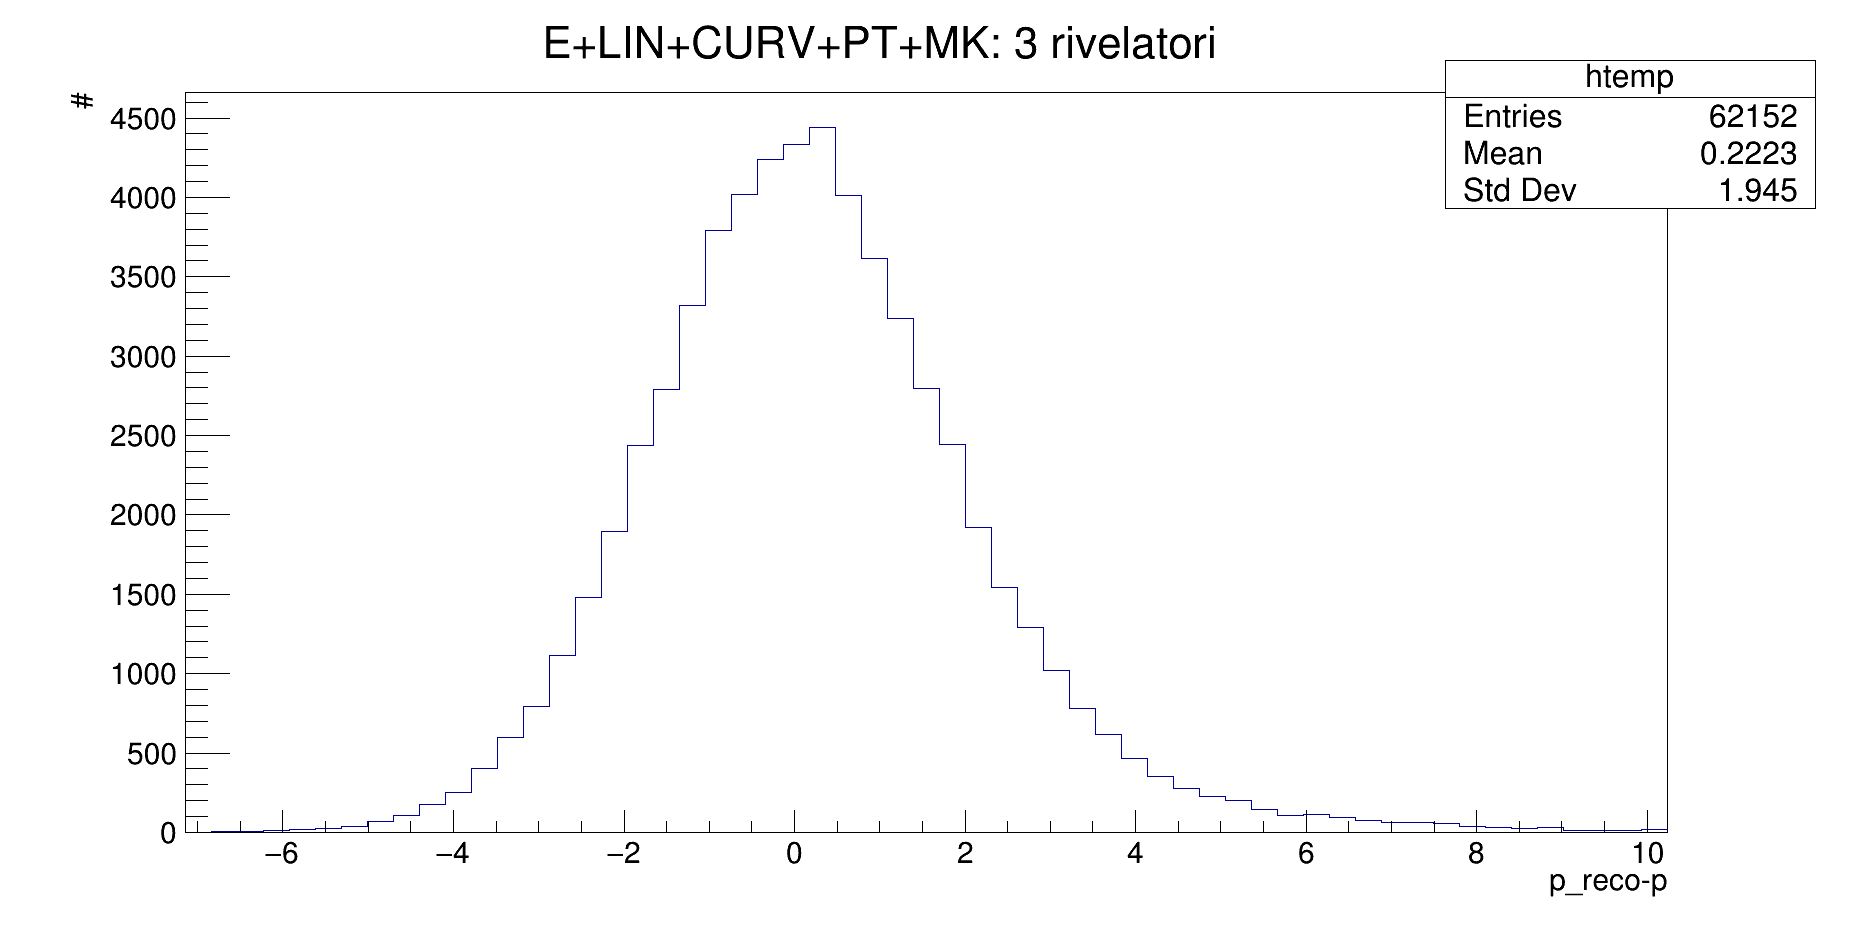
\includegraphics[scale=0.25]{set_1det_p} 
		\caption{Risoluzione della determinazione dell'impulso del $K^0$ usando tre rivelatori e un fit E + LIN + CURV + PT + MK.}
		\label{fig:set_1det_p}
	\end{center}
\end{figure}

\clearpage


\subsection{Valori numerici utilizzati e unità di misura}
\begin{itemize}
\item $c = 299792458\ m/s$
\item $M_K = 497.614\ MeV/c^2$
\item $M_\pi = 139.57018\ MeV/c^2$
\item $\tau = 8.954\cdot 10^{-11}\ s$
\end{itemize}

Le unità di misura, laddove non indicate, sono da intendersi \textit{m} per le lunghezze, \textit{GeV} per le energie, \textit{GeV/c} per gli impulsi, \textit{$GeV/c^2$} per le masse, \textit{s} per i tempi.

\end{document}